%\documentclass[a4paper,12pt]{book}

\documentclass[a4paper,11pt]{book}

\usepackage[dutch]{babel}
\usepackage{graphicx}
\usepackage{url}
\usepackage[utf8]{inputenc}
\usepackage[T1]{fontenc}
\usepackage{listings}
\usepackage{courier}
\usepackage{color}
\usepackage{xcolor}
%\usepackage{url}
\usepackage{float}
\usepackage{caption}
\usepackage{subcaption}
\usepackage{hyperref} % verwijder dit package als TOC, referenties, footnotes, e.d. niet meer 'clickable' moeten zijn
\usepackage{makeidx}
\usepackage[nottoc]{tocbibind}

\usepackage{amsmath}
\usepackage{tikz}
\usepackage{epigraph}
\usepackage{lipsum}
\usepackage{csquotes}
%
% Zorgt voor headers die over de marge lopen
%
\usepackage{fancyhdr}
\pagestyle{fancy}
\addtolength{\headwidth}{\marginparsep}
\addtolength{\headwidth}{\marginparwidth}
\renewcommand{\chaptermark}[1]{\markboth{#1}{}}
\renewcommand{\sectionmark}[1]{\markright{\thesection\ #1}}
\fancyhf{}
\fancyhead[LE,RO]{\bfseries\thepage}
\fancyhead[LO]{\bfseries\rightmark}
\fancyhead[RE]{\bfseries\leftmark}
\fancypagestyle{plain}{%
\fancyhead{} % get rid of headers
\renewcommand{\headrulewidth}{0pt} % and the line
}

\renewcommand\epigraphflush{flushright}
\renewcommand\epigraphsize{\normalsize}
\setlength\epigraphwidth{0.7\textwidth}

\definecolor{titlepagecolor}{cmyk}{1,.60,0,.40}

\DeclareFixedFont{\titlefont}{T1}{ppl}{b}{it}{0.5in}

% Clear Header Style on the Last Empty Odd pages
\makeatletter
\def\cleardoublepage{\clearpage\if@twoside \ifodd\c@page\else%
    \hbox{}%
    \thispagestyle{empty}%              % Empty header styles
    \newpage%
    \if@twocolumn\hbox{}\newpage\fi\fi\fi}
%\def\printauthor{{\large \@author}}
\makeatother
\author{%
    Gerben Dierick \\
    \vspace{20pt} \\
    Pieter Philippaerts \\
    \vspace{20pt} \\
    Vander Straeten
    }

%
% Zorgt voor default sans serif font
%
\renewcommand{\familydefault}{\sfdefault}

\newcommand{\byte}[1]{\fcolorbox{black}{lightgray}{\texttt{{#1}}}}

\newcommand{\TODO}[1]{\textbf{\textcolor{red}{TODO:~#1}}}

%
% Zorgt voor sans font in math
%
\usepackage{sfmath}

\newcommand\titlepagedecoration{%
\begin{tikzpicture}[remember picture,overlay,shorten >= -10pt]

\coordinate (aux1) at ([yshift=-15pt]current page.north east);
\coordinate (aux2) at ([yshift=-410pt]current page.north east);
\coordinate (aux3) at ([xshift=-4.5cm]current page.north east);
\coordinate (aux4) at ([yshift=-150pt]current page.north east);

\begin{scope}[titlepagecolor!40,line width=12pt,rounded corners=12pt]
\draw
  (aux1) -- coordinate (a)
  ++(225:5) --
  ++(-45:5.1) coordinate (b);
\draw[shorten <= -10pt]
  (aux3) --
  (a) --
  (aux1);
\draw[opacity=0.6,titlepagecolor,shorten <= -10pt]
  (b) --
  ++(225:2.2) --
  ++(-45:2.2);
\end{scope}
\draw[titlepagecolor,line width=8pt,rounded corners=8pt,shorten <= -10pt]
  (aux4) --
  ++(225:0.8) --
  ++(-45:0.8);
\begin{scope}[titlepagecolor!70,line width=6pt,rounded corners=8pt]
\draw[shorten <= -10pt]
  (aux2) --
  ++(225:3) coordinate[pos=0.45] (c) --
  ++(-45:3.1);
\draw
  (aux2) --
  (c) --
  ++(135:2.5) --
  ++(45:2.5) --
  ++(-45:2.5) coordinate[pos=0.3] (d);
\draw
  (d) -- +(45:1);
\end{scope}
\end{tikzpicture}%
}

%\author{Gerben Dierick \and Pieter Philippaerts \and Marleen Vander Straeten}
\title{Besturingssystemen}
\makeindex

%%%%%%
%% UNCOMMENT TO CREATE A PROOF READING DRAFT
%%%%%%
%\setlength{\parindent}{4em}
%\setlength{\parskip}{1em}
%\renewcommand{\baselinestretch}{1.6}
%%%%%%

\begin{document}
\begin{titlepage}
\noindent
\titlefont Besturingssystemen\par
%\epigraph{Pure mathematics is on the whole distinctly more useful than applied. For what is useful above all is technique, and mathematical technique is taught mainly through pure mathematics.}%
%{\textit{London 1941}\\ \textsc{G. H. Hardy}}
\null\vfill
\vspace*{1cm}
\noindent
\hfill
\begin{minipage}{0.65\linewidth}
    \begin{flushright}
    	\huge
        Gerben Dierick \\
        Pieter Philippaerts \\
        Marleen Vander Straeten %\printauthor
    \end{flushright}
\end{minipage}
%
\begin{minipage}{0.02\linewidth}
    \rule{1pt}{125pt}
\end{minipage}
\titlepagedecoration
\end{titlepage}

%\maketitle
\tableofcontents

%
% Niet inspringen voor paragraaf, maar plaats laten
% tussen paragrafen
%
\setlength{\parindent}{0in}
\setlength{\parskip}{1ex plus 0.5ex minus 0.2ex}

\chapter{Inleiding}\label{hfdstk:inleiding}

Het besturingssysteem\index{besturingssysteem} is de software-laag die de gebruiker afschermt
van de eigenlijke hardware van het computersysteem. Iets preciezer kunnen
we stellen dat het de software-laag is tussen de toepassingssoftware en de
uiteindelijke uitvoering van machine-instructies op de hardware, maar
aangezien besturingssystemen het onderwerp zijn van deze cursus ben je er
hiermee natuurlijk nog niet vanaf.

We zullen in deze cursus steeds weer twee belangrijke doelstellingen
van een besturingssysteem terugvinden. Gecompileerde toepassingssoftware
zou rechtstreeks kunnen uitgevoerd worden op de hardware, maar om het
gebruiksgemak en de effici\"entie te verhogen wordt een besturingssysteem
gebruikt.

De term "gebruiker" moet in de meest brede zin
ge\"interpreteerd worden. Het kan zowel gaan om een gewone eindgebruiker als
om een gevorderde gebruiker of een systeembeheerder. Deze verschillende
soorten gebruikers stellen andere verwachtingen aan hun computersystemen,
en het is de taak van het besturingssysteem om deze zoveel mogelijk in te
lossen.

We zullen de basisprincipes behandelen die de grondslag vormen van
het uitermate complexe gebeuren dat zich afspeelt tussen de
toepassingssoftware en de uiteindelijke uitvoering van de
machine-instructies. Een goed begrip van de verschillende controle- en
beheersfuncties die in een modern besturingssysteem zijn ingebouwd is
onmisbaar voor een informaticus. Je kan geen optimaal presterende
toepassingen ontwerpen zonder te weten hoe deze functies ge\"implementeerd
worden. Ook bij het oplossen van problemen met computersystemen is het van
belang het besturingssysteem te begrijpen.

Naast algemene principes en mogelijke technieken om deze te
realiseren bestuderen we ook hoe concrete besturingssystemen
ge\"implementeerd zijn.

\section{Situering}

Voor de gebruiker van een computersysteem is de
toepassingssoftware ongetwijfeld het belangrijkste onderdeel ervan. Het
computersysteem wordt enkel gebruikt omdat het deze software kan
uitvoeren. Hierdoor kan een gebruiker er teksten mee bewerken, zijn
boekhouding bijhouden, programmeren, communiceren via een netwerk of
ingewikkelde berekeningen maken.

Nochtans is de toepassingssoftware slechts een klein onderdeel van
het volledige computersysteem, zoals wordt aangetoond in figuur \ref{situering}.

\begin{figure}
\begin{center}
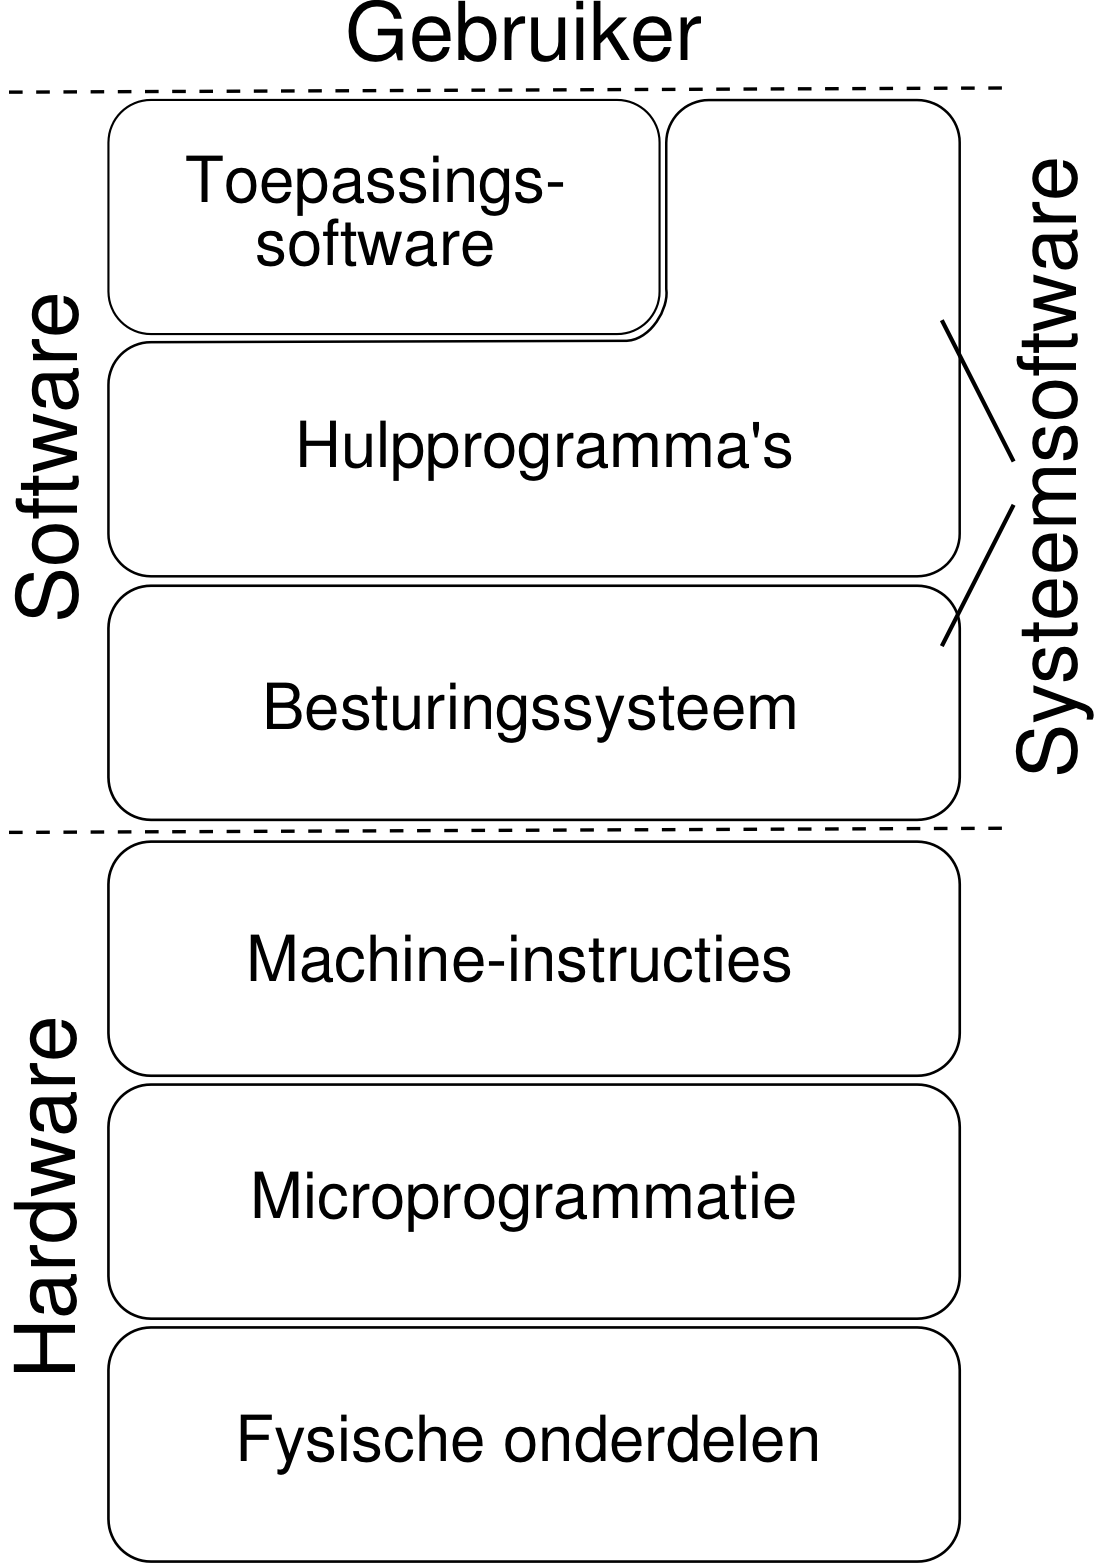
\includegraphics[width=60mm]{images/fig0101.png}
\end{center}
\caption{Situering}
\label{situering}
\end{figure}

\subsection{Hardware}

Men merkt hier een opsplitsing vooreerst in hardware en
software. De hardware zorgt voor de uitvoering van bevelen, die door
de software d.m.v. machine-instructies worden gegeven.

Deze instructies worden meestal niet rechtstreeks uitgevoerd
door de fysische onderdelen (chips, weerstanden, kabels enz.) maar via
een tussenlaag: de \emph{microprogrammatie} of
\emph{microcode}\index{microcode}. Dit is een verzameling van kleine
programma's in machinetaal die door de processoren worden begrepen en
toelaten dat relatief ingewikkelde operaties via \'e\'en
machine-instructie kunnen worden uitgevoerd. Microcode is een
voorbeeld van wat men firmware noemt: in ROM opgeslagen software. Men
vindt firmware vaak als enige softwarelaag terug in eenvoudigere
systemen met \'e\'en specifieke taak, zoals b.v. digitale camera's,
routers of GSM's. Het is bij deze toestellen over het algemeen niet
mogelijk extra software te installeren, maar soms is het wel mogelijk
om de firmware te vervangen door een nieuwe versie. Microcode heeft
niet \'e\'en specifieke taak, maar dient om het schrijven van programma's
in machinetaal te vereenvoudigen door vaak voorkomende taken aan te
bieden in \'e\'en oproep.

\subsection{Software}

De software kan worden opgesplitst in toepassingssoftware\index{toepassingssoftware} en
systeemsoftware\index{systeemsoftware}, die op zijn beurt bestaat uit het eigenlijke
besturingssysteem en een reeks hulpprogramma's.

Zonder de systeemsoftware is een computersysteem niet bruikbaar.
Het besturingssysteeem regelt de toegang tot de onderliggende
hardware. De hulpprogramma's worden aan het besturingssysteem
toegevoegd om het gebruik ervan te vergemakkelijken. Typische
voorbeelden zijn teksteditoren, compilers en programma's voor het
werken met bestanden.

Het uitvoeren van toepassingssoftware is het uiteindelijke doel
van het computersysteem. De enige bedoeling van de onderliggende lagen
is om dit mogelijk te maken. De hardware-lagen laten toe om
programma's in assembleertaal uit te voeren. Het besturingssysteem en
de hulpprogramma's dienen om dit zo effici\"ent en gemakkelijk mogelijk
te maken.

\section{Evolutie}

\subsection{Zonder besturingssysteem}

Bij de eerste computersystemen was nog geen sprake van een
besturingssysteem. Programma's werden in machinetaal geschreven, en de
computer kon maar 1 programma inladen en dan uitvoeren. Het laden en
starten gebeurde typisch door de programmeur zelf. Pas als een
programma afgelopen was kon het volgende geladen worden. Een programma
in uitvoering heeft in dit geval de volledige controle over alle
onderdelen van het computersysteem.

Na een tijd stelde men vast dat de geschreven programma's veel
gelijkaardige routines bevatten, b.v. voor in- en uitvoer. Ieder
programma moet gegevens inlezen, en moet op de een of andere manier
resultaten uitvoeren. Om te vermijden dat iedere programmeur deze
stukken machinecode opnieuw moest schrijven begonnen fabrikanten van
computersystemen \emph{bibliotheken} met vaak
gebruikte routines bij hun produkten te leveren. Een programmeur kon
zijn programma dan linken met code uit deze bibliotheken. Dit
vereenvoudigt het programmeren, maar de machine kan nog steeds maar
\'e\'en programma tegelijkertijd uitvoeren, en dit programma krijgt de
volledige controle over het systeem.

Bij het gebruik van de hierboven beschreven computersystemen
traden meer en meer planningsproblemen op. Er moest een planning
opgesteld worden om te bepalen wie de computer wanneer mocht
gebruiken. Als een programma vroeger dan voorzien klaar was, stond het
systeem stil tot de programmeur die het volgende tijdblok gereserveerd
had aankwam. Dat zo'n duur systeem tijdens dergelijke 'idle time'
ongebruikt blijft wilde men natuurlijk zo veel mogelijk vermijden.
Wanneer een programma langer moet rekenen dan voorzien ontstaat er ook
een probleem. Ofwel moet de volgende in de planning wachten, ofwel
moet het programma afgebroken worden en moet er nieuwe tijd
ingeroosterd worden. Bovendien bestaat de kans dat een programma door
een programmeerfout vastloopt. Het computersysteem wordt dan ook niet
gebruikt terwijl de programmeur de fout opspoort. Als de tijd op is
moet de programmeur opnieuw tijd inroosteren om het nog eens te
proberen.\footnote{Op dergelijke systemen was er nog geen sprake van
interactieve debuggers. Je kon je programma ook niet vlug even
aanpassen en opnieuw testen. Een programma moest bij iedere
wijziging opnieuw op ponskaarten gezet, ingeladen en uitgevoerd
worden. Er wordt wel eens gezegd dat de hedendaagse
informatica-studenten slechtere of alleszins minder zorgvuldige
programmeurs zouden zijn door het toegenomen
gebruiksgemak...}

\subsection{Een mens als besturingssysteem!?}

Om de planningsproblemen te ondervangen werd na verloop van tijd
een \emph{menselijke operator} ge\"introduceerd.
Programmeurs brengen de uit te voeren programma's naar de operator, op
ponskaarten, papierband of magneetband. Het laden en starten van de
verschillende programma's is nu de taak van de operator. Hierdoor zijn
de problemen met de planning grotendeels opgelost. De operator
bezorgt de programmeur het resultaat van zijn programma, of eventueel
de inhoud van het geheugen op het moment dat er een fout optrad. Met
deze zogenaamde \emph{core dump}\footnote{De term core dump is
afgeleid van magnetic core memory, \'e\'en van de eerste types computergeheugen.
Zie b.v. \url{http://en.wikipedia.org/wiki/Core_memory}}
kan de programmeur dan op zoek naar de fout.

Er ontstaan ook extra mogelijkheden doordat de programma's
aangeleverd worden, en dan door de operator gestart worden. Er kunnen
prioriteiten toegekend worden aan verschillende programma's. De
operator kan hiermee rekening houden bij het bepalen van de volgorde
waarin de programma's gestart worden. Hij moet niet noodzakelijk de
volgorde waarin ze aangeleverd worden respecteren. De operator kan ook
gegevens bijhouden, b.v. de gebruikte computertijd per programma. Met
deze gegevens kan het gebruik van het computersysteem eventueel
gefactureerd worden aan de gebruikers. Later werden meer gegevens
genoteerd, zoals het aantal geprinte pagina's, ingelezen ponskaarten,
operator-interventies, hoeveelheid gebruikte schijfruimte, ...

Computersystemen worden steeds sneller, maar de menselijke
operatoren niet. Hierdoor worden zij meer en meer de vertragende
factor. Als een operator 10 seconden nodig heeft om een programma te
starten, en het programma duurt 90 seconden, dan gaat er 10\% van de
tijd naar de operator. Als de computer 3 keer sneller wordt, is het
programma voltooid na 30 seconden. De totale tijd wordt 40 seconden,
en het aandeel van de operator is al goed voor 25\%.

Bovendien laten de krachtigere systemen, waarvan ook de
opslagcapaciteit blijft toenemen, toe dat de door de fabrikant
meegeleverde bibliotheken alsmaar meer en complexere taken vervullen.
Zo kunnen ze de facturatiegegevens bijhouden, en het volgende
programma starten. Zo wordt de vertraging van de menselijke operator
gedeeltelijk weggewerkt. Als de bibliotheken ook nog proberen te
voorkomen dat er misbruik gemaakt wordt van de beschikbare
hulpmiddelen van het systeem, kunnen we stellen dat ze evolueren naar
de eerste besturingssystemen.

\subsection{De eerste besturingssystemen}

We kunnen eigenlijk pas van een besturingssysteem spreken vanaf
het moment dat de zogenaamde \emph{residente monitors}\index{monitor}
gebruikt worden, omdat zo'n residente monitor instaat voor de controle
van het systeem, \'en constant in het geheugen gehouden worden (vandaar
'resident').

De residente monitor wordt gedurende de ganse werkperiode van de
computer in het geheugen gehouden en zorgt ervoor dat een uit te
voeren programma in het geheugen wordt geladen en gestart. Daartoe
wordt een sprong uitgevoerd naar het beginadres van het programma, en
wordt aan het einde van het programma een sprong naar de monitor
toegevoegd. Zo kan de monitor het computersysteem voortdurend
controleren, eventueel in samenspraak met de operator. De operator
moet wel nog steeds zorgen voor het aanbieden van de uit te voeren
programma's, maar de rest van het beheer is overgenomen door de
residente monitor.

Uit de codebibliotheken die bij de computersystemen geleverd
worden evolueren ook specifieke besturingsroutines voor randapparaten,
\emph{device drivers} genoemd. Door deze drivers wordt
het geven van opdrachten aan en het communiceren met randapparatuur
eenvoudig. Een programma moet gewoon de juiste functie van de driver
aanroepen. Wanneer je programma gebruik moest maken van een ander type
randapparaat, moest je nu enkel nog de oproep van de device driver
aanpassen. Samen met de opkomst van de hogere programmeertalen zorgden
de device drivers dat het voor veel meer ge\"interesseerden mogelijk
werd om computers te gebruiken.

Deze eerste besturingssystemen groeien uit tot eenvoudige
\emph{batch-besturingssysteem}.\index{batch-systeem} De term batch (groep,
verzameling) wijst op de gebruikswijze van dit soort systemen: men
biedt een stel programma's als een globaal pakket aan het
besturingssysteem aan en deze programma's worden dan onder controle
van dit systeem en zonder verdere tussenkomst van een gebruiker of
operator \'e\'en na \'e\'en uitgevoerd.

\subsection{Multiprogrammatie en Time Sharing}\index{multiprogrammatie}\index{time sharing}

Batch-besturingssystemen kennen een steeds groter wordend
effici\"entie-probleem. Terwijl het programma dat ze aan het uitvoeren
is, wacht op het voltooien van in- of uitvoer, wordt de processor van
het computersysteem niet gebruikt. Bovendien nam het belang van deze
perioden van inactiviteit toe naarmate de processoren sneller
werden.

Als oplossing worden de besturingssystemen uitgebreid met
\emph{multiprogrammatie}\index{multiprogrammatie}. Terwijl een programma moet
wachten op een externe gebeurtenis laat het besturingssysteem de
processor verderwerken aan een ander programma. Dit leidt tot een
situatie waarin een reeks verschillende programma's samen in het
geheugen aanwezig zijn en om de beurt worden uitgevoerd tot ze moeten
wachten. Het lijkt dan alsof de computer al deze programma's tegelijk
uitvoert, maar de processor is altijd maar met \'e\'en van de programma's
bezig.

Wanneer een multiprogrammatie-systeem wordt uitgebreid met een
\emph{spooling}-systeem\index{spooler} (SPOOL: Simultaneous
Peripheral Operation OnLine), dat een aantal jobs kan klaarhouden op
een snel extern geheugen en de simultane\footnote{Zoals gezegd is deze simultane
uitvoer slechts schijn, de computer werkt eigenlijk om de beurt aan de
verschillende programma's, maar het probleem is wel re\"eel. Als deze
programma's b.v. regelmatig een lijn naar een printer sturen is het natuurlijk
niet de bedoeling dat de uitvoer naar de printer van beide programma's op
\'e\'en blad vermengd wordt.} uitvoer (output) van verschillende jobs op een
ordelijke manier kan afhandelen komt men tot een zeer krachtig
besturingssysteem.

De multiprogrammatie-systemen kenden nog een groot gebrek: het
gebrek aan interactiviteit. Het is nog steeds zo dat men een programma
laat uitvoeren en dan wacht op het resultaat. Als dat resultaat niet
is wat men verwachtte, moet men het programma wijzigen en opnieuw
laten uitvoeren. De schijnbaar simultane uitvoer van programma's bij
multiprogrammatie laat ook toe om verschillende gebruikers tegelijk op
een interactieve wijze met een computer te laten werken. Elke
gebruiker beschikt dan over een in- en uitvoerapparaat, verbonden met
de centrale verwerkingseenheid, dat hem toelaat met de computer te
communiceren. Omdat de processor afwisselend gedurende korte tijd aan
elke gebruiker wordt toegewezen krijgt elk van hen de indruk
voortdurend te beschikken over alle faciliteiten van het
computersysteem. Deze vorm van multiprogrammatie wordt \emph{time
sharing} genoemd.\index{time sharing} Het belangrijkste verschil met de
hierboven beschreven multiprogrammatie is dat er bij time sharing niet
gewacht wordt tot een programma moet wachten om de processor aan een
ander programma toe te kennen.

Doordat de gebruiker op een time sharing systeem rechtstreeks
met de computer kan communiceren, krijgt hij bijna onmiddellijk
feedback bij kleinere opdrachten. Hierdoor neemt het gebruikscomfort
sterk toe. Doordat gebruikers typisch niet tegelijkertijd pieken
veroorzaken in het processorgebruik lijkt het systeem voor ieder van
hen toch performant te werken. Je zou kunnen zeggen dat de computer de
invoer meestal sneller kan verwerken dan de gebruiker ze kan
genereren. Hierdoor kan de computer meerdere gebruikers tegelijk
bedienen. Voor het accepteren van invoer via een toetsenbord moet de
processor zeer weinig werk verrichten, dus terwijl de ene gebruiker
een opdracht typt, is er processorkracht over voor het inlezen van de
toetsenborden van andere gebruikers, of het werken aan eerder gegeven
opdrachten. Als er dan nog processorkracht over is, kan eventueel nog
steeds aan niet-interactieve batch-verwerking van opdrachten gedaan
worden. Als er veel interactief gebruik is moeten de batch-taken
wachten.

\subsection{Besturingssystemen voor Minicomputers}

In de jaren 60 kwamen de \emph{minicomputers}\index{minicomputer} op
de markt. Laat je niet misleiden, zo'n minicomputer was 'mini' omdat
hij maar enkele kasten in beslag nam terwijl de eerdere systemen een
volledige kamer in beslag namen. Tot dan had men gewoon van computers
gesproken, maar nu werden de grotere modellen mainframes genoemd.\index{mainframe} Men
zegt ook soms dat de minicomputers de eerste computers waren die door
\'e\'en persoon bediend konden worden.

Bij mainframes was het de gewoonte dat een fabrikant een
besturingssysteem ontwikkelde telkens hij een nieuw model op de markt
bracht. Dit was voor de fabrikant een zware inspanning, maar voor de
gebruiker betekende het ook telkens grote conversieproblemen als er
naar een nieuwere en krachtigere computer overgeschakeld werd. Al de
programma's moesten namelijk aangepast worden aan het nieuwe
besturingssysteem.

In 1964 lanceerde IBM voor het eerst een familie van
computersystemen. De System/360 reeks van mainframes omvatte modellen
met verschillende verwerkingscapaciteiten, maar ze waren allemaal
gebaseerd op dezelfde architectuur. Dit liet toe op al deze modellen
hetzelfde besturingssysteem te gebruiken en betekende dat bij het
overgaan naar een ander model van dezelfde reeks bijna alle
conversieproblemen verdwenen. Alle modellen gebruikten dan ook (een
variant van) hetzelfde besturingssysteem: OS/360. Omdat OS/360 voor
allerlei soorten toepassingen moest gebruikt worden, werd het een zeer
ingewikkeld besturingssysteem. Deze systemen werden soms
multimode-systemen genoemd omdat ze zoveel verschillende werkwijzen
moesten aankunnen.

Door de opkomst van de minicomputers groeide de markt voor
computersystemen. Door deze stijging van het aantal computergebruikers
ging er meer aandacht naar de gebruiksvriendelijkheid en de
interactiviteit van de besturingssystemen. De PDP's (Programmed Data
Processor) van Digital Equipment waren een zeer succesvolle reeks van
minicomputers. De PDP-1 kwam op de markt in 1961. Voor
\$120.000\footnote{Dit zijn "1960 dollars", wat zou overeenkomen
met meer dan 700.000 hedendaagse dollars. Dit lijkt veel, maar voor een gewone
mainframe betaalde je in 1960 al gauw \$1.000.000 (ook "1960 dollars")} had je
een machine met een geheugencapaciteit van 4000 woorden van 18 bits, m.a.w. 9
kilobyte. Een andere vroege minicomputer was de LINC, ook van DEC. Figuur \ref{linc_specs} toont de specificaties van de LINC uit de oorspronkelijke brocure uit 1961. Figuur \ref{linc_prijs} toont een prijslijst.

\begin{figure}
\begin{center}
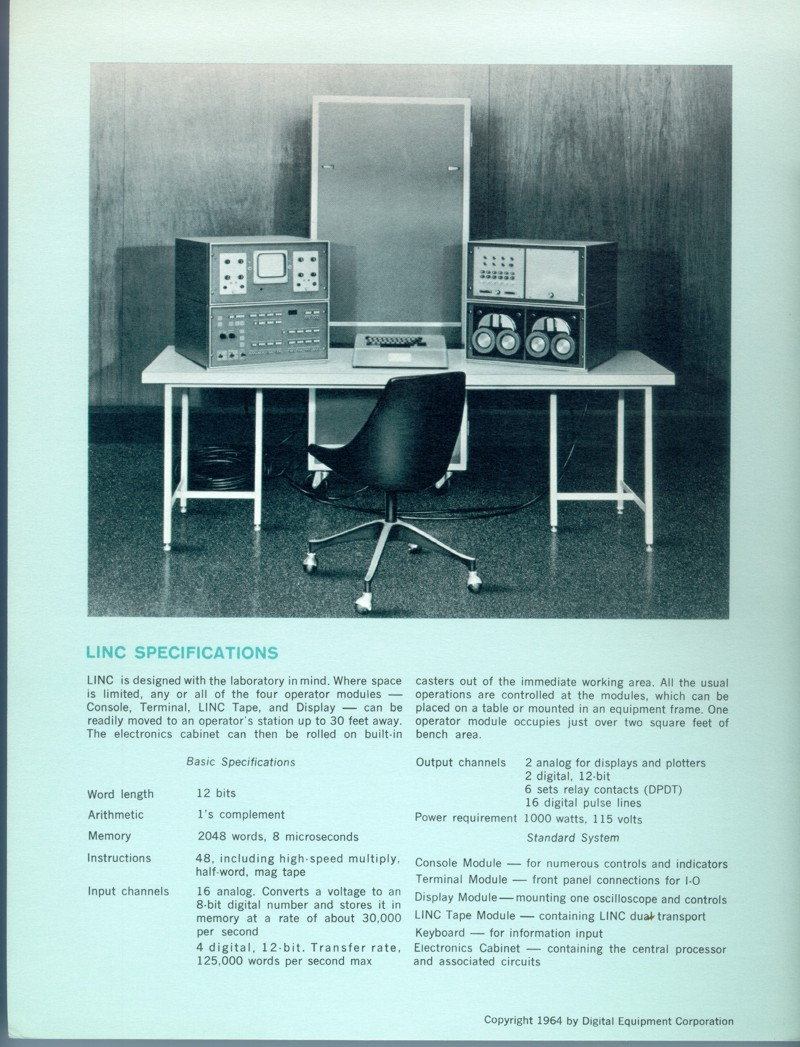
\includegraphics[width=\textwidth]{images/linc01.jpg}
\end{center}
\caption{LINC Specificaties}
\label{linc_specs}
\end{figure}

\begin{figure}
\begin{center}
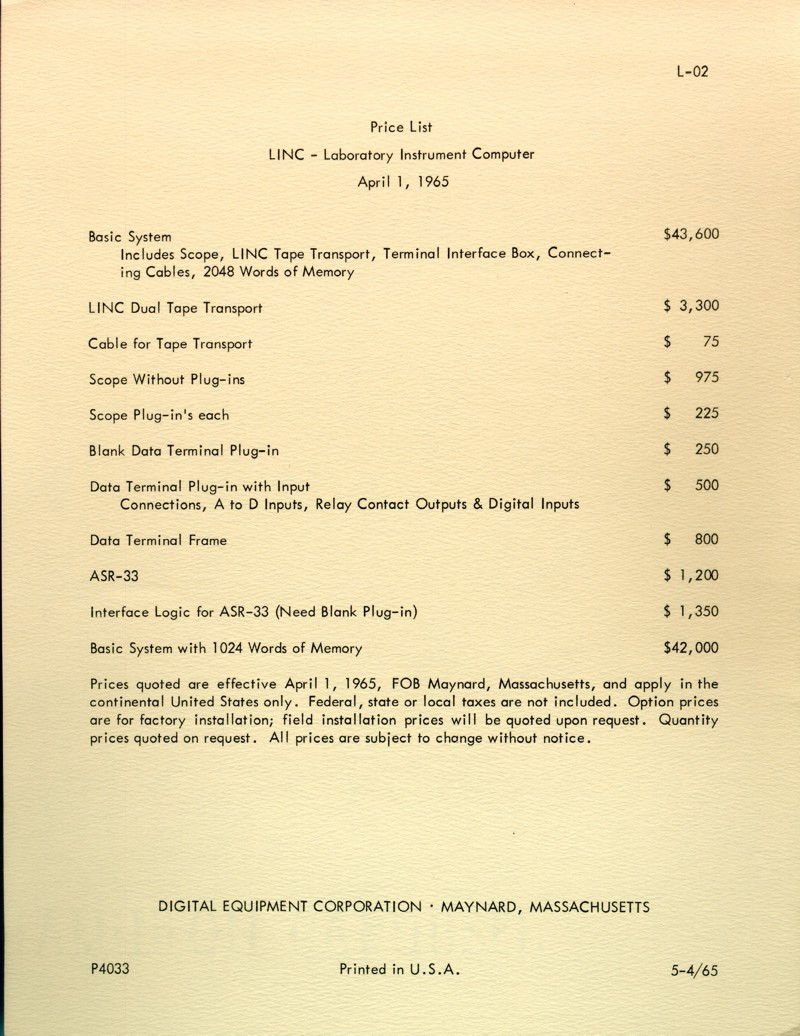
\includegraphics[width=\textwidth]{images/linc02.jpg}
\end{center}
\caption{LINC Prijslijst}
\label{linc_prijs}
\end{figure}

In de wetenschappelijke wereld raakte intussen stilaan
\emph{UNIX}\index{besturingssysteem!UNIX} bekend, een nieuw besturingssysteem dat
niet door een computerconstructeur werd ontwikkeld en waar (althans
oorspronkelijk) geen commerci\"ele bedoelingen aan vastzaten. Het was
een klein besturingssysteem met multiprogrammatie en ondersteuning
voor meerdere gebruikers. De belangrijkste nieuwigheid was dat het,
mits enkele kleine aanpassingen, op elke hardware bruikbaar kon worden
gemaakt en daarbij naar de gebruiker toe steeds dezelfde interface
bood. Dit was ondermeer te danken aan het feit dat het niet in een
assembleertaal, maar in een daarvoor speciaal ontwikkelde hogere
programmeertaal, C genaamd, was geschreven. De ontwikkeling van UNIX
wekte voor het eerst de hoop op een standaard-besturingssysteem en
probleemloos uitwisselbare toepassingssoftware.

\subsection{De PC en het Internet}

Wat men van UNIX verwachtte werd in de jaren 80 vrij onverwacht
gerealiseerd, zij het op een totaal andere manier. Aan het eind van
de jaren 70 dook de microcomputer op. Toen IBM zijn
\emph{microcomputer}\index{microcomputer}, de Personal Computer of PC,
lanceerde en hiervoor een nieuw besturingssysteem, MS-DOS\index{besturingssysteem!MS-DOS}, liet
ontwikkelen bleek dit zo'n groot succes dat de meeste andere
constructeurs deze architectuur overnamen. Hierdoor ontstond een
enorme markt met uniforme computers: de IBM-compatibele PC's. Men kon
nu toepassingssoftware ontwikkelen die op zowat 90\% van de zich
massaal verspreidende microcomputers kon worden gebruikt.

De grote verspreiding van de microcomputer zorgde ervoor dat
eigenlijk iedereen met een computer wou gaan werken. Hierdoor moest er
dringend werk gemaakt worden van een vereenvoudiging van de
gebruikersinterface. Vandaar de ontwikkeling van GUI's (Graphical User
Interfaces), waarmee op een symbolische manier bevelen aan de computer
konden worden gegeven. In 1984 kwam de Apple Macintosh SE op de markt,
de eerste computer met een GUI. De SE kostte \$2495, en bevatte een 8
MHz processor en een werkgeheugen van 4 MB. In 1985 was er dan de
eerste versie van Windows\index{besturingssysteem!Windows}, een grafische laag bovenop MS-DOS. Een GUI
is een mooi voorbeeld van een hulpprogramma dat bij het eigenlijke
besturingssysteem zit om het gebruik ervan te vereenvoudigen.

De stijgende performantie van de microcomputer was ideaal voor
multitasking: time sharing voor \'e\'en gebruiker. De gebruiker kan
verschillende opdrachten tegelijk laten uitvoeren, en deze opdrachten
laten samenwerken. De processortijd wordt door het besturingssysteem
verdeeld over al de opdrachten.

De gebrekkige communicatie tussen computers was het volgende
obstakel. Dit leidde tot het introduceren van netwerken. Eerst LANs,
daarna WANs en uiteindelijk de wereldwijde verbindingen tussen al deze
netwerken. Het geheel kennen we nu als het Internet.

\section{Voorbeelden van Besturingssystemen}

Bij het bespreken van de evolutie van besturingssystemen kwamen al
enkele voorbeelden aan bod zoals OS/360 en MS-DOS. Aangezien
besturingssystemen sinds OS/360 niet meer specifiek voor \'e\'en bepaalde
machine ontworpen worden, zijn ze nu meestal verbonden met \'e\'en van de
drie besproken types: mainframes, minicomputers of
microcomputers.

Doordat iedereen nu over een PC beschikt lijkt het misschien alsof
mainframes afgedaan hebben, maar dat blijkt niet het geval. IBM is nog
steeds \'e\'en van de grote spelers in de mainframe-markt, en er worden nog
steeds mainframes ontwikkeld. De S/360 reeks is ge\"evolueerd naar de
S/370 en later de S/390 reeks. Nu worden de IBM mainframes zSystems
genoemd. De besturingssystemen die in de loop der jaren voor deze
systemen ontwikkeld zijn omvatten klinkende namen als MVS, VM en
VSE.

Ook minicomputers zijn nog steeds te verkrijgen en in gebruik. Men
spreekt nu ook soms van midrange systemen, en IBM noemt ze iSeries. In
de jaren 80 waren er twee grote concurrenten in dit marktsegment. Digital
(later Compaq en nu HP) had de VAX-machines, met als besturingssysteem
VMS, en OS/400 op de IBM AS/400 computers.

Voor microcomputers waren er in de jaren 80 drie families. Op
IBM-compatibele PC's had je de keuze tussen MS-DOS van Microsoft en OS/2
van IBM. Voor Macintosh computers was er System 7. OS/2 is van de markt
verdwenen, en MS-DOS is ge\"evolueerd naar de verschillende versies van
Windows. Windows was eerst slechts een grafische toevoeging aan MS-DOS,
maar de recentere versies zijn volledige besturingssystemen. Voor
Macintosh computers heb je tegenwoordig MacOS nodig.

Er zijn ook besturingssystemen die niet aan \'e\'en van de 3 grote
categorie\"en van computersystemen verbonden zijn. Ze kunnen in principe
op iedere computer worden gebruikt. Allereerst is er UNIX dat men op de
meest diverse hardware aantreft, zij het in allerlei varianten. Op
mainframes vind je AIX (IBM) als gast onder VM. Op VAX minicomputers
werd Ultrix (later Digital Unix) gebruikt terwijl voor microcomputers
SCO Unix (vroeger Xenix) of HPUX beschikbaar is. Voor PC's (maar ook
voor andere platformen) is er sinds 1991 ook het steeds populairdere
GNU/Linux.

In deze cursus zullen we vooral Windows en Linux als voorbeeld
gebruiken.

\section{Functies van een besturingssysteem}

Zoals reeds aangehaald heeft het besturingssysteem twee grote
taken: het \emph{gebruiksgemak} en de
\emph{effici\"entie} van het computersysteem maximaliseren.
Naar de gebruiker toe proberen we b.v.:

\begin{description}
\item[De toegang tot apparaten eenvoudig te maken]Toepassingssoftware moet b.v.
op een eenvoudige manier in- en uitvoerapparaten kunnen aanspreken. Device
drivers laten toe abstractie te maken van de specifieke hardware.
\item[Informatie bewaren en overzichtelijk weergeven]Gebruikers willen hun
gegevens opslaan en later terug ophalen. Het besturingssysteem moet opslagmedia
zoals harde schijven bruikbaar maken.
\item[Operaties en gegevens beveiligen]Gegevens van verschillende gebruikers of
programma's moeten afgeschermd worden van andere gebruikers of programma's.
\end{description}

Wat betreft de hardware wordt er getracht:

\begin{description}
\item[De onderlinge communicatie tussen onderdelen te organiseren]
\item[De goede werking van de onderdelen bewaken]Wanneer er een fout optreedt in
de hardware moet die gedetecteerd en zo mogelijk gecorrigeerd worden.
\item[Hulpmiddelen rechtvaardig te verdelen]Verschillende gebruikers en
programma's willen gebruik maken van de aanwezige hulpmiddelen, en het
besturingssysteem staat in voor de verdeling.
\end{description}

Merk op dat het besturingssysteem ook een programma is dat door de
processor uitgevoerd moet worden. De gebruiker van een systeem wil
alleen zijn software uitvoeren, en niet het besturingssysteem. We kunnen
dus stellen dat de tijd dat het besturingssysteem de processor gebruikt
verloren gaat voor de gebruiker. Effici\"entie is dus een belangrijke
vereiste voor het besturingssysteem, om de hoeveelheid overhead te
beperken. Het is belangrijk te beseffen dat, hoewel het in theorie om
onnuttige processortijd gaat, het besturingssysteem ervoor zou moeten
zorgen dat de computer beter gebruikt wordt. Enerzijds wordt de computer
gemakkelijker om te gebruiken, en anderzijds ontstaan er mogelijkheden
die er zonder besturingssysteem niet zouden zijn, zoals het uitvoeren
van meerdere programma's tegelijkertijd.

Een derde taak voor het besturingssysteem is om te streven naar
\emph{hardware-onafhankelijkheid}. Als het
besturingssysteem een uniforme interface aanbiedt aan de de
bovenliggende toepassingssoftware en de gebruiker kan de hardware
aangepast worden zonder overgangsproblemen, zoals ge\"illustreerd in
figuur \ref{platform}. In de bespreking van de evolutie van
besturingssystemen zijn we hiervan al enkele voorbeelden tegengekomen.
De eerste stap naar hardware-onafhankelijkheid was de introductie
van device drivers.

\begin{figure}
\begin{center}
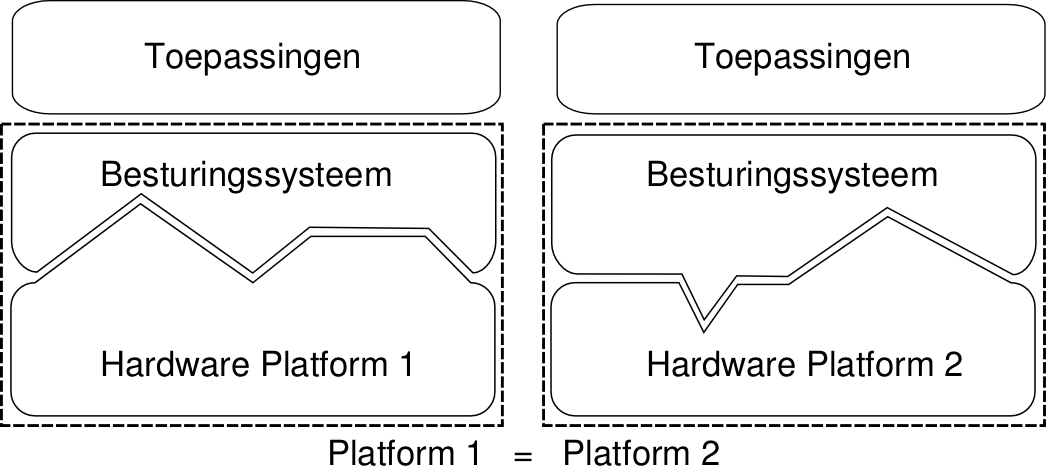
\includegraphics[width=80mm]{images/fig0102.png}
\end{center}
\caption{Besturingssysteem zorgt voor hardware-onafhankelijkheid}
\label{platform}
\end{figure}

Er zijn versies van de Linux-kernel voor verschillende
architecturen, b.v. x86, Alpha, SPARC, ARM en S/390. Toepassingssoftware
die geschreven is voor de Linux-kernel kan dus op ieder van deze
architecturen uitgevoerd worden.

\section{Taken van een besturingssysteem}

In het vervolg van deze cursus wordt de werking van een besturingssysteem
meer in detail bekeken. Een besturingssysteem heeft verschillende taken, en
de ontwerpers van een besturingssysteem moeten rekening houden met soms
tegenstrijdige doelstellingen.

\subsection{Bestandsbeheer}

Op opslagmedia zoals b.v. magneetschijven kunnen enen en nullen
weggeschreven worden. Omdat dit niet handig is bieden de meeste
besturingssystemen de gebruiker de mogelijkheid om met bestanden te
werken. Het besturingssysteem zal deze bestanden dan op de
schijf opslaan en ze terug inlezen wanneer de gebruiker daarom vraagt.
Bovendien zal ook rekening gehouden moeten worden met aspecten zoals
toegangscontrole en optimaal gebruik van beschikbare
schijfruimte.

\subsection{Apparaatbeheer}

De toegang tot de randapparatuur moet door het besturingssysteem
geregeld worden, om b.v. conflicten te vermijden. Als 2 programma's
tegelijkertijd naar de printer zouden kunnen schrijven zouden we
vreemde resultaten krijgen.

\subsection{Geheugenbeheer}

Computerprogramma's kunnen niet uitgevoerd worden zonder toegang
tot werkgeheugen, maar ook hier komt enige organisatie aan te pas.
Programma's mogen b.v. niet in elkaars geheugensegmenten lezen of
schrijven. Aangezien het beschikbare werkgeheugen beperkt is moet het
besturingssysteem ook streven naar effici\"ent gebruik ervan.

\subsection{Procesbeheer}

Procesbeheer omvat in essentie het verdelen van de beschikbare
processortijd over de verschillende processen die uitgevoerd moeten
worden. Hier wordt gezorgd voor multiprogrammatie en
multitasking.

\subsection{Communicatie}

Het besturingssysteem staat in voor de communicatie tussen
processen op het computersysteem, maar ook voor eventuele communicatie
met andere computersystemen via een netwerk.

\subsection{Gebruikersinterface}

Om het gebruik van de computer te vereenvoudigen moet het
besturingssysteem ook zorgen voor een adequate gebruikersinterface.
Dit kan een tekstgebaseerde interface aan een commandoprompt zijn,
maar ook een grafische omgeving is mogelijk. Deze taak hangt samen met
al de andere, omdat de gebruiker natuurlijk een interface nodig heeft
om het bestandssysteem aan te spreken.

\subsection{Veiligheid}

Het besturingssysteem beschermt de onderdelen van het computersysteem tegen
onrechtmatig gebruik. Zo mogen enkel gekende gebruikers toegang krijgen tot
het systeem, en enkel tot die delen van het systeem waar ze rechten op hebben.
Ook verschillende programma's die uitgevoerd worden moeten van mekaar
afgeschermd worden.

\chapter{Basismechanismen van een besturingssysteem}\label{chap:basis}

\section{Kernel- en gebruikerstoestand}

Kenmerkend voor het besturingssysteem is dat de programma's, die
er deel van uitmaken, worden uitgevoerd in
\emph{kernel-toestand}\index{kernel mode}\index{supervisor mode}\index{monitor-toestand} (kernel mode, ook wel supervisor-
of monitor-toestand genoemd). Hiermee duidt men een bijzondere toestand
aan van de processor. Wanneer de processor zich in kernel-toestand
bevindt, beschikt hij over al zijn mogelijkheden. Wanneer de processor
niet in kernel-toestand is, maar in
\emph{gebruikerstoestand} (user mode)\index{gebruikerstoestand (user mode)}, zijn bepaalde
instructies niet toegelaten.

Tussen de machine-instructies, ingebouwd in de processor, zijn er
namelijk een aantal die men \emph{geprivilegieerde instructies}\index{gepriviligeerde instructie}
noemt. Deze laatste (b.v. instructies voor I/O, voor het
reserveren van geheugenruimte, om de toestand van de processor te
wijzigen enz.) kunnen alleen worden uitgevoerd in kernel-toestand en
zijn daardoor voorbehouden aan het besturingssysteem. De
toepassingssoftware en de overige systeemsoftware worden immers
uitgevoerd in gebruikerstoestand. Wanneer een programma probeert om in
gebruikerstoestand een geprivilegieerde instructie uit te voeren zal een
fatale fout optreden, en het betrokken programma zal be\"eindigd
worden.

Op die manier kunnen allerlei delicate operaties op een
gegarandeerd veilige manier worden uitgevoerd. Ze kunnen namelijk enkel
door het besturingssysteem uitgevoerd worden, waardoor het in staat is
om de omstandigheden waarin deze operaties plaatsvinden volledig te
controleren. Wanneer het besturingssysteem een gewoon programma laat
uitvoeren zal het de processor eerst naar gebruikerstoestand brengen
alvorens het programma te starten (door een sprong). In de
toestandsbeschrijving van de processor is een bit voorzien om de
toestand aan te geven waarin deze zich bevindt: user mode of kernel
mode.

\section{Interrupts}

Een besturingssysteem mag niet worden gezien als een soort
superprogramma, dat voortdurend alle activiteiten in het computersysteem
van boven af regelt. Het komt in tegendeel slechts in actie na een
signaal vanuit de hardware of na een vraag vanuit de toepassingssoftware.
Men zegt dan ook dat een besturingssysteem \emph{gebeurtenisgestuurd},
of \emph{event driven} is.

\begin{figure}
\begin{center}
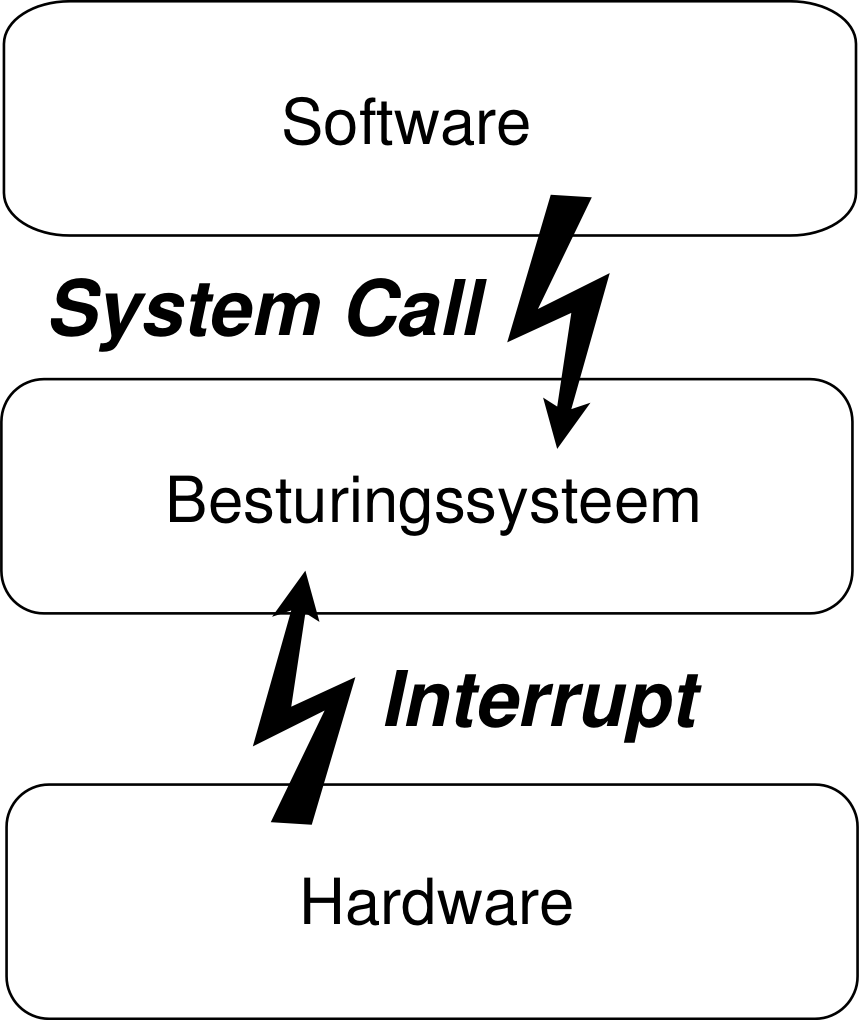
\includegraphics[width=50mm]{images/fig0201.png}
\end{center}
\caption{System calls en interrups}
\label{sysint}
\end{figure}

\subsection{Interrupt requests}

Wanneer vanuit de hardware behoefte is aan een tussenkomst van
het besturingssysteem treedt een \emph{interrupt request}\index{interrupt request} of
\emph{onderbrekingsaanvraag} op. Dit zijn in feite berichtjes die de hardware naar de processor kan sturen wanneer er \emph{iets} gebeurt. De processor ziet dat er een berichtje binnengekomen is, gaat dan de actieve applicatie onderbreken en springt naar code van het besturingssysteem om de interrupt request af te handelen. Wanneer er niets gebeurt komen er geen interrupt requests binnen, en kan de processor volledig gebruikt worden voor het uitvoeren van het actieve programma.

Voor het genereren en afhandelen van interrupt requests is de nodige hardwareondersteuning nodig. Zo moet er bijvoorbeeld bepaald worden wanneer de processor kijkt of er een interrupt request binnengekomen is en hoe die dan afgehandeld moet worden.

In het vak Computersystemen werd uitvoerig uitgelegd hoe de processor instructies verwerkt. Er werd gezegd dat er twee fases zijn: de \emph{haalcyclus} en de \emph{uitvoeringscyclus}. In de haalcyclus werd een bevel opgehaald, en in de uitvoeringscyclus werd het opgehaalde bevel dan uitgevoerd. Na de uitvoeringscyclus gaat de processor terug naar de haalcyclus om het volgende bevel op te halen, enz. Figuur~\ref{fig:nointerrupts} geeft schematisch weer hoe dit proces werkt.

\begin{figure}
  \centering
  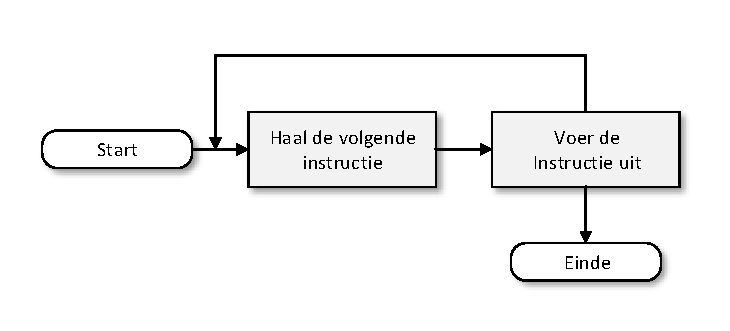
\includegraphics[scale=0.8]{images/NoInterrupts.pdf}
  \caption{Een processor zonder interrupt-ondersteuning.}\label{fig:nointerrupts}
\end{figure}

Wanneer een processor echter het concept van interrupts ondersteunt, wordt het verhaal iets ingewikkelder. Er moet nu namelijk ook regelmatig gecontroleerd worden of er een interrupt request binnengekomen is. Uiteindelijk komen we dan tot het resultaat in figuur~\ref{fig:withinterrupts}. De processor voert nog altijd een haalcyclus en dan een uitvoeringscyclus uit, maar gaat daarna eerst controleren of er een interrupt request binnengekomen is. Indien dit niet het geval is, gaat de processor naar de volgende haalcyclus. Ook indien de afhandeling van interrupt requests (tijdelijk) afgezet is, zal de processor rechtstreeks van de uitvoeringscyclus naar de volgende haalcyclus gaan. In het geval dat er echter wel een interrupt request binnengekomen is, zal de processor de afhandeling van van die interrupt request opstarten (de afhandeling van een interrupt request noemen we \emph{een interrupt}\index{interrupt}).

\begin{figure}
\centering
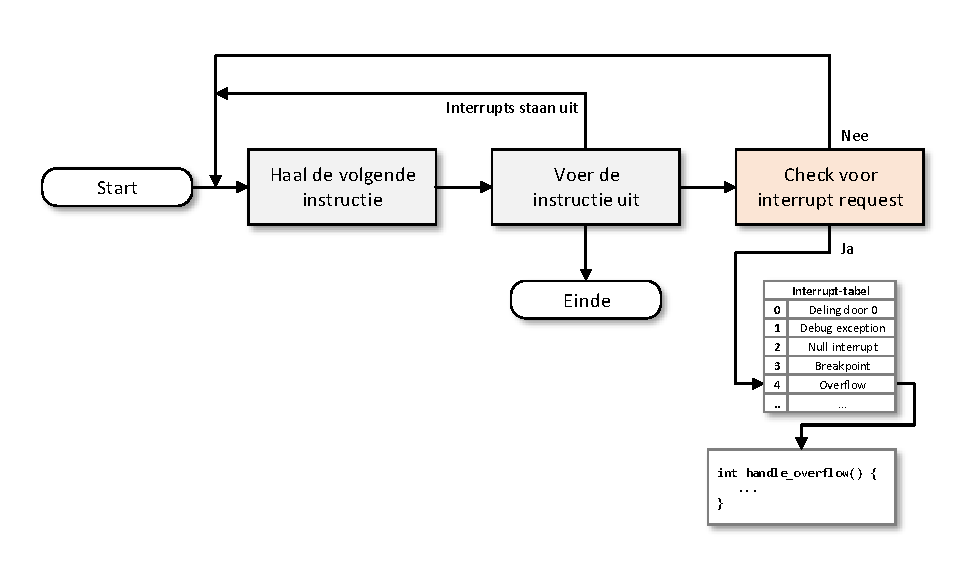
\includegraphics[scale=0.8]{images/WithInterrupts.pdf}
\caption{Een processor met interrupt-ondersteuning.}\label{fig:withinterrupts}
\end{figure}

\subsection{Interrupt requests afhandelen}

Een interrupt request is een elektrisch signaal naar de processor, of
een gebeurtenis binnenin de processor zelf. Als de harde schijf b.v.
een leesopdracht voltooid heeft, zal de schijfbesturingseenheid dit
via een interruptsignaal naar de processor aan het besturingssysteem
melden. Binnen de processor zou een interrupt request kunnen optreden wanneer
een programma deelt door nul, of wanneer een programma een
geprivilegieerde (en dus niet toegelaten) instructie gebruikt.

Deze verschillende types van interrupts moeten allemaal op andere manieren behandeld worden. Om het een en ander te vereenvoudigen bestaat er een \emph{interrupttabel}\index{interrupttabel} die voor elk type interrupt een geheugenadres van een methode bijhoudt die opgeroepen moet worden wanneer een overeenkomstige interrupt request binnenkomt.

Op de Intel x86-processor bestaat de interrupttabel uit 256 waardes (ook wel \emph{interrupt vectors}\index{interrupt vector} genoemd). De eerste 32 waardes zijn gereserveerd voor Intel en worden gebruikt om processorfouten af te handelen. De overige waardes kunnen ingesteld worden door het besturingssysteem, afhankelijk van de hardware die aanwezig is in het systeem. Als er bijvoorbeeld een netwerkkaart aanwezig is, kan het besturingssysteem bijvoorbeeld het interrupt nummer 97 toekennen aan die kaart (eender welk vrij nummer kan natuurlijk gekozen worden). Wanneer die netwerkkaart dan een netwerkpakketje binnenkrijgt, moet het een interrupt request met waarde 97 sturen naar de processor. Zo weet het besturingssysteem dat de interrupt van de netwerkkaart komt. Een overzicht vind je in figuur~\ref{table:ivt}.

\begin{figure}
\centering
\begin{tabular}{|c|l|}
  \hline
  \textbf{Interrupt nummer} & \textbf{Beschrijving (Engels)} \\
  \hline
  0 & divide error \\
  1 & debug exception \\
  2 & null interrupt \\
  3 & breakpoint \\
  4 & overflow \\
  5 & bound range exception \\
  6 & invalid processor instruction \\
  7 & device not available \\
  8 & double fault \\
  9 & coprocessor segment overrun \\
  10 & invalid task state segment \\
  11 & segment not present \\
  12 & stack fault \\
  13 & general protection \\
  14 & page fault \\
  15 & (Intel reserved, do not use) \\
  16 & floating-point error \\
  17 & alignment check \\
  18 & machine check \\
  19-31 & (Intel reserved, do not use) \\
  32-255 & maskable interrupts \\
  \hline
\end{tabular}
\caption{De inhoud van de Intel x86 interrupttabel.}
\label{table:ivt}
\end{figure}

Wanneer er een interrupt binnenkomt, gaat de processor de juiste entry van de interrupttabel opvragen en daar naartoe springen. Figuur~\ref{fig:withinterrupts} toont bijvoorbeeld de afhandeling van een overflowfout (d.i. interrupttype 4). Wanneer die fout zich voordoet gaat de processor in de interrupttabel de interrupt vector op plaats 4 opvragen. Deze verwijst dan door naar de methode \emph{handle\_overflow} die een deel is van het besturingssysteem en de fout afhandelt. Zulke methodes noemen we ook wel \emph{interrupt service routines}.

Laten we het voorbeeld van de leesopdracht voor de harde schijf
even bekijken (figuur \ref{lezenhd}).

\begin{figure}
\begin{center}
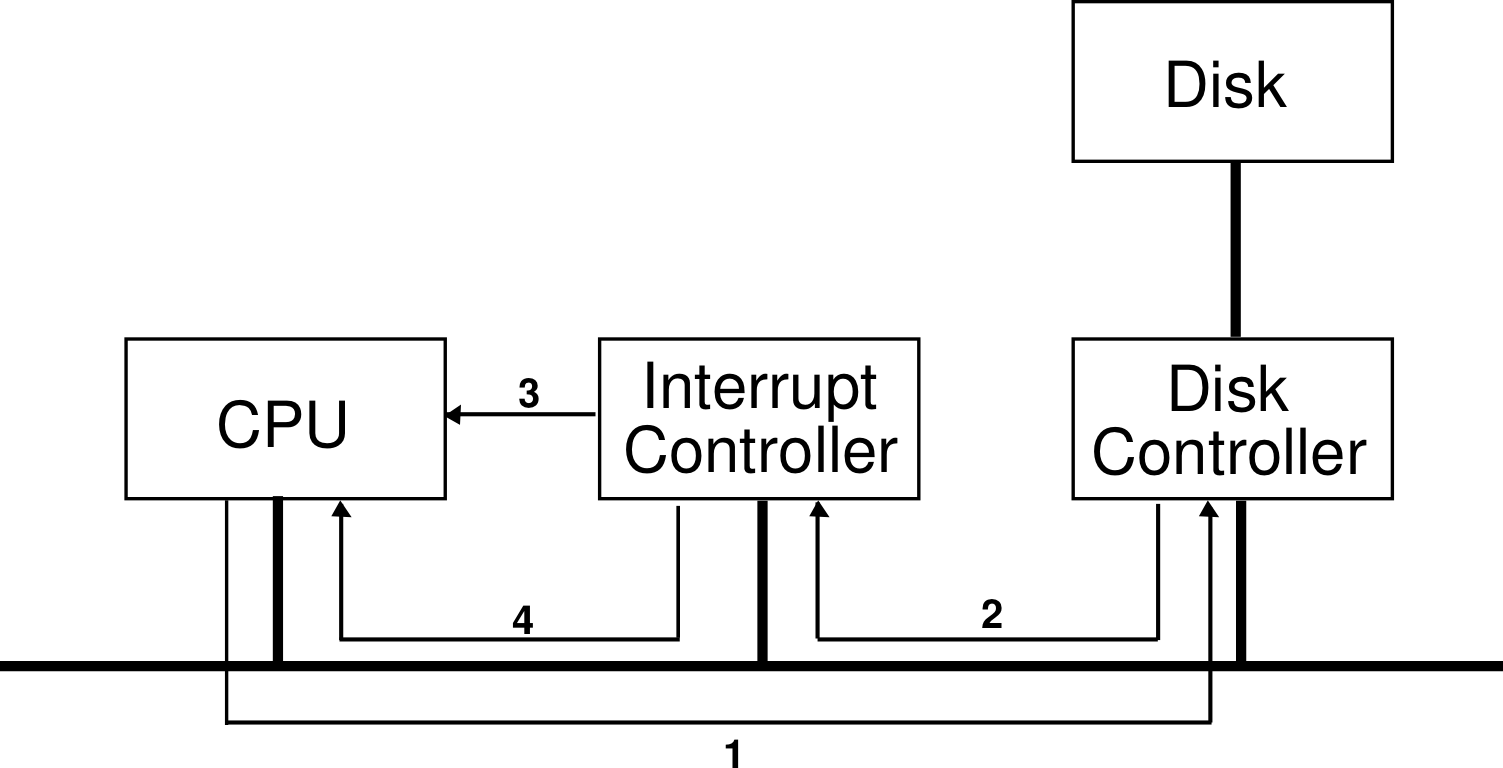
\includegraphics[width=80mm]{images/fig0202.png}
\end{center}
\caption{Lezen van een harde schijf}
\label{lezenhd}
\end{figure}

\begin{enumerate}
\item Schijfbesturingseenheid ontvangt een leesopdracht.
\item Wanneer de leesopdracht voltooid is stuurt de schijfbesturingseenheid een
interrupt request naar de \emph{interrupt controller}. Merk op dat de
processor tussen 1 en 2 \'e\'en of meer andere programma's heeft uitgevoerd.
\item De interrupt controller geeft de interrupt request door aan de processor. Wanneer
er een request met een hogere prioriteit wordt afgehandeld is het mogelijk dat
de schijf-interrupt hierop moet wachten. Dit is \'e\'en van de taken van de
interrupt controller.
\item Interrupt controller stuurt het volgnummer van de bron van de interrupt request
naar de processor, zodat die weet welk apparaat de request veroorzaakte.
\item De processor zoekt het adres op van de juiste Interrupt Handler in de
tabel met interrupt-vectoren.
\item De inhoud van de bevelenteller, alle registers en de processorstatus
worden op de stapel gezet.
\item Adres van Interrupt Handler wordt in bevelenteller geplaatst en de
processor wisselt naar kernel toestand.
\item Sprong naar het adres van de Interrupt Handler en de handler wordt
uitgevoerd. De code in de interrupt handler handelt het via de interrupt gedane
verzoek af. Deze handler is een onderdeel van het besturingssysteem, en een
gedeelte van de code zal uit de device driver van het onderbrekende apparaat
komen.
\item Als het werk erop zit herstelt de interrupt handler de bevelenteller,
registers en processortoestand en schakelt de processor terug in
gebruikerstoestand. Het programma dat in uitvoering was voor de interrupt wordt
verdergezet (want de bevelenteller wijst naar de volgende instructie in dat
programma).
\end{enumerate}

Het gevolg van een interrupt is dus dat een stuk code van het
besturingssysteem uitgevoerd wordt, dat specifiek bestemd is om de
opgetreden interrupt af te handelen, de Interrupt Handler. Deze zal
eerst nagaan wat de reden is van de interrupt en zal dan de gepaste
acties ondernemen.

Stappen 6 en 7 worden een \emph{context switch}\index{context switch}
genoemd. Een context switch wijzigt de toestand van de processor zodat
die een ander programma gaat uitvoeren, en bovendien zo dat de
toestand weer hersteld kan worden om verder te gaan met de uitvoering
van het programma dat in uitvoering was. De inhoud van de
bevelenteller, de registers en het statuswoord van de processor worden
weggeschreven op de stapel in het werkgeheugen. Deze gegevens worden
de context genoemd, vandaar de term context switch.

Merk op dat dit door de processor zelf afgehandeld wordt, en
niet door een stukje machine-code uit te voeren. Om dit stukje code
voor de context switch uit te voeren zou immers een context switch
nodig zijn...

\subsection{Snelheidswinst}

Nu dat we het concept van interrupts ge\"introduceerd hebben, kunnen we deze aanpak vergelijken met de standaard-aanpak waarbij er geen interrupts gebruikt worden. Figuur~\ref{fig:intsandnoints} toont de uitvoering van een programma zonder interrupts, en hetzelfde programma m\'et interrupts. Voor schema~\ref{fig:progflownoint} doorloopt het progamma de volgende stappen:

\begin{enumerate}
\item Het programma doet een berekening. Het wil uiteindelijk de resultaten wegschrijven naar de schijf, dus verstuurt het een aanvraag naar het besturingssysteem om de data weg te schrijven. Het programma zelf kan dit natuurlijk niet, aangezien het geen rechten heeft om rechtstreeks de hardware aan te spreken.
\item Het besturingssysteem evalueert de aanvraag en wanneer alles ok is stuurt het de data naar de schijf om deze weg te schrijven.
\item De schijf schrijft de data weg. De processor doet ondertussen niet veel nuttigs: hij blijft in een lus aan de schijf vragen of die al klaar is.
\item Uiteindelijk geeft de schijf aan dat het wegschrijven gedaan is, en sluit het besturingssysteem de schrijfopdracht af. Hierna gaat de processor terug naar de applicatie.
\item De applicatie gaat verder en sluit uiteindelijk af.
\end{enumerate}

Schema~\ref{fig:progflowwithint} toont de uitvoering van hetzelfde programma m\'et interrupts. Het doorloopt de volgende stappen:

\begin{enumerate}
\item Het programma doet een berekening. Het wil uiteindelijk de resultaten wegschrijven naar de schijf, dus verstuurt het een aanvraag naar het besturingssysteem om de data weg te schrijven.
\item Het besturingssysteem evalueert de aanvraag en wanneer alles ok is stuurt het de data naar de schijf om deze weg te schrijven.
\item De schijf schrijft de data weg. De processor gaat ondertussen terug naar de applicatie die verder kan rekenen terwijl de schijf data schrijft. De applicatie blijft actief totdat de schijf klaar is en een interrupt request stuurt.
\item De interrupt request wordt afgehandeld (d.i. een interrupt) en het besturingssysteem sluit de schrijfopdracht af. Hierna gaat de processor terug naar de applicatie.
\item De applicatie gaat verder en sluit uiteindelijk af.
\end{enumerate}

\begin{figure}
\centering
\begin{subfigure}{.5\textwidth}
  \centering
  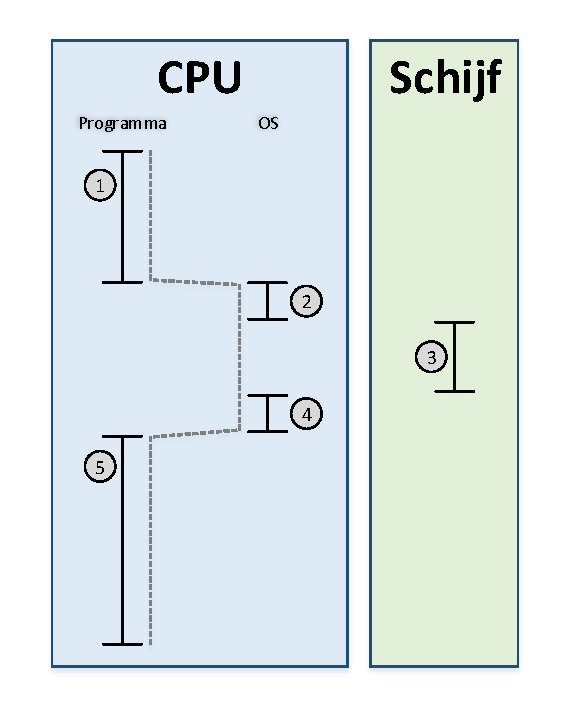
\includegraphics[width=.85\linewidth]{images/ProgramFlowNoInterrupts.pdf}
  \caption{Geen interrupts}
  \label{fig:progflownoint}
\end{subfigure}%
\begin{subfigure}{.5\textwidth}
  \centering
  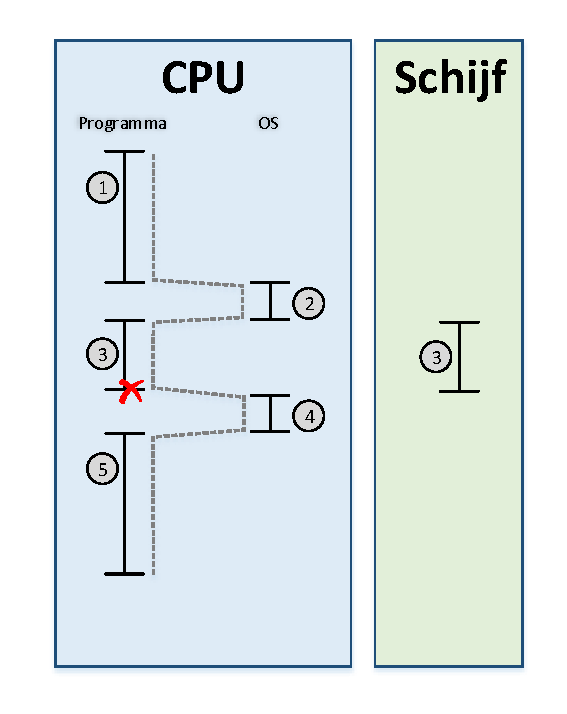
\includegraphics[width=.85\linewidth]{images/ProgramFlowWithInterrupts.pdf}
  \caption{Wel interrupts}
  \label{fig:progflowwithint}
\end{subfigure}
\caption{De uitvoering van een programma met en zonder interrupts.}
\label{fig:intsandnoints}
\end{figure}

Merk op dat het proces in schema~\ref{fig:progflowwithint} een aanzienlijke tijdswinst boekt, aangezien het tijdens het wegschrijven van data nog altijd kan blijven doorrekenen. Hier wordt het voordeel van interrupts dan ook duidelijk.

\subsection{Soorten interrupts}\label{sec:soorten}

Er zijn twee soorten interrupts: externe en interne.
\emph{Externe interrupts}\index{interrupt!extern} komen van hardware buiten de
processor. Enkele voorbeelden:

\begin{description}
\item[Klok interrupts] De interne klok van de computer signaleert hiermee aan de
processor dat een bepaalde tijdsperiode is verstreken.
\item[I/O interrupts] Wanneer via een randapparaat een I/O operatie is
uitgevoerd meldt de besturingseenheid die het randapparaat
bestuurt, op deze manier het einde van de I/O operatie (zoals in het voorbeeld
hierboven)
\item[Keyboard interrupts] Telkens wanneer een toets op het toetsenbordwordt
ingedrukt heeft dit een interrupt tot gevolg, die tot doel heeft het
overeenstemmende karakter te laten inlezen in een buffer zodat het programma
waarvoor de invoer bestemd is eraan
kan.
\item[Hardwarefouten] Wanneer de hardware een fout detecteert, zoals bijvoorbeeld
 een printer die een papierstoring detecteert, wordt er een interrupt request gegenereerd.
\end{description}

\emph{Interne interrupts}\index{interrupt!intern} worden veroorzaakt
door een gebeurtenis binnen de processor en kunnen nog eens worden
opgesplitst in twee groepen: uitzonderingen en software
interrupts.

\emph{Uitzonderingen} of \emph{exceptions} zijn het gevolg van een fout tijdens
de uitvoering van een instructie zoals het delen van een getal door
nul, het adresseren van een ongeldig adres in het geheugen of een
poging om in gebruikerstoestand een geprivilegieerde instructie uit te
voeren. Het besturingssysteem moet hier optreden, b.v. door het
overtredende programma af te sluiten en dit aan de gebruiker mee te
delen. Uitzonderingen die door het besturingssysteem kunnen hersteld worden noemen we we in
het Engels \emph{faults}. Zo valt een deling door nul onder de noemer 'faults', omdat het besturingssysteem die situatie kan corrigeren door bijvoorbeeld een exception in het desbetreffende programma te gooien. Andere uitzonderingen die niet hersteld kunnen worden, noemen we \emph{aborts}. Een abort kan je bijvoorbeeld krijgen wanneer er een deling door nul optreedt tijdens de uitvoering van een interruptroutine.

\emph{Traps}\index{trap} of \emph{software interrupts}\index{interrupt!software} zijn het gevolg van de uitvoering van speciaal
daarvoor voorziene instructies in een programma. Zo kunnen programma's
ook gebruik maken van de mogelijkheden van het interrupt mechanisme en
de hulp inroepen van het besturingssysteem. Als een programma b.v.
gegevens wil inlezen vanop de schijf zal het dit via een software
interrupt aan het besturingssysteem vragen. In Intel x86 assembler wordt de INT-instructie gebruikt om een
software interrupt aan te geven. Met deze instructie kan een getal
tussen 0 en 255 meegegeven worden.

Er is een subtiel verschil tussen de verschillende interrupt types: interne interrupts zijn
\emph{synchroon}\index{interrupt!synchroon}, terwijl externe interrupts \emph{asynchroon}\index{interrupt!asynchroon} zijn.

Bij synchrone interrupts gebeurt de afhandeling ``actief'' in die zin dat de code van de
actieve applicatie verwacht dat de interrupts afgehandeld worden en hier zelfs op steunt.

Asynchrone interrupts gebeuren niet op voorspelbare plaatsen in de applicatiecode. Ze zijn
``passief'' omdat de interrupt handlers gewoon wachten totdat de interrupt requests
uiteindelijk eens voorkomen. Ze zijn ook onafhankelijk van en ongerelateerd met de actieve applicatie.

Op de Intel x86 processor kunnen asynchrone interrupts gemaskeerd worden. Dat wil zeggen
dat er tijdelijk gekozen kan worden om die interrupts niet af te handelen. Synchrone
interrupts kunnen nooit gemaskeerd worden, maar aangezien deze enkel gegenereerd worden
door het actieve programma (en volledig afgehandeld worden eer het programma terug verder mag
gaan) gaat de ene synchrone interrupt normaal nooit een andere onderbreken. Soms kan dit
echter toch het geval zijn wanneer er een fout zit in het besturingssysteem. Vaak resulteert
dit in een crash van het besturingssysteem\footnote{Op Windows krijg je dan het alom bekende
\emph{blue screen of death}. Volgens Microsoft zijn ongeveer 25\% van de blue screens veroorzaakt
door een echte fout in de code van Windows, terwijl de overige 75\% veroorzaakt worden door drivers
van externe partijen.}.

\subsection{Interrupts identificeren}

Hoe wordt nu bepaald welke interrupt handler dient te worden
uitgevoerd wanneer een interrupt optreedt? Bij exceptions wordt de
interrupt door de processor zelf veroorzaakt, en kan de processor de
inhoud van de conditiecode in zijn toestandsbeschrijving
nagaan.

Wanneer een programma in uitvoering een trap-instructie doet
wordt de nodige informatie meegegeven om de juiste interrupt handler
te kiezen. In Intel x86 assembler is dit het getal dat je meegeeft aan de
INT-instructie. Natuurlijk hangt de betekenis van het getal af van het
gebruikte besturingssysteem.

In Intel x86 assembler programma's voor MS-DOS\index{besturingssysteem!MS-DOS} wordt vaak 'INT 21h'
opgeroepen. Deze software interrupt zorgt ervoor dat MS-DOS een
interrupt handler uitvoert. Deze specifieke interrupt handler is een
soort manusje-van-alles in MS-DOS, en je moet via het AH-register
aangeven wat je van de interrupt handler verwacht. Als er b.v. '4Ch'
in AH staat moet het besturingssysteem je programma be\"eindigen.

Bij hardware interrupts ligt de oorzaak buiten de processor, en
moeten we op zoek naar de bron van de onderbreking. Dat kan op 3
algemene manieren.

\begin{figure}
\begin{center}
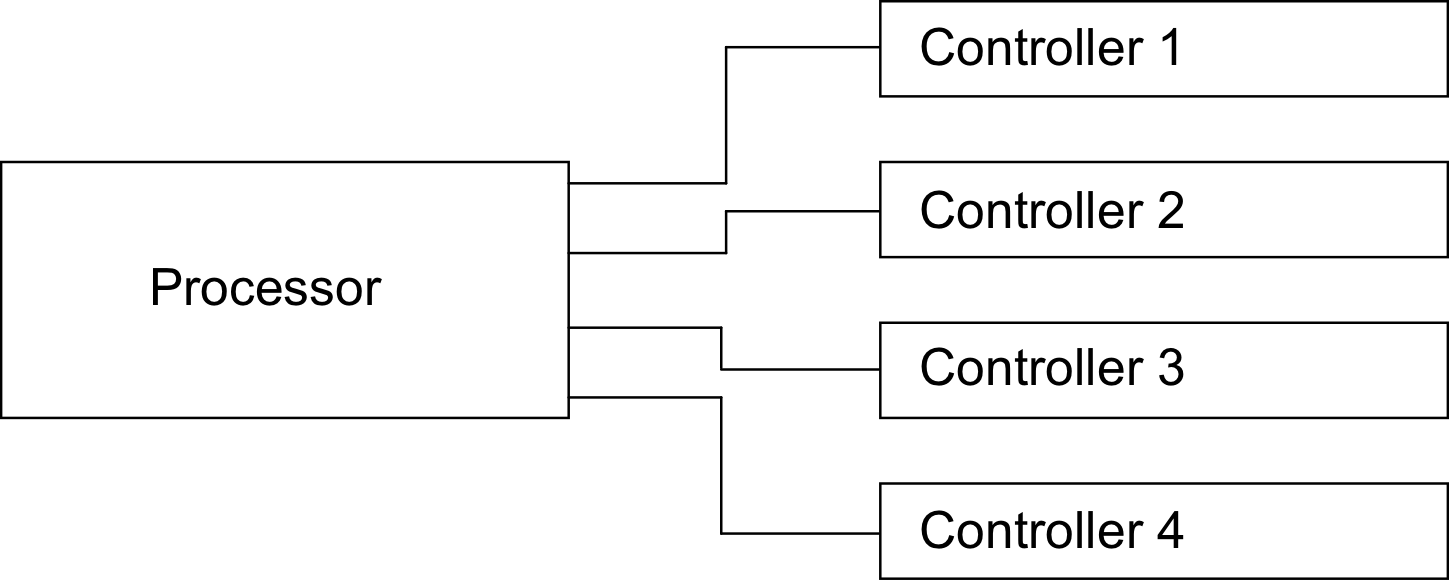
\includegraphics[width=80mm]{images/fig0203.png}
\end{center}
\caption{Controllers met eigen interruptlijnen}
\label{eigenlijn}
\end{figure}

Als iedere controller een eigen
\emph{interruptlijn}\index{interruptlijn} heeft, bepaalt de lijn waarop het
interruptsignaal verschijnt meteen welke handler moet worden
uitgevoerd (figuur \ref{eigenlijn}). Dit is een snelle en eenvoudige methode
maar legt
natuurlijk zware beperkingen op aan de configuratiemogelijkheden: het
aantal controllers is dan beperkt tot het aantal interruptlijnen in de
processor.

\begin{figure}
\begin{center}
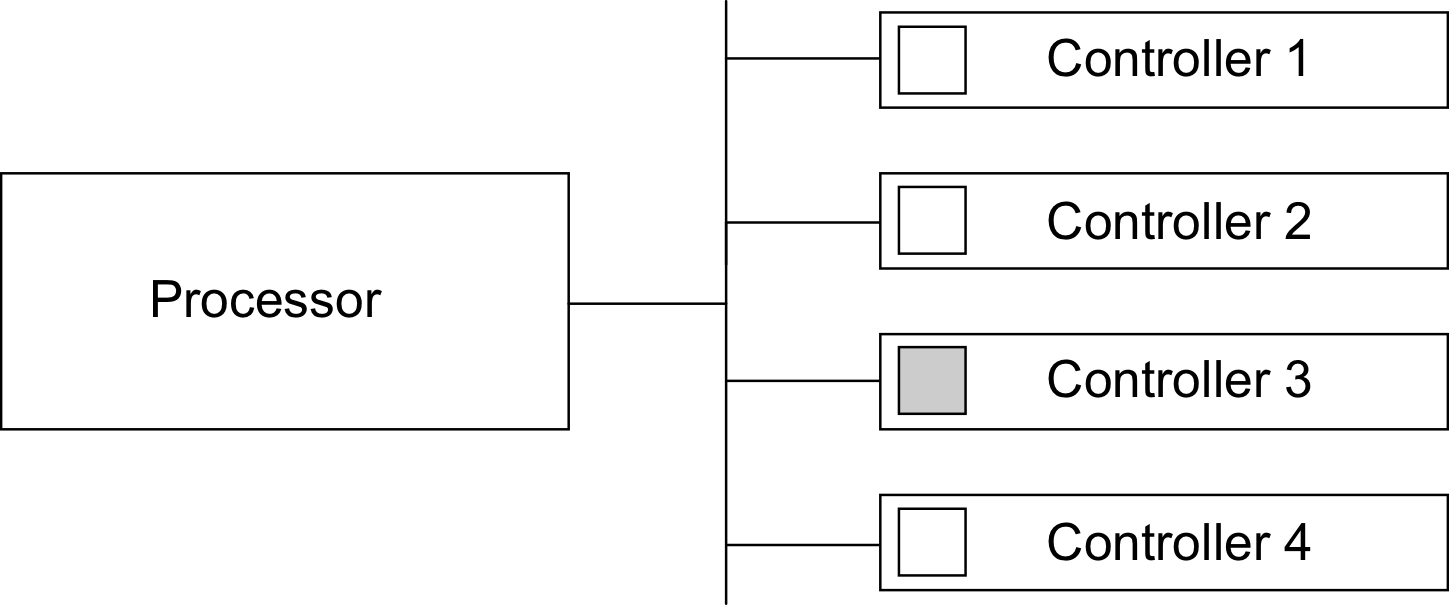
\includegraphics[width=80mm]{images/fig0204.png}
\end{center}
\caption{Software Polling}
\label{eenlijn}
\end{figure}

Als de controllers via \'e\'en lijn met de processor verbonden zijn
kan de controller d.m.v. een bit in \'e\'en van zijn registers aangeven of
hij een interrupt heeft gestuurd of niet. Na de context switch wordt
een routine uitgevoerd die aan \emph{software polling}
doet: achtereenvolgens elke controller controleren tot diegene wordt
gevonden die de interrupt veroorzaakte. Door het uitvoeren van deze
extra routine is dit een eerder trage methode.

\begin{figure}
\begin{center}
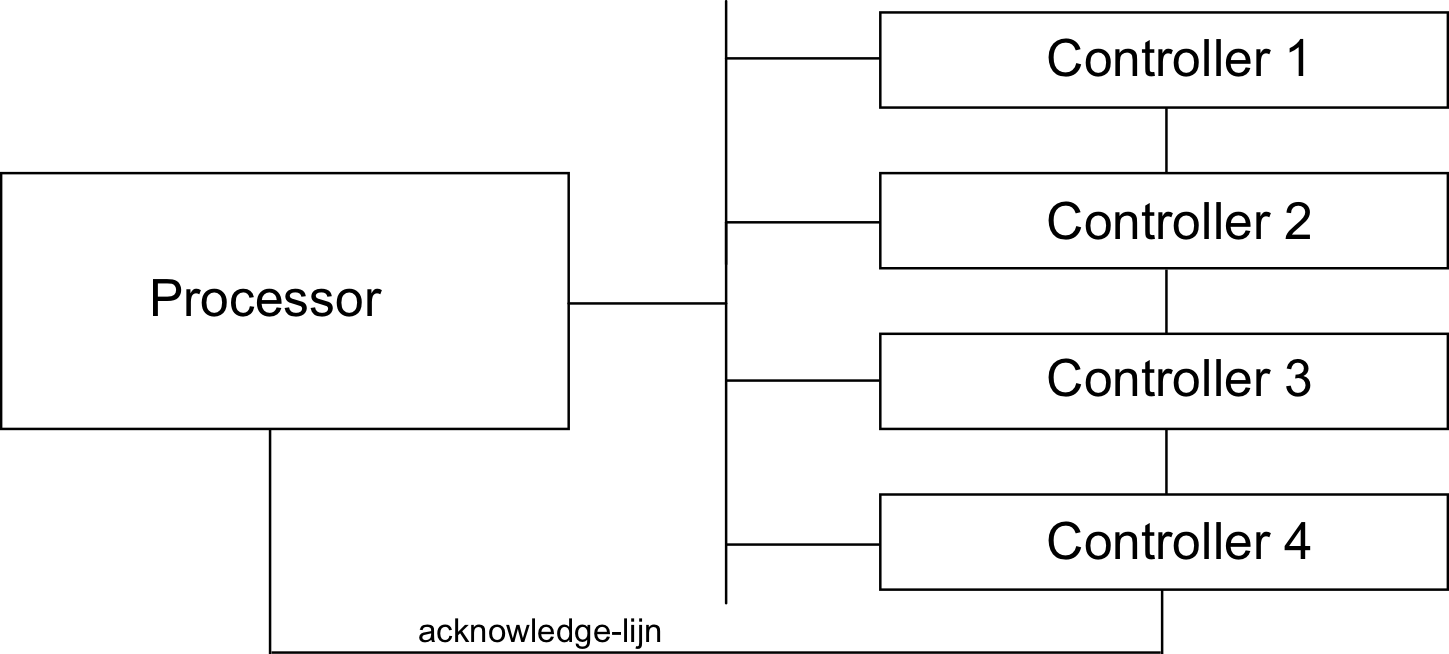
\includegraphics[width=80mm]{images/fig0205.png}
\end{center}
\caption{Daisy Chaining}
\label{daisy}
\end{figure}

Bij de derde manier zijn alle controllers via \'e\'en interruptlijn
en \'e\'en zogenaamde acknowledge-lijn met de processor verbonden. Zodra
een hardware interrupt optreedt zendt de processor via deze
acknowledge-lijn een signaal naar de eerste controller. Indien deze de
interrupt veroorzaakte stuurt hij een identificatiecode naar de
processor; in het andere geval geeft hij het signaal door naar de
volgende controller, die hierop op dezelfde manier reageert. Deze
werkwijze, \emph{daisy chaining}\footnote{In het algemeen is daisy chaining een
structuur waarin een apparaat A verbonden is met een apparaat B, B met C, C met
D, enz. Als A een signaal ontvangt stuurt hij het door naar B, eventueel na het
aanbrengen van een wijziging. De naam komt van het vormen van een slinger van
madeliefjes (Eng.: daisy) door een gaatje te maken in de stengel van een bloem
en er een andere bloem door te steken. Een ander voorbeeld van het gebruik van
een daisy chain structuur zijn SCSI-apparaten.}\index{daisy chaining} genoemd, is erg snel omdat ze
volledig via de hardware verloopt.

\subsection{Prioriteiten voor interrupts}

Het is soms belangrijk dat bepaalde interrupts voorrang krijgen
krijgen op minder belangrijke. De volgorde waarin interrupts worden
afgehandeld verdient dus ook aandacht.

Wanneer twee of meer interrupts tegelijk (of juister: tijdens
het uitvoeren van dezelfde instructie) optreden, moet er gekozen
worden welke interrupt eerst afgehandeld wordt. Beide interrupts zijn
hangende of pending. Vaak wordt gekeken naar de vereiste
\emph{interrupt latency}. Dit is de maximale tijd die
waarbinnen de interrrupt afhandeling moet begonnen zijn. De drivers
van audio- of video-hardware hebben een lage interrupt latency. Als
het te lang duurt vooraleer hun interrupts behandeld worden ontstaat
er kwaliteitsverlies.

Hoe we de prioriteit van interrupts kunnen bepalen hangt af van
de gebruikte identificatiemethode. Bij het gebruik van meerdere
interruptlijnen zal de processor zelf moeten beslissen aan welk
signaal hij eerst aandacht zal besteden. Bij software polling zal de
volgorde waarin de controllers worden nagekeken bepalend zijn voor de
prioriteit. Dit kan softwarematig worden ingesteld. Bij daisy chaining
is het de volgorde waarin de controllers worden aangesloten op de
acknowledge-lijn. Een duidelijk nadeel is hier dat een wijziging in de
prioriteit een ingreep in de hardware vereist.

Een tweede vraag die we ons moeten stellen is of we nieuwe
interrupts willen toelaten tijdens het afhandelen van een interrupt.
Vaak wordt een vlag voorzien waarmee alle interrupts tijdelijk
geblokkeerd worden. Andere systemen laten toe prioriteiten te
defini\"eren voor de interrupts, en tijdens de afhandeling van een
bepaalde interrupt worden alleen interrupts geaccepteerd met een
hogere prioriteit.

\section{System Calls}\label{systemcalls}

Interrupts vormen de schakel tussen het besturingssysteem en de
hardware. \emph{System calls} of
\emph{systeemaanroepen}\index{systeemaanroep (system call)} leggen een link tussen de
overige software en het besturingssysteem (zie figuur \ref{sysint}). Bij alle
activiteiten, uitgevoerd in gebruikerstoestand, is immers zeer frequent de
tussenkomst nodig van het besturingssysteem om operaties te kunnen uitvoeren die
alleen in kernel-toestand mogelijk zijn.

\subsection{Het uitvoeren van een system call}

Essentieel bij een system call is het overschakelen van de
processor naar kernel- toestand. Dit gebeurt altijd via een
trap-instructie (software-interrupt)\index{trap}, waardoor wordt vermeden dat na
het instellen van de kernel-toestand het gebruikersprogramma de
controle zou kunnen behouden. De trap-instructie zorgt er namelijk
voor dat de gepaste systeemroutine wordt gestart. Daartoe wordt als
operand voor de trap-instructie een code meegegeven. Extra informatie kan
eventueel in welbepaalde registers worden geplaatst.

Figuur~\ref{fig:systemcalls} toont hoe een programma zichzelf kan afsluiten door
de juiste software interrupt op te roepen. Op Intel x86 wordt de \texttt{int}-instructie
als trap-instructie gebruikt, terwijl op een ARM-processor de \texttt{swi}-instructie
gebruikt wordt. Afhankelijk van de operanden van deze instructie en de waardes in de registers
weet het besturingssysteem wat de applicatie wil doen.

\begin{figure}
  \centering
  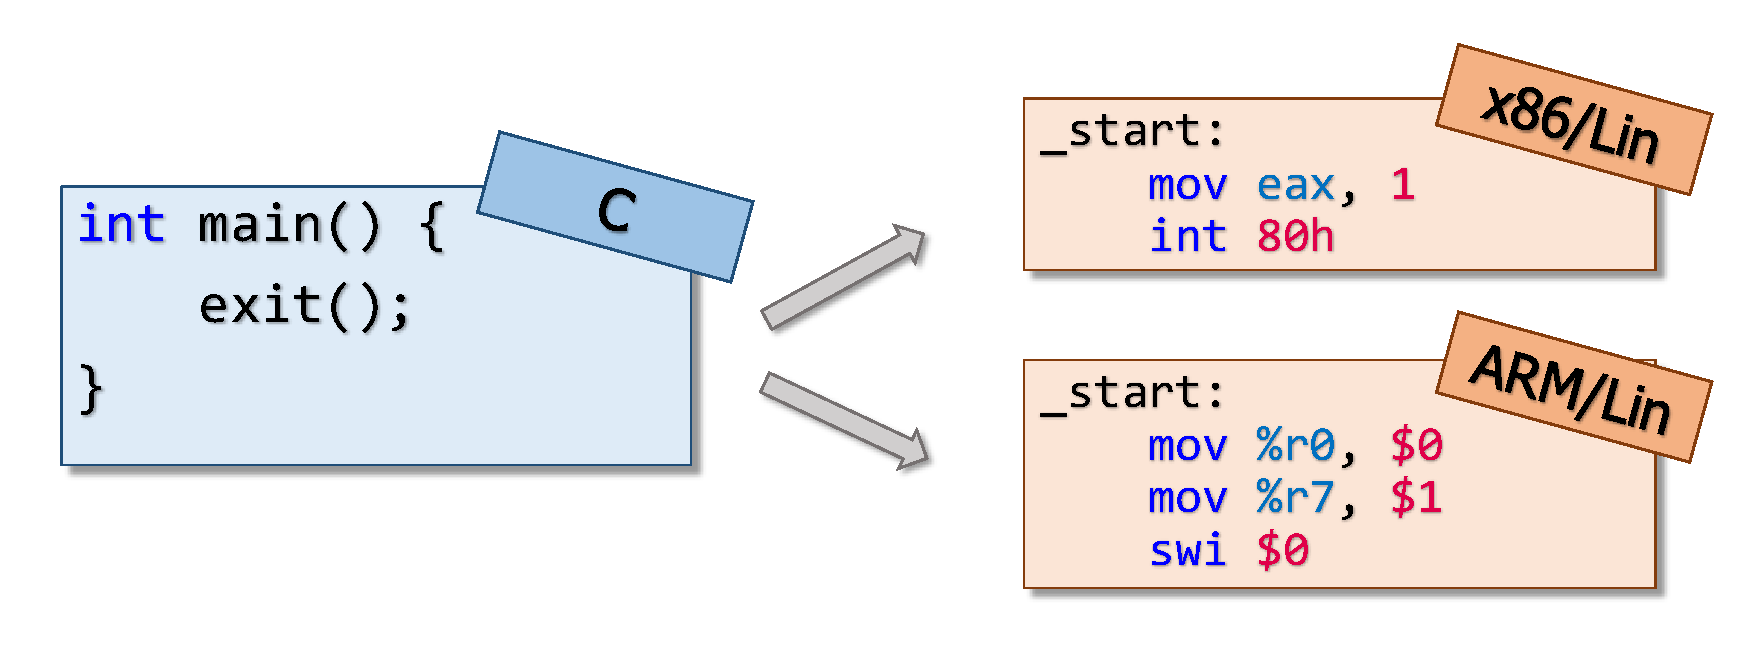
\includegraphics[scale=0.4]{images/IntInstructions.pdf}
  \caption{Het gebruik van traps om system calls uit te voeren.}\label{fig:systemcalls}
\end{figure}

Omdat de trap functioneert als een interrupt zal een interrupt
handler worden opgestart in kernel mode, die de meegegeven code zal
vertalen naar het beginadres van een specifieke systeemroutine. Aan de
hand van de code wordt tevens bepaald hoeveel bytes aan informatie als
parameters aan de systeemroutine moeten worden doorgegeven. Deze bytes
worden dan klaargezet, waarna de systeemroutine kan worden
opgeroepen.

Zodra de opdracht voltooid is wordt een eventueel resultaat (of
een foutmelding) op een afgesproken plaats gedeponeerd, waarna de
processor wordt teruggeschakeld naar user mode en tenslotte wordt
teruggekeerd naar het oproepend programma.

\subsection{Beschikbare system calls}

Dit is een overzicht van typische taken die toepassingssoftware
via system calls door het besturingssysteem kan laten
uitvoeren:

\begin{itemize}
\item Opstarten en be\"eindigen van programma's.
\item Laten wachten van een programma op een gebeurtenis.
\item Toekennen en vrijgeven van geheugen.
\item Bestandsbeheer.
  \begin{itemize}
  \item Cre\"eren en vernietigen van bestanden en directories.
  \item Openen en sluiten van bestanden.
  \item Lezen en schrijven in bestanden.
  \item Bepalen van de toegang tot bestanden.
  \end{itemize}
\item Besturing en beheer van randapparaten.
  \begin{itemize}
  \item Verwerven en afstaan van een randapparaat.
  \item Positioneren van een randapparaat.
  \item Lezen van en schrijven naar een randapparaat.
  \item Opnemen in of verwijderen uit de configuratie.
  \end{itemize}
\item Uitwisselen van informatie.
  \begin{itemize}
  \item Opvragen of wijzigen van informatie over:
    \begin{itemize}
    \item systeemconfiguratie
    \item uitgevoerde activiteiten
    \item processen
    \item bestanden en directories
    \item gebruikers
    \end{itemize}
  \end{itemize}
\item Communicatie
  \begin{itemize}
  \item Cre\"eren en opheffen van verbindingen (tussen systemen en processen)
  \item Zenden en ontvangen van boodschappen (tussen systemen, processen en
gebruikers)
  \end{itemize}
\end{itemize}

\subsection{Voorbeeld}

In het volgende voorbeeld simuleren we een oproep van de
read-system call in Linux\index{besturingssysteem!Linux}. Deze kan in de programmeertaal C opgeroepen
worden d.m.v. de functie \texttt{read(file\_desc, buffer, nbytes)}. Wanneer een
programma deze functie aanroept zal het volgende gebeuren:

\begin{enumerate}
\item Oproepend programma zet de waarden van de drie parameters op de stapel.
\item Read functie wordt aangeroepen (sprong naar code van read-functie).
\item Functie zet system call nummer in het juiste register en voert
TRAP-instructie uit (in Linux op een Intel x86 processor zou dit de instructies \texttt{mov eax, 3}
en \texttt{int 80h} opleveren; de 3 in eax geeft aan dat het om een lees-operatie gaat).
\item Besturingssysteem zoekt juiste routine op voor de system call.
\item BS start systeemroutine (sprong).
\item Systeemroutine zet resultaat op voorziene plaats, verlaat kernel mode en
geeft controle terug aan read-functie.
\item Read functie ontvangt de gegevens, zet ze op hun plaats en geeft controle
terug aan oproepend programma's.
\item Uitvoer oproepend programma gaat verder.
\end{enumerate}

Stappen 4 t/m 6 verlopen in kernel mode, de overige stappen worden in user mode
uitgevoerd.


\chapter{Bootproces}\label{bootproces}

\section{Opstarten}

Het opstartproces van een computer begint wanneer de voeding van
de computer ingeschakeld wordt. Bij het inschakelen controleert de
voeding zijn eigen spanningsniveaus. Wanneer de spanning stabiel is
tussen aanvaardbare waarden wordt een 'Power Good'\index{power good} signaal
gestuurd naar het moederbord. Het duurt typisch tussen 0,1 en 0,5
seconden voor de voeding stabiele stroom kan leveren.

Een halve seconde lijkt niet veel, maar de huidige processoren
voeren in die tijd miljoenen instructies uit. Om te vermijden dat het
systeem onder deze onstabiele omstandigheden zou beginnen opstarten
blijft het moederbord de processor continu resetten zolang er geen power
good signaal ontvangen wordt. Ook wanneer de computer al in gebruik is
verhindert dit mechanisme beschadiging of onzekere resultaten door
slechte stroomtoevoer. Bij problemen met de stroomvoorziening, zoals een
abnormale spanningswijziging op het stroomnet, zal het systeem zichzelf
herstarten omdat de processor weer tijdelijk het reset-signaal ontvangt
wanneer het power good signaal vanuit de voeding wegvalt.

Wanneer het reset-signaal wegvalt kan de processor beginnen
werken. De processor draait nu in kernel mode (d.i.: alle instructies
---ook de gepriviligeerde instructies--- zijn toegelaten) en gebruikt
uit compatibiliteitsoverwegingen \emph{real mode}\index{real mode}
als addresseringsmodus\footnote{Indien je niet meer weet wat \emph{real mode}
is, dan kan je dat best nog eens opzoeken in hoofdstuk 3 van de cursus
Computersystemen}. Maar welke code moet er uitgevoerd worden? Er zijn nog geen
instructies in het werkgeheugen geladen, dus de opstartcode moet elders
gevonden worden.

De oplossing voor dit probleem is om bepaalde adressen in de geheugenruimte niet
mappen op het werkgeheugen maar op iets anders. Dit noemt men \emph{memory mapped I/O}. Figuur~\ref{memorymapped}
toont de layout van de x86-geheugenruimte en welke stukken waarop gemapped worden.
Het rode stuk in de tekening is het stuk van de geheugenruimte waar de processor
de opstartcode verwacht. Concreet begint de processor instructies uit te voeren
vanaf adres 0xFFFFFFF0 (merk op dat dit adres binnen het rode stuk valt). Wanneer
de processor het geheugenadres 0xFFFFFFF0 opvraagt aan de geheugen controller, zal
die echter geen bytes vanuit het werkgeheugen halen, maar zal die de data halen uit
een ROM-chip op het moederbord. Deze ROM-chip bevat dan het opstartprogramma.

\begin{figure}
\centering
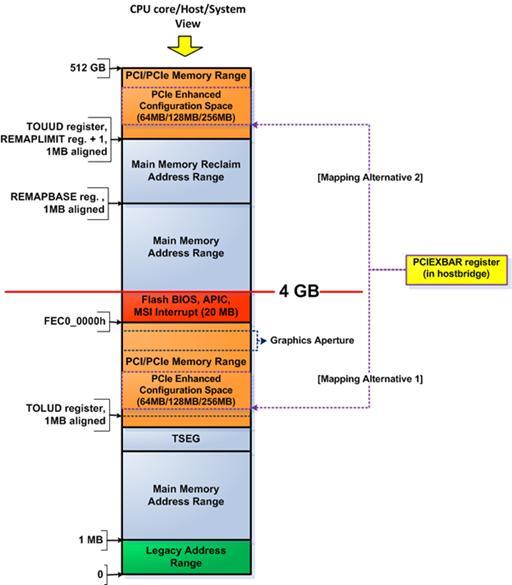
\includegraphics[scale=.75]{images/iomappedmemory.png}
\caption{De x86 memory layout. Leer deze grafiek alsjeblieft niet vanbuiten!}
\label{memorymapped}
\end{figure}

\section{Unified Extensible Firmware Interface}

Moderne systemen volgen de \emph{Unified Extensible Firmware Interface}-specificatie
(\emph{UEFI})\index{UEFI} om de computer verder op te starten. De UEFI-standaard zorgt voor afspraken omtrent een zogenaamde
\emph{pre-boot execution environment} die er voor zorgt dat de hardware ge\"initialiseerd
wordt en het besturingssysteem ingeladen wordt. Implementaties van deze standaard zijn in essentie een
mini-besturingssysteem die een aantal basisfunctionaliteiten aanbieden (zoals bijvoorbeeld
het starten van het hoofdbesturingssysteem).

De belangrijkste eigenschappen die de UEFI-standaard voorziet, zijn:

\begin{itemize}
\item \textbf{Ondersteuning voor grote schijven} De voorganger van UEFI ---{} het Basic Input/Output System (BIOS)\index{basic input/output system} ---{} bood maar ondersteuning voor harde schijven tot 2TB. De UEFI-standaard verhoogt deze limiet tot 8ZB (d.i. 8 miljard terabyte).
\item \textbf{CPU-onafhankelijke architectuur} De UEFI-specificatie is zo opgesteld dat de services die worden aangeboden niet processor-specifiek zijn. Er zijn dan ook UEFI-implementaties voor de x86-, x86-64-, ARM-, ARM64-, en Itanium-processoren.
\item \textbf{CPU-onafhankelijke stuurprogramma's} EFI Byte Code (EBC) is een processor-onafhankelijke machinetaal die een beetje vergelijkbaar is met Java bytecode\footnote{https://en.wikipedia.org/wiki/Java\_bytecode} of Common Intermediate Language\footnote{https://en.wikipedia.org/wiki/Common\_Intermediate\_Language}. Een UEFI-implementatie kan dan een vertolker bevatten om die EBC uit te voeren. Zo moet een auteur van een stuurprogramma slechts \'e\'en versie van het stuurprogramma schrijven (in EBC), dat dan op alle processorarchitecturen waar UEFI op ondersteund wordt kan gebruikt worden.\footnote{In praktijk gaan hardwareontwerpers echter nog vaak processor-specifieke drivers voorzien omdat die vaak een stuk sneller zijn dan de EBC-varianten.}
\item \textbf{Modulair ontwerp} De UEFI-standaard voorziet een aantal mogelijke diensten die kunnen aangeboden worden, maar niet alle diensten \emph{moeten} aangeboden worden.
\item \textbf{Flexibele pre-OS omgeving} Hardwareverkopers krijgen de vrijheid om te kiezen hoe de layout van de pre-OS-omgeving eruit ziet en welke features ze willen ondersteunen. Verder kunnen gebruikers ook nog UEFI-applicaties installeren die dan uitgevoerd worden voordat het besturingssysteem opgestart is. Voorbeelden van zulke applicaties zijn bijvoorbeeld \emph{boot loaders} die dienen om de gebruiker te laten kiezen tussen verschillende besturingssystemen die ge\"installeerd zijn.
\item \textbf{Backward en forward compatibiliteit} UEFI voorziet een compatibiliteits-module om achterwaarts compatibel te zijn met besturingssystemen die geschreven zijn voor de BIOS-voorganger. Verder proberen de auteurs van UEFI ook voorwaarts compatibel te zijn, zodat nieuwe technologie\"en naadloos kunnen gebruikt worden op reeds bestaande UEFI-systemen.
\end{itemize}

UEFI voorziet \emph{boot services} en \emph{runtime services}. Boot services zijn enkel beschikbaar voordat het besturingssysteem opgestart is. Zo zijn er services om uitvoer op het scherm te tonen, communicatie met hardware te verzorgen, enz. De runtime services blijven beschikbaar, ook wanneer het besturingssysteem operationeel is. Zo kan het besturingssysteem bijvoorbeeld de datum en de tijd opvragen, of kan het kleine stukjes data opslaan in de chip waar de UEFI-implementatie in staat.\footnote{Dit is ook de reden waarom je bij het vervangen van een harde schijf je Windows 10 productsleutel niet opnieuw moet ingeven; de Windows 10-setup gaat automatisch je productsleutel opslaan in de UEFI-chip, zodat je die later niet meer opnieuw moet ingeven.}

\begin{figure}
\centering
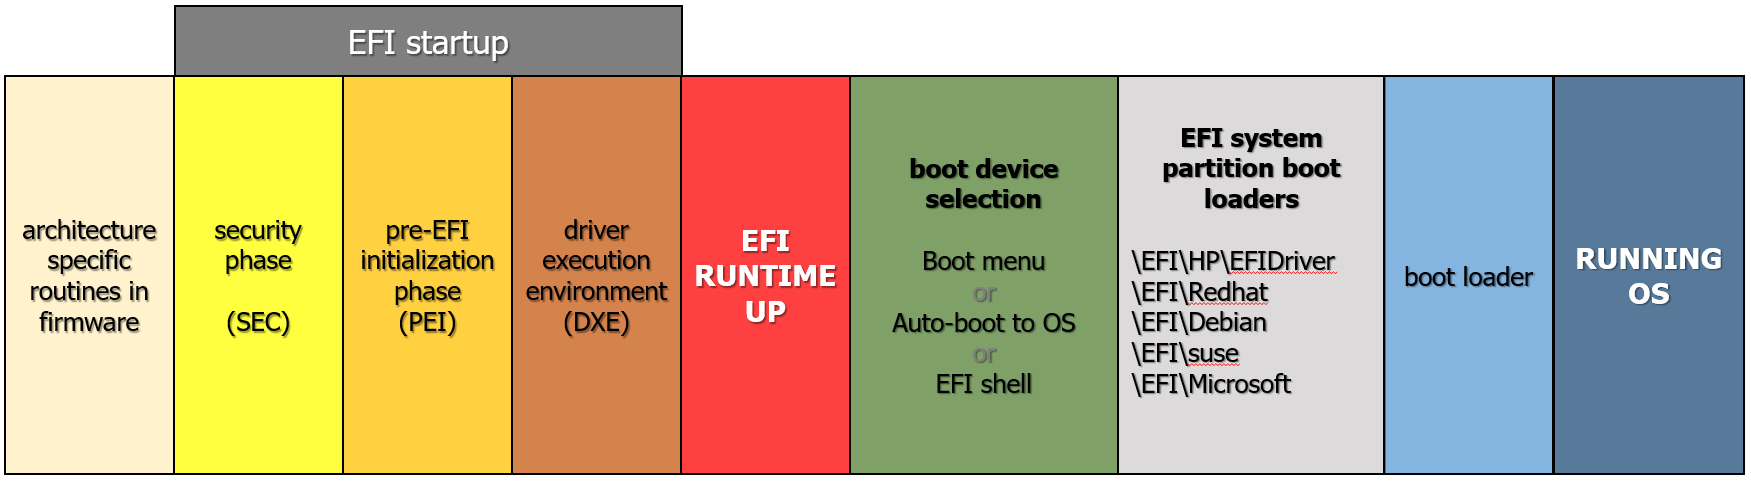
\includegraphics[scale=.25]{images/uefisartup.png}
\caption{Het UEFI boot-proces}
\label{uefiboot}
\end{figure}

De UEFI-specificatie voorziet een aantal fases tijdens het opstarten, zoals weergegeven in figuur~\ref{uefiboot}.
De \emph{security phase} (SEC) controleert dat de code van de UEFI-implementatie correct is en niet aangepast
werd door een potenti\"ele aanvaller. Als een hacker de opstartcode zou kunnen aanpassen, dan zou dat vanzelfsprekend
een zeer groot beveiligingsprobleem zijn. Het doel van de \emph{pre-EFI initialization phase} (PEI) is het opzetten van
een stuk werkgeheugen die de opstartcode kan gebruiken om bijvoorbeeld de UEFI-applicaties in te laden. De \emph{driver
execution phase} (DXE) doet dan het meeste werk wat betreft de initialisatie van het systeem. Hier worden de boot- en
runtime service opgezet, worden hardware-componenten ge\"initialiseerd (harde schijf, netwerk, ...), en worden er abstracties
gecre\"erd voor onder andere de verschillende boot devices.

De UEFI-specificatie is nogal vaag over wat er precies moet gebeuren wanneer de machine opgestart wordt. Typisch zullen
UEFI-implementaties tijdens de DXE-fase beginnen met het oplijsten van alle beschikbare stukken hardware en controleren
of die correct werken. Het geheel van deze tests wordt \emph{Power-On Self Test}\index{power-on self test} genoemd, of
kortweg \emph{POST}. Op sommige systemen kan je kiezen om deze POST aan te passen of grotendeels over te slaan. Het
voordeel is dan dat je computer sneller opstart, maar je zal een aantal opties (zoals het opstarten vanaf een USB stick)
niet meer kunnen gebruiken.

Als de initialisatie succesvol voltooid is zal de UEFI-code beginnen met
het laden van het besturingssysteem. Dit staat typisch op een
secundair opslagapparaat. Wanneer een computersysteem meerdere van
dergelijke opslagapparaten bevat moet de gebruiker aangeven vanop
welk apparaat een besturingssysteem geladen moet worden. Het
besturingssysteem kan op een harde schijf staan, maar het zou ook op
een CD-ROM, diskette of USB-opslagapparaat. In welke volgorde op alle
aanwezige apparaten naar een besturingssysteem gezocht moet worden
staat in de zogenaamde \emph{opstartvolgorde} of
\emph{boot sequence}\index{boot sequence}. De gebruiker kan deze opstartvolgorde naar eigen keuze aanpassen.

\section{Schijven en partities}

Als in de opstartvolgorde verwezen wordt naar een harde schijf
is de vraag weer hoe we het besturingssysteem terugvinden. De schijf kan in verschillende stukken
opgedeeld zijn (zogenaamde \emph{partities})\index{partitie}, en op eender welke partitie kan het besturingssysteem staan.
Het is aan de gebruiker om via de UEFI-gebruikersinterface de juiste partitie te kiezen.

Het opsplitsen van een schijf in verschillende stukken heeft praktisch nut:
\begin{itemize}
\item Er kan een partitie worden gemaakt voor de bestanden van het besturingssysteem, die enkel bestaat uit de snelste sporen van de schijf.\footnote{\textbf{vraag:} \emph{Welke sporen op de harde schijf zijn de snelste? Denk aan de `zone bit recording'-technologie die in Computersystemen besproken is.}}
\item Het systeem is iets robuuster: je kan makkelijker de beveiliging per partitie instellen, als een programma vanwege een bug de schijf helemaal vult dan heb je daar maar last van op \'e\'en partitie, ...
\item Verschillende partities kunnen verschillende besturingssystemen bevatten (dit noemt men een zogenaamde \emph{multiboot}-opstelling)\index{multiboot}.
\item Zorgt voor een duidelijk scheiding tussen bijvoorbeeld het systeem en databestanden.
\item ...
\end{itemize}

Indien de gebruiker op meerdere partities een besturingssysteem ge\"installeerd heeft, dan kan er een
\emph{boot menu}\index{boot menu} gebruikt worden. Het boot menu toont tijdens het opstartproces een lijst van alle
ge\"installeerde besturingssystemen en laat de gebruiker kiezen welke hij wil opstarten. Figuur~\ref{fig:bootloaders}
toont twee voorbeelden van boot menus.

\begin{figure}
\centering
\begin{subfigure}{.5\textwidth}
  \centering
  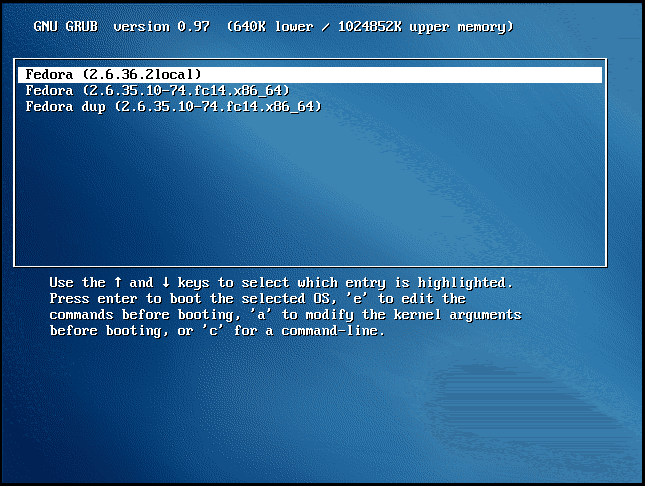
\includegraphics[width=.95\linewidth]{images/grubbl.png}
  \caption{De GRUB boot manager}
  \label{fig:grubnl}
\end{subfigure}%
\begin{subfigure}{.5\textwidth}
  \centering
  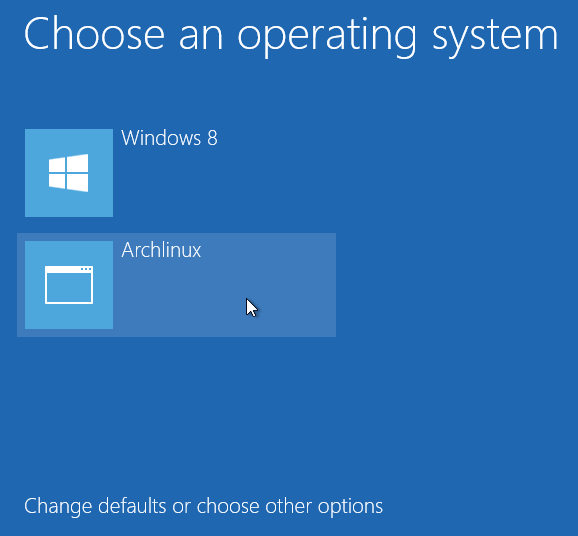
\includegraphics[width=.95\linewidth]{images/wbl.png}
  \caption{De Windows boot manager}
  \label{fig:wbl}
\end{subfigure}
\caption{Twee verschillende UEFI boot managers}
\label{fig:bootloaders}
\end{figure}

Informatie over de partities wordt op de schijf zelf opgeslagen op een gestandardiseerde manier. UEFI ondersteunt de oudere \emph{master boot record}-manier\index{master boot record} (MBR) om partitie-informatie op te slaan, maar deze manier biedt maar ondersteuning voor schijven tot 2TB. Bij voorkeur wordt dan ook het nieuwere \emph{GUID partition table}-systeem\index{GUID partition table} (GPT) gebruikt. GPT biedt ondersteuning voor schijven tot 8ZB (d.i. 8 miljard TB).

Figuur~\ref{fig:gpt-layout} toont de layout van een GPT-schijf. Het eerste blok bevat een \emph{protective master boot record}\index{protective master boot record} voor compatibiliteitsdoeleinden met oudere systemen die geen GPT ondersteunen. Deze protective master boot record is grotendeels leeg, en bevat slechts informatie over \'e\'en partitie die de hele schijf beslaat (of voor schijven groter dan 2TB: zo veel plaats beslaat als mogelijk). Het partitietype staat op \byte{EE} wat betekent dat de partitie in feite een GPT-partitie is. Tools die GPT niet ondersteunen zullen dit partitietype niet herkennen, en zouden normaal gezien de partitie (en dus de schijf) met rust laten.

\begin{figure}
\centering
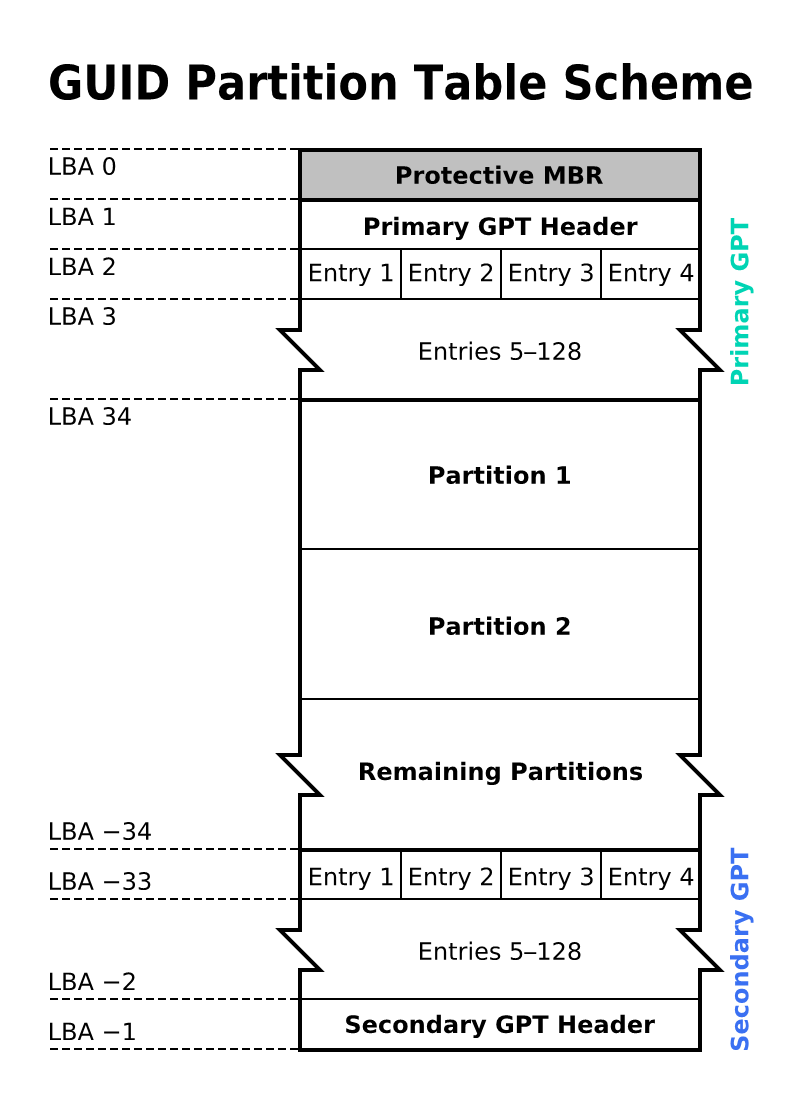
\includegraphics[scale=1]{images/gpt-layout.png}
\caption{De layout van een GPT-schijf}\label{fig:gpt-layout}
\end{figure}

Na de protective MBR staat de primaire GPT header. Deze header bevat informatie over de schijf (grootte, beschikbare sectors, ), een uniek identificatienummer van de schijf, en een wijzer naar een backup-kopie van de header. Deze backup-kopie staat helemaal aan het eind van de schijf en bevat exact dezelfde informatie. Als de primaire header beschadigd raakt, dan kan de backupkopie gebruikt worden om alsnog de partitie-informatie uit te lezen.

Na de primaire GPT header volgt een lijst van \emph{partition entries}.\index{partition entry} Elk van deze entries kan informatie bevatten over \'e\'en partitie. Zo bevat een entry onder andere informatie over het partitietype, een uniek identificatienummer, de start- en eindsector, en de attributen van de partitie (alleen-lezen, verborgen, ...). Ook van de lijst van partition entries wordt een backup op het einde van de schijf bijgehouden.

\begin{figure}
\begin{center}
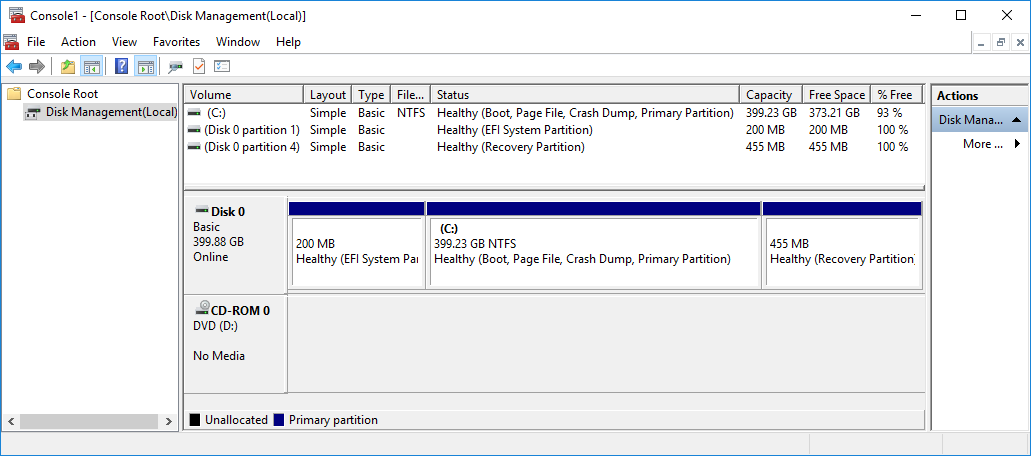
\includegraphics[width=125mm]{images/diskmgr.png}
\end{center}
\caption{Drie GPT-partities}
\label{efisyspart}
\end{figure}

Figuur~\ref{efisyspart} toont een harde schijf met drie partities. De eerste partitie
is van het type \emph{EFI System Partition} en bevat o.a. alle programma's die in de
UEFI-implementatie uitgevoerd kunnen worden. De tweede partitie bevat in dit geval het
besturingssysteem en is gemarkeerd als \emph{bootable}. Als laatste is er nog een partitie
gedefini\"eerd voor recovery-doeleinden.

Wanneer de UEFI-omgeving opgestart is (d.w.z. de DXE-fase klaar is, zie figuur~\ref{uefiboot}), moet er een
boot device gekozen worden. Hiervoor wordt gebruik gemaakt van een \emph{boot menu}\index{boot menu}-applicatie
die aan de gebruiker vraagt welk besturingssysteem hij wil opstarten. Indien er maar
een besturingssysteem op de computer ge\"installeerd is, is de vraag natuurlijk overbodig
en wordt dit OS direct opgestart. Deze applicatie kan meegeleverd worden door de UEFI-fabrikant, maar kan
ook op de EFI System Partition worden ge\"installeerd bij de installatie van een besturingssysteem op je computer.
Wanneer je bijvoorbeeld Windows installeert, zal de Windows-installatie Microsoft's
boot menu op de EFI System Partition zetten waarmee Windows (en eventueel andere besturingssystemen)
opgestart kan worden.

Eenmaal de gebruiker een besturingssysteem geselecteerd heeft, wordt er een \emph{partition boot loader}\index{partition boot loader}-applicatie opgestart die het besturingssysteem op de geselecteerde partitie zal inladen. Afhankelijk van de gekozen
partitie zal de juiste partition boot loader geselecteerd worden. De taak van de partition boot loader is om op de partitie
de code te zoeken die het besturingssysteem verder gaat inladen. Kwestie van de zaken wat gecompliceerd te maken, noemen ze deze code
de \emph{boot loader}\index{boot loader}. Zorg dus dat je de termen \emph{boot loader} en \emph{partition boot loader} niet door elkaar
haalt.

De boot loader staat op de partitie van het besturingssysteem en is dus geen deel van de UEFI-implementatie. Als de partitie
bijvoorbeeld een (recente) Windows-installatie bevat, dan zal de boot loader in de eerste sector van de partitie staan\footnote{Indien de eerste sector van de schijf een boot loader bevat, wordt deze sector ook de \emph{partition boot block} of het \emph{partition boot record} genoemd.\index{boot sector}} en het
programma \emph{BOOTMGR} opstarten. BOOTMGR is dan de laatste schakel in het bootproces. Dit programma gaat de feitelijke code van Windows inladen en opstarten. Figuur~\ref{bootsteps} geeft een overzicht van de verschillende stappen in het opstartproces.

\begin{figure}
\begin{center}
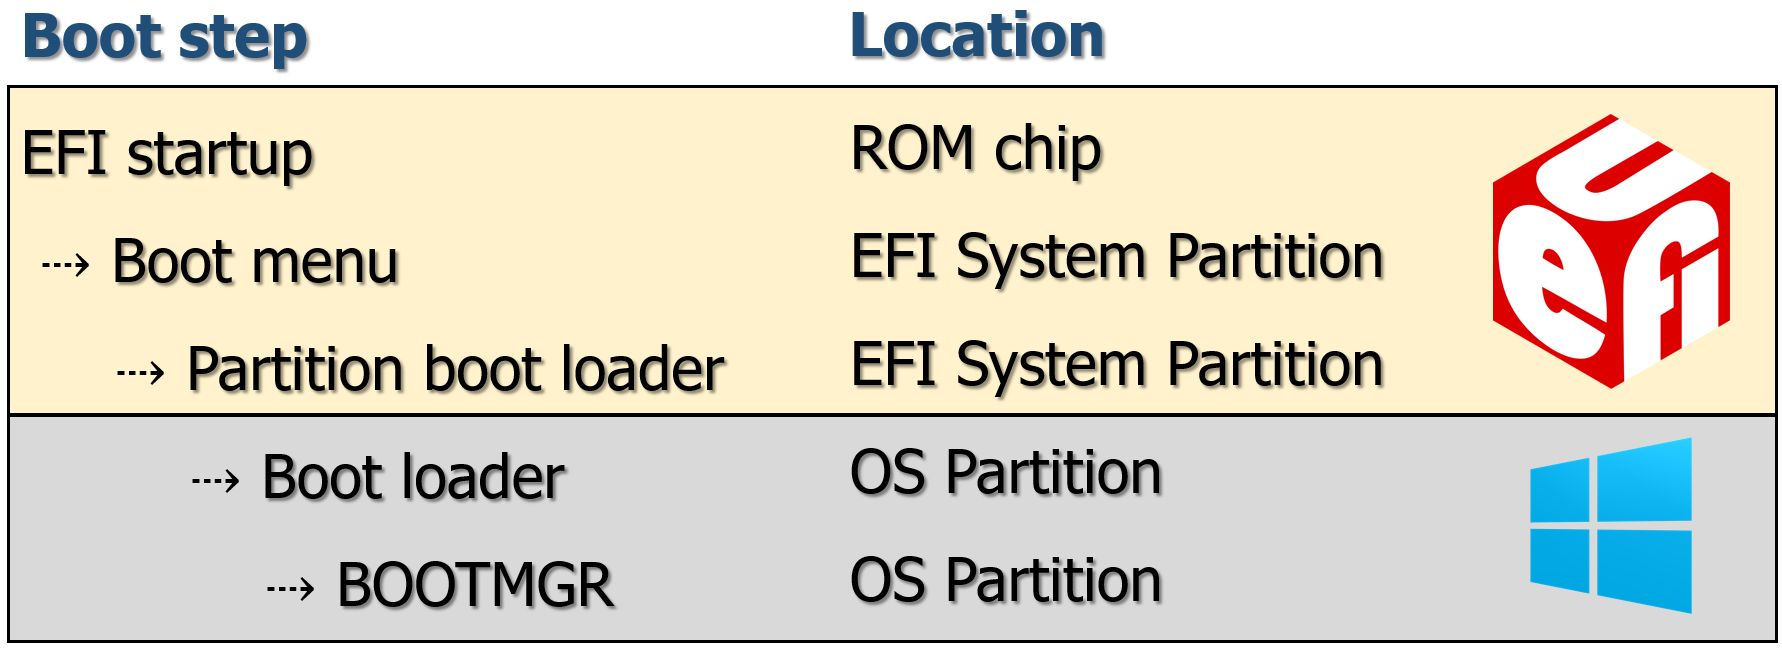
\includegraphics[width=125mm]{images/startupsteps.png}
\end{center}
\caption{De stappen in het opstartproces}
\label{bootsteps}
\end{figure}

\chapter{Bestandssystemen}

Een computerprogramma is een verzameling instructies die toegepast
wordt op invoergegevens. Het resultaat zijn opnieuw gegevens: de uitvoer.
De gebruiker van een computersysteem wil deze gegevens vaak bewaren.
Computersystemen hebben er naast gegevensverwerking een taak bijgekregen:
gegevensopslag.

Het onderdeel van het besturingssysteem dat instaat voor de
permanente opslag van gegevens is het
\emph{bestandssysteem}.\index{bestandssysteem} De term bestandssysteem wordt ook
soms gebruikt voor de in het systeem opgeslagen gegevens zelf. De
doelstellingen van het bestandssysteem zijn opnieuw samen te vatten als
gebruiksgemak en effici\"entie.

De gebruiker verwacht van het besturingssysteem dat het persistente
gegevensopslag aanbiedt. Het moet eenvoudig zijn om de gegevens te
organiseren en logisch te ordenen. De gegevenstoegang moet zo snel
mogelijk gaan, en er moet gestreefd worden naar een zo goed mogelijk
gebruik van de beschikbare capaciteit. Een bijkomende vereiste voor veel
systemen is het beveiligen van de gegevens, zodat b.v. verschillende
gebruikers van het systeem geen toegang hebben tot mekaars
gegevens.

\section{Fysische vs Logische gegevensordening}

\subsection{Fysische ordening: Sectoren}

Een \emph{sector}\index{sector} is de kleinste adresseerbare
eenheid voor gegevensopslag op een harde schijf. Een veelvoorkomende
waarde voor de sectorgrootte van een schijf is 512 bytes. Wanneer we
beschikken over een harde schijf, kunnen we dus blokjes gegevens van
512 bytes wegschrijven op een bepaald adres, en ze later terug vanop
dat adres inlezen. Hoe de gegevens over (de sectoren van) de harde
schijf verdeeld zijn noemen we de \emph{fysische
ordening} van de gegevens.

\subsection{Logische ordening: Bestanden}

De harde schijf biedt ons dus persistente gegevensopslag, maar
van gebruiksvriendelijkheid is weinig sprake. Een gebruiker wil een
\emph{logische gegevensordening}, die er b.v. voor zorgt
dat gegevens makkelijk terug te vinden zijn. In de logische ordening
wordt als basiselement meestal het bestand gebruikt. Een
\emph{bestand}\index{bestand} is een persistent opgeslagen logische
verzameling gerelateerde gegevens.

De taak van het bestandssysteem kan omschreven worden als het
aanbieden van een gebruiksvriendelijke en logisch geordende toegang
tot de fysische opslagmedia. Het bestandssysteem vertaalt het logische
beeld van de gebruiker en de bijhorende operaties in de fysische
schijftoegangen. De gebruiker of de programma's die hij uitvoert
moeten afgeschermd worden van de complexiteit en de benodigde
boekhouding. Zo wordt een bestand altijd voorgesteld als een
aaneengesloten reeks gegevens, zelfs als dat in de fysische ordening
niet zo is. Het opzetten van de nodige gegevensstructuren voor de
fysische ordening van een bestandssysteem op een partitie noemt men
\emph{formatteren}.\index{formatteren}

\section{Bestanden}

Een bestand is een verzameling gerelateerde gegevens, die door een
gebruiker of een applicatie op een bepaalde manier ge\"interpreteerd
worden.

Opdat de gebruiker de bestanden gemakkelijk kan aanspreken krijgen
ze een naam, en opdat het bestandssysteem de gegevens kan terugvinden
moeten de adressen van de gebruikte sectoren bijgehouden worden. Het
bestandssysteem verzamelt alle gegevens over een bestand in de
\emph{bestandsbeschrijving} of \emph{file
descriptor}.\index{file descriptor}

De \emph{bestandsnaam} verhoogt het gebruiksgemak
doordat de gebruiker zijn bestanden eenvoudig kan identificeren. Voor de
goede werking van het bestandssysteem is een betekenisvolle naam niet
noodzakelijk.

In ieder bestandssysteem zijn er beperkingen aan de maximale
lengte en de toegelaten karakters voor de naam. De lengte van de naam
kan beperkt zijn door de beschikbare ruimte in de bestandsbeschrijving.
Welke karakters toegelaten zijn hangt af van de gebruikte codering (b.v.
ASCII of Unicode) en het vermijden van tekens die in het systeem een
speciale betekenis hebben. Zo worden vaak de '\textbackslash' of '/' gebruikt als
scheidingsteken waardoor ze niet gebruikt kunnen worden in een
bestandsnaam. Ook de hoofdlettergevoeligheid van het bestandssysteem
be\"invloedt de mogelijke bestandsnamen. Sommige systemen leggen een vaste
structuur op aan de naam. Een voorbeeld hiervan is de '8+3' structuur in
MS-DOS. De eigenlijke naam kan 8 tekens lang zijn, en wordt aangevuld
met een extensie van 3 tekens, die aangeeft welk soort gegevens het
bestand bevat.

Naast de bestandsnaam worden in de bestandsbeschrijving allerlei
andere \emph{bestandskenmerken}\index{bestandskenmerken} bijgehouden. Deze zijn
voor ieder bestandssysteem anders, maar meestal vindt men minstens de
grootte van het bestand en de tijdstippen waarop het bestand aangemaakt
en/of voor het laatst gewijzigd werd. In een besturingssysteem met
meerdere gebruikers zal ook de eigenaar van het bestand worden vermeld en
op welke manier de toegang tot het bestand wordt geregeld. Verder kan de
aard van de inhoud, de interne structuur van het bestand of een
verplichte periode van bewaring opgeslagen zijn.

Aangezien het bestandssysteem een opgegeven bestandsnaam moet
vertalen naar de plaats waar de gegevens van het bestand zich bevinden
op het extern geheugenmedium moet er ook een
\emph{plaatsaanduiding} bijgehouden worden. De manier
waarop de plaatsaanduiding wordt opgenomen in de file descriptor hangt
af van de manier waarop de fysische gegevens bewaard worden.

Om de fysische gegevenstoegang te organiseren kunnen ook extra
gegevens over de toestand van het bestand nodig zijn. Zo kan het
belanrijk zijn om te weten of het bestand in gebruik is, en of er een
kopie bestaat in het werkgeheugen of elders op de schijf.

\section{Directories}

Een computersysteem bevat tegenwoordig gemakkelijk enkele
tienduizenden bestanden. Om een overzicht mogelijk te maken in de
massale hoeveelheden aanwezige informatie is het noodzakelijk dat, net
als in een bibiotheek, een catalogus beschikbaar is. De gebruiker krijgt
vaak de mogelijkheid om deze catalogus zelf te organiseren, en kan dan
bij elkaar horende bestanden groeperen in
\emph{directories}.\index{directory}

Directories zijn een toevoeging aan het logische beeld dat de
gebruiker van de opgeslagen gegevens krijgt. Gelijkaardige of
gerelateerde bestanden worden nu samen aangeboden. Natuurlijk moeten de
directories ook fysisch op de schijf bijgehouden worden. Een directory
is dus ook een fysische gegevensstructuur op de schijf, die de
bestandsbeschrijvingen van de elementen (bestanden) bevat.

\section{Structuur van het bestandssysteem}

\subsection{Lineaire directory}

De meest eenvoudige organisatievorm voor een bestandssysteem is
de \emph{lineaire of vlakke directory}
(\emph{flat directory}\index{flat directory}). Hierbij worden de
bestandsbeschrijvingen van alle in het bestandssysteem aanwezige
bestanden in \'e\'en enkele directory opgenomen. Hoewel dit een erg
eenvoudige organisatievorm is, vertoont hij enkele zeer belangrijke
nadelen.

Indien het bestandssysteem een groot aantal bestanden bevat
zullen de basisbewerkingen, omwille van de grootte van de directory,
veel tijd vragen. Bovendien is een dergelijke lange lijst van
bestanden uiterst onoverzichtelijk. Tenslotte eist deze
organisatievorm dat aan elke bestand een unieke naam wordt
gegeven.

Een voordeel van dit systeem is wel dat het bij
schijvengeheugens toelaat de directory op de meest gunstige plaats van
de schijf te zetten, zodat toegang tot de informatie in de directory
zeer snel kan worden verkregen.

Omwille van de grote nadelen is het gebruik van lineaire
directories beperkt tot kleine bestandsystemen in omgevingen met
slechts \'e\'en gebruiker.

\subsection{Hi\"erarchisch bestandssysteem}

De meeste systemen maken gebruik van een hi\"erarchische
directorystructuur. Hierbij wordt de volledige verzameling bestanden
opgesplitst in een aantal kleinere groepen, die elk hun afzonderlijke
directory hebben. Dit laat toe bestanden met gelijkaardige
eigenschappen samen te brengen, wat de verzameling voor de gebruiker
heel wat overzichtelijker maakt.

De verschillende directories worden in een hi\"erarchisch verband
samengebracht. Een directory bevat dus bestanden en/of directories. De
directories waarnaar een directory verwijst noemen we zijn
\emph{subdirectories}.\index{subdirectory}

Indien de gebruiker zorg draagt voor een goed doordachte
groepering van de bestanden en directories zal een bestand in deze
structuur makkelijk kunnen worden teruggevonden. Bovendien is het nu
niet meer nodig dat elk bestand een unieke naam heeft: bestanden in
verschillende directories kunnen met dezelfde naam worden
aangeduid.

Toch vertoont ook deze organisatievorm nadelen. Eerst en vooral
volstaat de bestandsnaam niet meer om een bestand eenduidig aan te
wijzen. Er moet een manier worden gevonden om aan te geven waar het
bestand in de hi\"erarchische structuur te vinden is. Meestal gebruikt
men hiervoor het concept van het \emph{pad} (\emph{path}\index{path}): de
opsomming van alle directories die moeten worden doorlopen vanaf de
hoofddirectory om de directory waarin de file wordt beschreven te
bereiken.

Naast de gewone basisbewerkingen heeft de hi\"erarchische
directorystructuur ook behoefte aan bijkomende bewerkingen zoals het
toevoegen en verwijderen van directories. Om het werken in deze
structuur te vereenvoudigen wordt ook vaak een positie gedefinieerd.
De directory waarin de gebruiker zich bevindt wordt de
\emph{werkdirectory} (\emph{working
directory}\index{working directory}) genoemd. Hierdoor moet niet telkens het
volledige pad gebruikt worden om een bestand aan te duiden. Een pad
dat vertrekt van de huidige werkdirectory wordt een
\emph{relatief pad} genoemd, een pad dat vertrekt
vanuit de wortel van de boomstructuur wordt een \emph{absoluut
pad} genoemd. Wanneer je in een MS-DOS omgeving werkt wordt
de werkdirectory aangegeven in de commandoprompt:

\begin{verbatim}
C:\Windows\system32>
\end{verbatim}

In dit geval is de werkdirectory dus \verb|C:\Windows\system32|. Het
relatieve pad \verb|drivers\etc\hosts| verwijst vanuit deze werkdirectory
naar het bestand met absoluut pad \verb|C:\Windows\system32\drivers\etc\hosts|.

Sommige bewerkingen zullen ook heel wat complexer worden. Het
opzoeken van een bestand waarvan alleen de naam bekend is vereist nu
b.v. het recursief doorlopen van de volledige directorystructuur. Ook
het schrappen van een directory stelt een probleem: wat gebeurt er in
dat geval met de bestanden en de subdirectories waarnaar vanuit deze
directory wordt verwezen? Indien deze mee moeten worden vernietigd
moet dit eveneens op een recursieve manier gebeuren. Bovendien bestaat
daarbij het gevaar voor het onbewust schrappen van belangrijke
informatie. Daarom wordt vaak ge\"eist dat een te schrappen directory
eerst leeg wordt gemaakt.

Een hi\"erarchische directorystructuur kan verschillende vormen
aannemen: naar gelang de geldende regels spreekt men van een
boomstructuur, een algemene of een acyclische structuur.

\subsubsection{Boomstructuur}

De \emph{boomstructuur} is de eenvoudigste
hi\"erarchische structuur. Naar ieder bestand in het systeem leidt er
juist \'e\'en uniek pad, zoals in fig. \ref{boomstructuur}.

\begin{figure}
\begin{center}
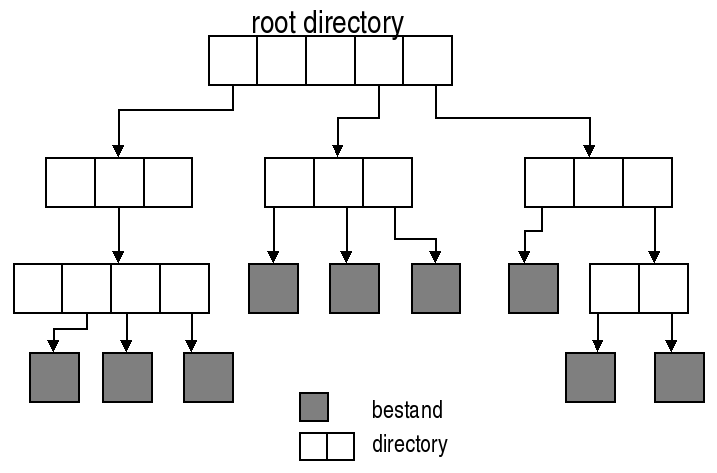
\includegraphics[width=75mm]{images/fig0401.png}
\end{center}
\caption{Boomstructuur}
\label{boomstructuur}
\end{figure}

We kunnen ook stellen dat ieder bestand vanop ieder hoger
niveau in de structuur vanuit juist \'e\'en directory bereikbaar is. We
gebruiken de term boomstructuur, omdat deze structuur zich vertakt
als een boom. In een boom is er naar ieder blad ook slechts \'e\'en
uniek pad van takken. Naar analogie met een boom wordt de directory
van waaruit de structuur vertrekt vaak wortel of \emph{root
directory} genoemd.

\subsubsection{Algemene structuur}

Wanneer we toch meer dan \'e\'en pad naar een bestand toelaten
krijgen we een \emph{algemene structuur}. Dit betekent
dat een bestand een element van twee verschillende directories kan
zijn, of dat een directory een subdirectory is van twee of meer
directories.

\begin{figure}
\begin{center}
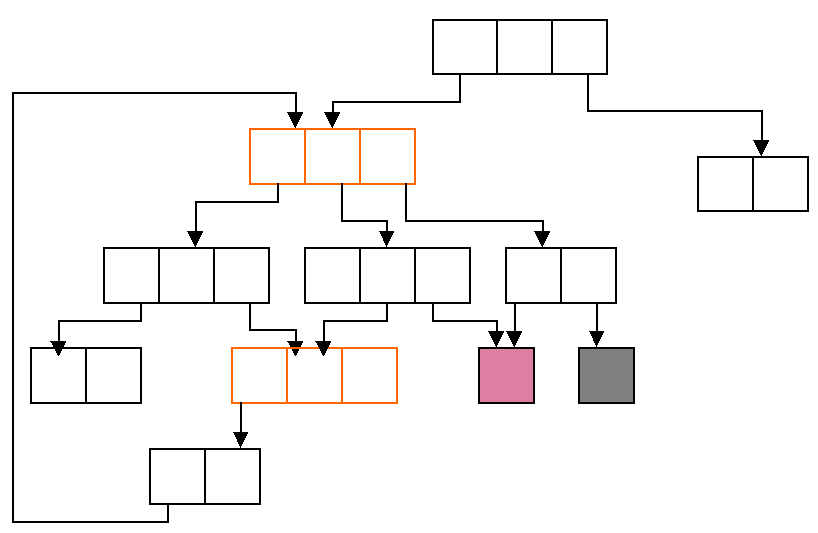
\includegraphics[width=75mm]{images/fig0402.png}
\end{center}
\caption{Algemene structuur}
\label{algstructuur}
\end{figure}

Een dergelijke veralgemening van de structuur kan handig zijn
wanneer een bestand b.v. door meerdere gebruikers wordt gebruikt, of
betrekking heeft op verschillende projecten en het dus niet
eenduidig is waar in de structuur het bestand moet bewaard
worden.

De algemene structuur laat toe dat er lussen gecre\"eerd worden
in het bestandssysteem. Dergelijke lussen veroorzaken heel wat
moeilijkheden. Iedere recursieve operatie op het bestandssysteem,
zoals b.v. het zoeken naar een bestand, zal oneindig doorgaan in
zo'n lus als het recursief algoritme niet detecteert dat het een
bepaalde directory al heeft behandeld.

Een bijkomend probleem betreft het achterblijven van
onbereikbare bestanden in het systeem na het verwijderen van een
directory. Wanneer we vertrekken van de toestand in de vorige
figuur, en we verwijderen een subdirectory van de wortel, krijgen we
de situatie in fig. \ref{problalg1}.

\begin{figure}
\begin{center}
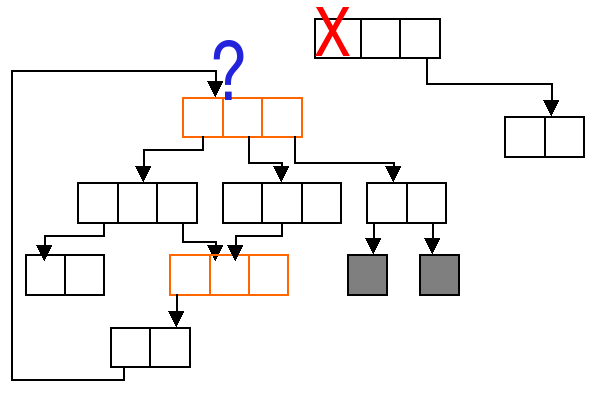
\includegraphics[width=75mm]{images/fig0403.png}
\end{center}
\caption{Problemen bij een algemene structuur}
\label{problalg1}
\end{figure}

De verwijderde subdirectory lijkt nog steeds bereikbaar, omdat
het na het verwijderen van de verwijzing vanuit de wortel nog steeds
een subdirectory is van een andere directory. Op de tekening zien we
echter in \'e\'en oogopslag dat dit geen rol speelt, omdat de directory
die nog naar de verwijderde subdirectory verwijst niet bereikbaar is
vanuit de wortel. Voor het bestandssysteem is het echter verre van
eenvoudig om een dergelijke conclusie te trekken.

Als mogelijke oplossing voor dit probleem zouden we kunnen
beslissen om altijd recursief alle subdirectories te verwijderen,
zelfs al lijken ze nog bereikbaar. Maar dan stuiten we op een tweede
probleem. Stel dat we in fig. \ref{problalg2:a} de aangeduide directory
willen verwijderen.

\begin{figure}
\centering
\begin{subfigure}{.5\textwidth}
  \centering
  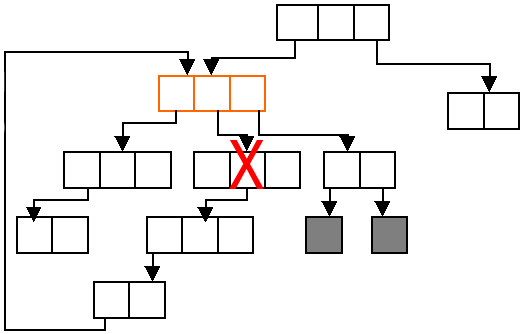
\includegraphics[width=60mm]{images/fig0404a.png}
  \caption{Voor het verwijderen}
  \label{problalg2:a}
\end{subfigure}%
\begin{subfigure}{.5\textwidth}
  \centering
  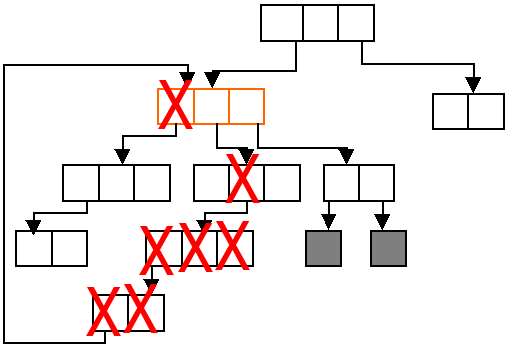
\includegraphics[width=60mm]{images/fig0404b.png}
  \caption{Na het verwijderen}
  \label{problalg2:b}
\end{subfigure}
\caption{Problemen bij een algemene structuur}
\label{problalg2}
\end{figure}


Als we dan alle onderliggende directories recursief
verwijderen, zullen we uiteindelijk een directory verwijderen die
hoger in de hi\"erarchische structuur ligt dan de directory die we
oorspronkelijk wilden verwijderen (fig. \ref{problalg2:b}). Zo zouden we ongewild grote delen
van het bestandssysteem kunnen verwijderen.

Omwille van deze problemen worden dergelijke lussen in het
bestandssysteem zelden toegelaten. Men krijgt dan een acyclische
structuur.

\subsubsection{Acyclische structuur}

De \emph{acyclische structuur} is nog steeds
algemener dan de boomstructuur, maar er mogen geen lussen voorkomen.
Het is dus een beperking van de algemene structuur om de problemen
die lussen kunnen veroorzaken te omzeilen. Lussen vermijden kan op
twee manieren.

We kunnen bij iedere operatie die een lus zou kunnen
veroorzaken een controle uitvoeren. De operatie wordt enkel
toegelaten als er geen lus ontstaat. Zo zijn we zeker dat de
structuur acyclisch zal blijven. Een groot nadeel is natuurlijk dat
de operaties op het bestandssysteem complexer en dus trager
worden.

Een eenvoudigere oplossing is het verbieden van meervoudige
verwijzingen naar directories. Wanneer enkel bestanden vanuit twee
directories kunnen benaderd worden is het onmogelijk een lus te
cre\"eren. Dit beperkt natuurlijk gedeeltelijk de mogelijkheden, maar
maakt de implementatie van een acyclische structuur
eenvoudiger.

Naast de logische structuur die aan de gebruikers
gepresenteerd wordt, moeten we ook nagaan waar de informatie wordt
weggeschreven op de schijf. We streven hierbij naar een systeem dat
de beschikbare capaciteit zo optimaal mogelijk benut, en de
schijftoegang zo snel mogelijk maakt.

\section{Aaneengesloten bestanden}

De meest voor de hand liggende manier om een bestand op de schijf
te zetten is als een aaneengesloten geheel: vanaf een bepaald adres
worden alle bytes van de file achtereenvolgens op de schijf gezet, in
een reeks op elkaar volgende sectoren. We noemen dit een
\emph{aaneengesloten bestand}.\index{aaneengesloten bestand}

\begin{figure}
\begin{center}
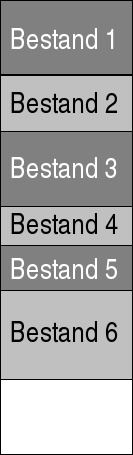
\includegraphics[width=15mm]{images/fig0405.png}
\caption{Aaneengesloten bestanden}
\end{center}
\end{figure}

Dit is een erg eenvoudige werkwijze, maar er ontstaat een
belangrijk probleem: er is een voldoende grote vrije ruimte nodig om het
bestand een plaats te kunnen geven. Zolang er geen bestanden werden
verwijderd en er nog voldoende ruimte beschikbaar is kan een nieuw
bestand gewoon achter het vorige worden geplaatst. Zo werden in het
voorbeeld 6 bestanden aangemaakt.

Naarmate het gebruik van de schijf voortduurt zal er door het
verwijderen van bestanden een steeds groter aantal afzonderlijke vrije
ruimten ontstaan. De omvang van de grootste vrije ruimte zal daarbij ook
steeds kleiner worden. Men zegt dan dat er
\emph{fragmentatie} ontstaat.

\begin{figure}
\begin{center}
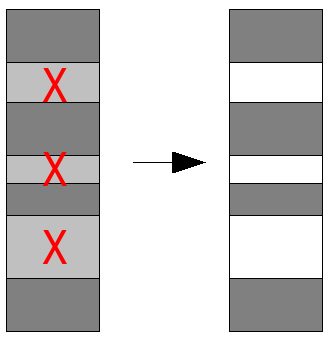
\includegraphics[width=55mm]{images/fig0406.png}
\caption{Fragmentatie}
\end{center}
\end{figure}

Wanneer een bestand toegevoegd moet worden aan een gefragmenteerd
bestandssysteem, moet er gekozen worden waar het bestand op de schijf
geplaatst moet worden. Om een geschikte locatie te kiezen moeten we in
de eerste plaats de grootte van het bestand kennen. Aangezien een
bestand kan groeien naarmate de tijd vordert, is de grootte niet gekend
op het moment dat het bestand aangemaakt wordt. De enige oplossing is om
op de een of andere manier een schatting te maken van de uiteindelijke
grootte.

Als we ervan uitgaan dat we de grootte van het bestand kennen
moeten we nog steeds beslissen in welke vrije ruimte het bestand moet
worden aangemaakt. Om deze keuze te kunnen maken houdt het
bestandssysteem een tabel bij met de adressen en de lengte van alle
vrije ruimten. Er zijn 3 algoritmes om een element van de tabel te
kiezen wanneer een nieuw bestand moet bewaard worden:

Het \emph{First Fit}\index{first fit} algoritme kiest de eerste
vrije ruimte die voldoende groot is voor het bestand. Bij dit algoritme
is de benodigde tijd om de plaats te zoeken natuurlijk minimaal.

Wanneer men gebruik maakt van het \emph{Best Fit}\index{best fit}
algoritme wordt de kleinste vrije ruimte gekozen die groot genoeg is
voor het bestand. \emph{Worst Fit}\index{worst fit} daarentegen kiest de
grootste beschikbare vrije ruimte. Deze algoritmes zullen trager zijn
dan first fit, omdat in dit geval de volledige tabel moet doorzocht
worden. Best and worst fit proberen de fragmentatie tegen te gaan, door
de overblijvende vrije ruimten respectievelijk zo klein of groot
mogelijk te houden.

Best fit probeert dus te vermijden dat een groter bestand dat
eventueel later aangemaakt wordt geen plaats vindt doordat een grote
vrije ruimte verkleind is. Waarschijnlijk past het bestand dat geplaatst
wordt niet helemaal, waardoor best fit vele zeer kleine vrije ruimten
cre\"eert. Worst fit probeert dit net te vermijden. Door het bestand in de
grootste vrije ruimte te plaatsen is de vrije ruimte die overblijft als
het bestand niet exact past ook zo groot mogelijk.

Het belangrijkste voordeel van het werken met aaneengesloten
bestanden is ongetwijfeld de hoge snelheid waarmee met deze bestanden
kan worden gewerkt. Door het gebruik van op elkaar volgende sectoren zal
een bestand zich meestal volledig binnen \'e\'en cylinder van de schijf
bevinden. Er gaat dan geen zoektijd verloren (door de relatief trage
armbewegingen van de schijf).

Een ander voordeel is de mogelijkheid om niet alleen sequenti\"ele,
maar ook directe toegang tot een bepaald deel van het bestand te
krijgen. Als we het startadres $s$ van het bestand, en de blokgrootte $b$
van de schijf kennen (fig. \ref{direct}) kan op eenvoudige wijze het adres $a$ worden berekend
van het blok dat de byte op positie $B$ binnen het bestand bevat\footnote{De
adressen $s$ en $a$ zijn absolute adressen, $B$ is een relatieve verwijzing
binnen het
bestand (voor $B$ beginnen we dus te tellen vanaf $s$).}:

\begin{figure}
\begin{center}
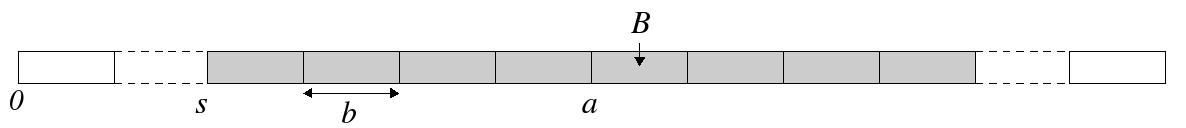
\includegraphics[width=\textwidth]{images/fig0407.png}
\end{center}
\caption{Directe toegang}
\label{direct}
\end{figure}

\begin{displaymath}
a = s + \frac{B}{b}
\end{displaymath}

Tegenover deze voordelen staan enkele ernstige nadelen. Een eerste
moeilijkheid is de verplichting een schatting te geven van de grootte
van elk nieuw bestand. Regelmatig zal bij het schrijven naar een bestand
blijken dat de voorziene ruimte niet volstaat. Dan kan het programma
worden afgebroken om later met een betere schatting te worden hernomen,
ofwel moet het bestandssysteem het programma onderbreken en het reeds
bestaande deel van het bestand naar een grotere vrije ruimte kopi\"eren.
In beide gevallen betekent dit een ernstig prestatieverlies.

Bij het gebruik van aaneengesloten bestanden zorgt fragmentatie\index{fragmentatie}
ervoor dat het bijna onmogelijk is de capaciteit van de schijf volledig
te gebruiken. Na een tijd kan de vrije ruimte op zo'n manier verdeeld
zijn, dat er in het totaal wel voldoende ruimte vrij is om een bepaald
bestand aan te maken, maar niet als een aaneengesloten geheel.

In dat geval is een reorganisatie van de gegevens op het schijf
nodig. zijn. Dit kan gebeuren door alle bestanden op een ander medium te
kopi\"eren, de schijf leeg te maken en er nadien alle bestanden achter
mekaar op terug te plaatsen. Zo wordt opnieuw \'e\'en grote vrije ruimte
gecre\"eerd. Dit \emph{defragmenteren}\index{defragmenteren} kan eventueel ook
zonder tweede medium. Bestanden worden dan verplaatst op de schijf zelf.
Het eenvoudigste algoritme om dit te doen is bovenaan beginnen, en ieder
bestand verplaatsen zodat het aansluit met het vorige. Het resultaat is
een bestandssysteem zonder fragmentatie, maar de defragmentatie is een
tijdrovend proces en dus niet erg handig.

\section{Niet-aaneengesloten bestanden}

Vasthouden aan de ruimtelijke samenhang van een bestand
bemoeilijkt het effici\"ent gebruik van de beschikbare schijvencapaciteit.
De oplossing voor dit probleem kan gevonden worden in het verdelen van
het bestand in kleinere stukken. Zo kan zelfs bij een sterk
gefragmenteerde schijf elke kleine vrije ruimte worden benut om er een
dergelijk stukje van een bestand te plaatsen.

Het gevolg is natuurlijk dat delen van eenzelfde bestand over de
schijf zullen worden verspreid. Als we met deze bestanden werken moet de
lees/schrijfkop zich vaak verplaatsen, wat erg tijdrovend is. Het
verdelen van bestanden gebeurt natuurlijk enkel wanneer er sprake is van
fragmentatie waardoor het niet meer mogelijk is het bestand
aaneengesloten te plaatsen.

Fragmentatie zal dus altijd een nadelige invloed hebben op het
gebruik van opslagmedia. Bij aaneengesloten bestanden leidt fragmentatie
tot een onvolledig gebruik van de capaciteit, en bij niet-aaneengesloten
bestanden veroorzaakt het vertraging in de bestandstoegang. In beide
gevallen is het nuttig het bestandssysteem regelmatig te
defragmenteren.

\subsection{Blokken}

De kleinst mogelijke eenheid waarin we een bestand kunnen
opsplitsen is natuurlijk een sector. Kleinere hoeveelheden gegevens
zijn niet adresseerbaar op een schijf. Vaak wordt echter een grotere
eenheid gebruikt. Het bestandssysteem groepeert een aantal sectoren in
een \emph{blok}\index{blok}, ook soms
\emph{cluster}\index{cluster} genoemd. Binnen het bestandssysteem
worden de adressen van blokken gebruikt, die dan vertaald worden naar
de adressen van de juiste sectoren.

Hoe groot moeten de gebruikte blokken zijn? Een verdeling in
grotere eenheden zorgt ervoor dat het bestand in minder delen
gesplitst wordt. Hierdoor wordt het bestand minder sterk verspreid,
dus moet de leeskop van de schijf minder verplaatsingen maken. De
toegangssnelheid is dus hoger bij grotere blokken. Bovendien zal de
adresinformatie die we nodig hebben om de verschillende delen van het
bestand terug te vinden, kleiner zijn omdat het aantal delen kleiner
is.

Kleinere eenheden hebben dan weer als voordeel dat het
plaatsverlies aan \emph{interne fragmentatie}\index{interne fragmentatie} kleiner
zal zijn. Bij het verdelen van een bestand over een aantal blokken zal
het laatste blok zelden volledig gevuld zijn. Het laatste stuk van dit
laatste blok is onbruikbaar om andere gegevens op te slaan, en gaat
dus verloren. Wanneer b.v. een bestand van 5KB verdeeld wordt over
blokken van 4KB, gaat 3KB aan schijfruimte verloren. Gemiddeld zal bij
ieder bestand een half blok verloren gaan.

Bij de keuze van een blokgrootte moet dus een evenwicht gevonden
worden tussen de toegangssnelheid en het plaatsverlies. Dit is niet
eenvoudig omdat er vele factoren een rol spelen. Het verwachte aantal
bestanden en hun gemiddelde grootte bepalen b.v. mee hoe groot het
effect van de interne fragmentatie zal zijn.

Wanneer we bestanden opsplitsen moet het bestandssysteem
natuurlijk ook bijhouden waar de verschillende delen van een bestand
opgeslagen zijn. We bespreken drie manieren waarop het bestandssysteem
deze boekhouding kan bijhouden, en gaan opnieuw na wat de invloed is
op de toegangssnelheid en de plaatseffici\"entie. We mogen ook niet
vergeten te registreren welke blokken op de schijf niet in gebruik
zijn, zodat we blokken vinden wanneer b.v. een nieuw bestand moet
worden aangemaakt.

\subsection{Bestanden als gelinkte lijsten}

Een eerste mogelijkheid om niet-aaneengesloten bestanden te
beschrijven is het gebruik van gelinkte lijsten: de file descriptor
bevat het adres van het eerste blok van het bestand, en elk blok bevat
een verwijzing of pointer naar het volgende blok. Het laatste blok van
het bestand bevat een speciale pointer die aangeeft dat de lijst
stopt, soms nul-pointer genoemd.

\begin{figure}
\begin{center}
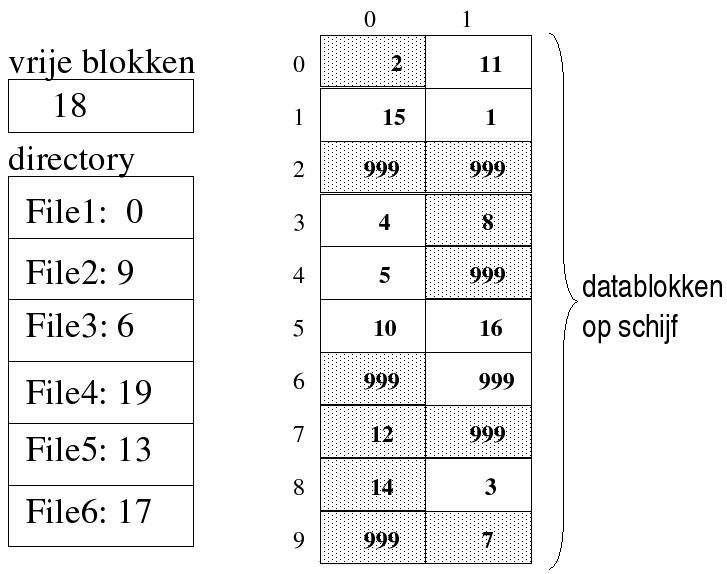
\includegraphics[width=100mm]{images/fig0408.png}
\caption{Bestanden als gelinkte lijsten van blokken}
\end{center}
\label{linklijst}
\end{figure}

Het voorbeeld in fig. \ref{linklijst} bevat een directory zes bestanden. Bij ieder
bestand wordt het adres van het eerste blok bijgehouden. In dat blok
staat het adres van het volgende blok, ofwel '999' dat de nul-pointer
voorstelt.

De blokken waarover File5 verspreid is zijn dus: 13, 8 en
14.

De vrije blokken worden ook d.m.v. een gelinkte lijst
bijgehouden. Ieder vrij blok bevat het adres van het volgende vrije
blok.

Het belangrijkste voordeel van deze methode is dat de
adresinformatie weinig plaats inneemt. In een bestandsbeschrijving
moet maar \'e\'en adres bijgehouden worden, dat van het eerste blok. Dit
zorgt ervoor dat de bestandsbeschrijvingen klein blijven. Ze zijn ook
allemaal even groot, onafhankelijk van de grootte van het
bestand.

Het grootste bezwaar tegen het werken met gelinkte lijsten is
ongetwijfeld de vaststelling dat directe toegang hier niet mogelijk
is. De enige manier om bij een bepaald deel van een bestand te komen
is immers de ketting van verwijzingen te volgen tot bij de gezochte
plaats. Daartoe moeten alle voorafgaande blokken \'e\'en na \'e\'en worden
ingelezen, zodat er eigenlijk sprake is van sequenti\"ele toegang.
Bovendien kunnen de opeenvolgende blokken sterk verspreid zijn over de
schijf, waardoor de toegangssnelheid erg laag kan liggen.

\begin{figure}
\begin{center}
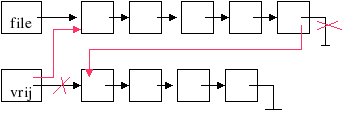
\includegraphics[width=70mm]{images/fig0409.png}
\end{center}
\caption{Gelinkte lijst met verwijzing naar lege blokken}
\label{linklijsteff}
\end{figure}

We kunnen de structuur effici\"enter maken door enkele
aanpassingen, zoals aangegeven in fig. \ref{linklijsteff}. Het verwijderen van een bestand verloopt erg traag omdat
de ketting van alle blokken doorlopen moet worden om de nul-pointer te
vervangen door een verwijzing naar het eerste blok van de lijst met
vrije blokken\footnote{Omgekeerd zou ook kunnen, we zouden de nul-pointer in het
laatste blok uit de lijst van vrije blokken kunnen vervangen door een verwijzing
naar het eerste blok van het verwijderde bestand. In het algemeen zal de
hoeveelheid vrije ruimte echter groter zijn dan het te verwijderen bestand,
waardoor het op die manier nog trager zou gaan.}

Door in de bestandsbeschrijving ook een pointer naar het laatste
blok bij te houden kunnen we het verwijderen van een bestand
versnellen.

Wanneer er iets misloopt met een verwijzing gaat een deel van
een bestand verloren, of kan een bestand soms onterecht verwijzen naar
een deel van een ander bestand. Wanneer het beschadigde bestand
verwijderd wordt gaat ook een deel van dit andere bestand verloren.
Het is ook mogelijk dat er schijfruimte verloren gaat als er iets
misloopt met de lijst met vrije blokken.

Om dergelijke problemen op te vangen wordt soms gewerkt met een
\emph{dubbel gelinkte lijst}\index{dubbel gelinkte lijst}, waarin ieder blok ook
verwijst naar het vorige blok in de lijst (zie fig. \ref{dubellink}). Een foutieve verwijzing kan
dan hersteld worden door de lijst van achter naar voor te
doorlopen.

\begin{figure}
\begin{center}
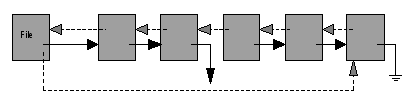
\includegraphics[width=90mm]{images/fig0410.png}
\caption{Dubbel gelinkte lijst}
\label{dubellink}
\end{center}
\end{figure}


\subsection{Bestanden met indexblokken}

De onmogelijkheid tot directe toegang bij een gelinkte lijst van
blokken wordt veroorzaakt door de verspreiding van de adresinformatie
doorheen het bestand. Dit probleem kan worden opgelost door de
adressen van de verschillende onderdelen van een bestand te verzamelen
in een speciaal daarvoor voorbehouden blok op schijf: een
\emph{indexblok}\index{indexblok}. In de file descriptor zal dan als
plaatsaanduiding het adres van dit indexblok worden opgenomen.

\begin{figure}
\begin{center}
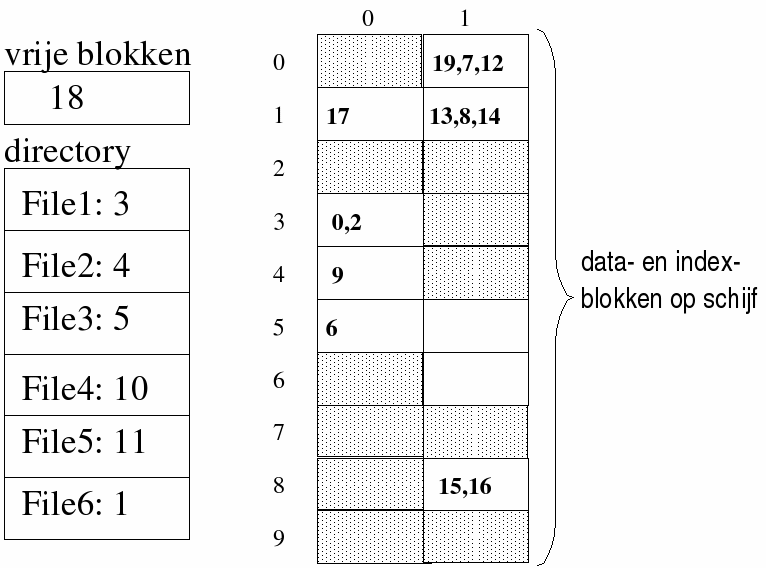
\includegraphics[width=120mm]{images/fig0411.png}
\caption{Bestanden met indexblokken}
\label{indexblokken}
\end{center}
\end{figure}

In fig. \ref{indexblokken} bevat iedere bestandsbeschrijving in de
directory het adres van een indexblok. De indexblokken zijn dus 3, 4,
5, 10, 11 en 1.

Elk van deze indexblokken bevat de adressen van de blokken met
de eigenlijke gegevens van het bestand.

Ook de vrije blokken worden bijgehouden in een indexblok
(18).

Indien \'e\'en blok niet volstaat om alle adresinformatie op te
slaan zijn er verschillende oplossingen. Men kan een gelinkte lijst
van indexblokken cre\"eren, of men kan een \emph{hi\"erarchische
index-structuur} opbouwen. Hierbij verwijst het eerste
indexblok niet naar delen van het bestand, maar naar indexblokken die
de adressen van de blokken met gegevens bevatten. Men kan een
dergelijke hi\"erarchische structuur zo diep maken als men wil.

Het grootste voordeel van een structuur met indexblokken is de
toegangssnelheid. Wanneer een bestand geopend wordt kan het indexblok
volledig in het geheugen geladen worden. Hierdoor is directe toegang
mogelijk, in tegenstelling tot de structuur met gelinkte lijsten.
Zelfs bij seri\"ele toegang is er een kleine snelheidswinst, omdat er
niet moet gewacht worden tot het bestandssysteem het adres van het
volgende blok uit het vorige blok gelezen heeft kunnen er meerdere
leesopdrachten tegelijk aan de schijf doorgegeven worden.

Een nadeel van indexblokken is dat ze schijfruimte innemen. Het
gegeven voorbeeld voor gelinkte lijsten en indexblokken is hetzelfde,
maar in het eerste geval hadden we 9 vrije blokken over en bij
indexblokken zijn er dat maar 2. Dit komt omdat er per bestand \'e\'en
blok extra nodig is: het indexblok.

Dit plaatsverlies is vooral groot wanneer er veel kleine
bestanden voorkomen in het systeem. Wanneer een bestand maar \'e\'en blok
groot is neemt het 2 keer zoveel plaats in op de schijf door het
indexblok. Hoe groter het bestand, hoe kleiner het relatieve verlies.
Op een bestand van 100 blokken is \'e\'en indexblok een minder groot
verlies.

Daarom wordt in de bestandsbeschrijving vaak plaats voorzien
voor een klein aantal adressen van blokken van het bestand. Als de
hoeveelheid benodigde blokken onder dit aantal blijft, moet er geen
indexblok gebruikt worden. De toegang tot deze kleine bestanden is dan
ook iets sneller omdat er \'e\'en schijftoegang uitgespaard wordt.

De toegangssnelheid kan verder worden geoptimaliseerd door
zogenaamde extents te gebruiken in plaats van afzonderlijke blokken.
Een \emph{extent}\index{extent} is een verzameling opeenvolgende
blokken op de schijf (fig. \ref{extents}). Hierdoor zullen grotere delen van een file op
een zelfde plaats van de schijf terechtkomen, zodat het lezen of
schrijven minder onderbroken hoeft te worden voor een verplaatsing van
de leeskop. Indien de extents gemiddeld voldoende groot zijn zal ook
minder informatie moeten worden opgeslagen in de indexblok. Het adres
van het eerste blok en de lengte van de extent zijn voldoende. In de
figuur verwijst indexblok 3 naar 2 extents.

\begin{figure}
\begin{center}
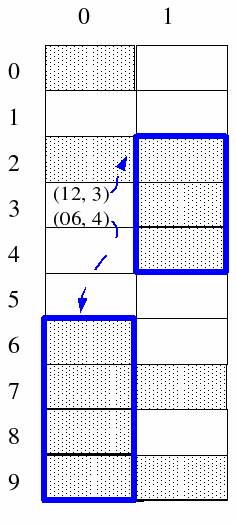
\includegraphics[width=35mm]{images/fig0412.png}
\caption{Extents}
\label{extents}
\end{center}
\end{figure}


\subsection{Bestanden beschrijven in een file map}

In de derde oplossing beschrijven we de inhoud van de schijf in
een aparte tabel. In deze tabel, de \emph{file map}\index{file map},
wordt voor ieder blok van de schijf aangegeven of het vrij is, en
indien niet, tot welk bestand het behoort.

De eenvoudigste versie van een file map is een bitvector\index{bitvector}, die
voor ieder blok aangeeft of het vrij is of niet. Met ieder blok komt
een bit overeen, 1 betekent dat het blok in gebruik is, 0 betekent dat
het blok beschikbaar is. Deze structuur zou kunnen gebruikt worden
i.p.v. een gelinkte lijst of indexblokken met vrije blokken.
Vergeleken met indexblokken zorgt zo'n bitvector van vrije blokken
voor minder plaatsverlies. De vaste lengte van de bitvector (1 bit per
blok) is wel nadelig als er weinig vrije blokken zijn. Als er een vrij
blok is ziet de bitvector er namelijk als volgt uit:
111...1110111...111.

Met elk blok (of andere eenheid) komt een element van de tabel
overeen. Een vrij blok wordt aangeduid door een speciale code. De
elementen, behorend bij de blokken die samen een bestand vormen,
bevatten pointers zodat ze een gelinkte lijst vormen. Het laatste
element in de lijst bevat een code om het einde van het bestand aan te
geven. De plaatsaanduiding in de file descriptor bestaat uit de index
van het element dat overeenstemt met het eerste blok in de
file.

\begin{figure}
\begin{center}
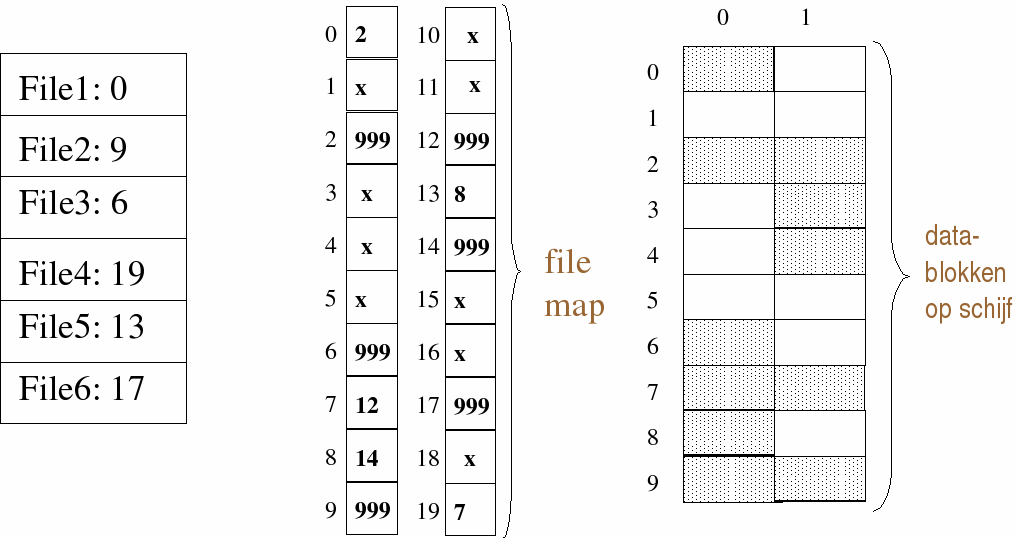
\includegraphics[width=\textwidth]{images/fig0413.png}
\caption{File map}
\label{filemap}
\end{center}
\end{figure}

In fig. \ref{filemap} wordt opnieuw hetzelfde voorbeeld als bij de twee vorige
structuren getoond. De file descriptor van File5 verwijst nu naar het element
op positie 13 in de file map. Dit leert ons dat het blok op adres 13
het eerste blok van het bestand File5 is, en op positie 13 in de file
map vinden we de index van het volgende blok. Blokken 8 en 14
vervolledigen dus het bestand.

Een groot voordeel van een file map is de mogelijkheid om de
volledige beschrijving van een schijf in het centrale geheugen te
brengen. Dit maakt directe toegang tot de bestanden mogelijk en
bespaart ook telkens het afzonderlijk inlezen van adresinformatie. We
werken eigenlijk weer met een gelinkte lijst, maar nu is de volledige
lijst van adressen al beschikbaar in het werkgeheugen.

Men kan er ook op een eenvoudige wijze voor zorgen dat een
bestand zo goed mogelijk gegroepeerd blijft: de combinatie van de
beschrijving van de met de adresgegevens van het bestand in \'e\'en tabel
laat toe bijkomende ruimte voor het bestand te zoeken in de
onmiddellijke nabijheid van het laatst toegekende blok.

\section{Directories (2)}

Nu we de fysische opslag van bestanden op de schijf bekeken
hebben, keren we nog even terug naar de directories. We weten dat er
verschillende logische structuren zijn, zoals de cyclische en acyclische
hi\"erarchie\"en. Maar ook deze directories moeten ergens op de schijf een
plaats krijgen.

Een directory is een verzameling bestandsbeschrijvingen. Er zijn
verschillende fysische structuren mogelijk om deze
bestandsbeschrijvingen op een schijf op te slaan: een gewone tabel, een
gesorteerde tabel, een hashtabel of een gelinkte lijst. Om een keuze te
kunnen maken beschouwen we vooral de snelheid waarmee bewerkingen in de
directory kunnen worden uitgevoerd. Deze basisbewerkingen zijn het
opzoeken, toevoegen en verwijderen\footnote{Merk op dat het verwijderen van een
bestandsbeschrijving uit een directory veronderstelt dat we de
bestandsbeschrijving eerst zoeken.} van een bestandsbeschrijving uit de
directory.

\subsection{Tabel}

Wanneer we de bestandsbeschrijvingen in een tabel bijhouden, zal
vooral het opzoeken van een bestandsbeschrijving relatief veel tijd
vragen. We moeten de tabel doorlopen tot we het gezochte element
vinden. In het beste geval is het het eerste element, in het slechtste
geval het laatste. Gemiddeld zullen we de halve tabel moeten
doorzoeken.

Het toevoegen van een file descriptor kan zeer snel gebeuren,
aangezien die gewoon achteraan kan bijgeplaatst worden.

\subsection{Gesorteerde tabel}

Om het opzoeken in een tabel te versnellen kan de tabel
gesorteerd worden. Het is dan mogelijk om het binair zoeken toe te
passen: bekijk het middelste element, en dan weet je of het gezochte
element ervoor of erachter ligt. Zo kan je onmiddellijk de helft van
de tabel negeren, en op dezelfde manier verderzoeken in de
overgebleven helft.

Wanneer de 1000 elementen van een tabel niet gesorteerd zijn
moeten we gemiddeld 500 elementen bekijken vooraleer we het gezochte
element vinden. Bij binair zoeken in een gesorteerde tabel met 1000
elementen vinden we wat we zoeken na het bekijken van slechts 10
elementen\footnote{Je kan dit als volgt berekenen: Aangezien telkens de helft
van de elementen wegvallen hebben we er na het bekijken van 1 element nog 500
over. Na nog een element te bekijken zijn het er nog 250. De reeks is dus: 1000,
500, 250, 125, 63, 32, 16, 8, 4, 2, 1. Na 10 stappen blijft er slechts \'e\'en
element over. Wiskundig gezien berekenen we log2(1000), wat ongeveer gelijk is
aan 9,97.}. Wanneer we een tabel met 1.000.000 elementen binair doorzoeken zijn
20 stappen voldoende, terwijl we gemiddeld er 500.000 elementen zouden moeten
bekijken als de tabel niet gesorteerd zou zijn.

Doordat we de tabel gesorteerd moeten houden zal het toevoegen
van file descriptors natuurlijk wel trager verlopen. We moeten immers
eerst de juiste plaats zoeken. Dit zoeken kan ook binair, maar dan
moeten alle achterliggende elementen nog opgeschoven worden om plaats
te maken voor de nieuwe bestandsbeschrijving. Bij het verwijderen
moeten we de legen plaats opvullen door alle volgende elementen een
plaats naar voor te schuiven.

\subsection{Hashtabel}

Een hashtabel is een structuur die zeer effici\"ent opzoeken
toelaat. De positie in de tabel wordt berekend met behulp van de
hash-functie. In dit geval zal de gekozen hash-functie de bestandsnaam
transformeren in een geheel getal. De bestandsbeschrijving zal dan op
deze positie in de hashtabel bewaard worden. Wanneer we een
bestandsbeschrijving zoeken, berekenen we de hashwaarde van de
bestandsnaam, en we kennen onmiddellijk de positie waarop de gezochte
file descriptor staat.

Een mogelijk probleem zijn \emph{collisions} of
\emph{botsingen}. Wanneer de hash-functie voor twee
verschillende bestandsnamen dezelfde positie teruggeeft spreken we van
een botsing. Dan worden op die plaats in de tabel meestal
verschillende elementen bijgehouden, en moet in deze verzameling
elementen op een klassieke manier gezocht worden. Hoe groter de
hashtabel (dus hoe meer posities, en hoe meer mogelijke uitkomsten
voor de hash-functie), hoe kleiner de kans op een botsing. Het nadeel
is natuurlijk dat er meer plaats verloren gaat voor de grotere
tabel.

In gunstige omstandigheden levert de hash-functie dus
onmiddellijk de plaats van een op te zoeken file descriptor. Ook het
toevoegen of verwijderen van file descriptors kan zeer snel
gebeuren.

\subsection{Gelinkte lijst}

Ook een directory kan bijgehouden worden als een gelinkte lijst.
In de tabel verwijst ieder element naar de positie van het volgende.
We moeten dan alleen de startpositie kennen.

\begin{figure}
\begin{center}
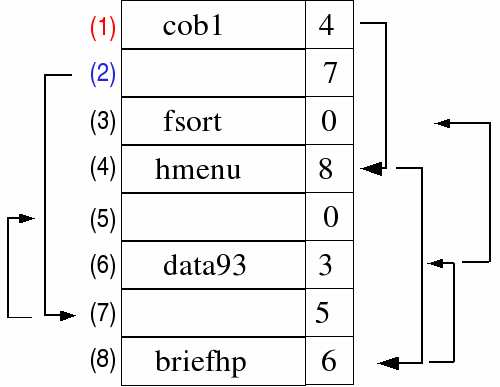
\includegraphics[width=60mm]{images/fig0414.png}
\caption{Directory als gelinkte lijst}
\label{dirlinklijst}
\end{center}
\end{figure}


In fig. \ref{dirlinklijst} is (1) de startpositie voor de directory. (2) is het begin van de lijst met vrije plaatsen in de tabel. Een verwijzing naar 0 geeft het einde van de lijst aan.

Wat betreft het opzoeken van een element in de lijst is deze
structuur te vergelijken met de klassieke tabel. Het moet sequentieel
gebeuren. Zelfs als de elementen van de lijst gesorteerd zouden zijn
is binair zoeken niet zoveel effici\"enter, aangezien we geen
rechtstreekse toegang hebben tot het middelste element.

Bij het toevoegen en verwijderen daarentegen vermijden we het
verschuiven van de achterliggende elementen om plaats te maken of om
een vrijgekomen plaats op te vullen. We kunnen gewoon de verwijzingen
aanpassen, en alle elementen kunnen op hun plaats blijven staan. Het
geringe plaatsverlies door de verwijzing naar de volgende
bestandsbeschrijving levert dus snelheidswinst bij deze
operaties.

\section{Voorbeeld 1: FAT}

Het FAT-bestandssysteem\index{FAT-bestandssysteem} is het oorspronkelijke bestandssysteem van
het MS-DOS besturingssysteem. Voor steeds groter wordende harde schijven
raadt Microsoft vanaf Windows NT het NTFS bestandssysteem aan, maar FAT
wordt nog steeds gebruikt op diskettes en allerlei USB-opslagmedia zoals
MP3-spelers en digitale camera's.

\subsection{File Allocation Table}

\emph{FAT} staat voor \emph{File Allocation
Table}\index{file allocation table}. Deze FAT is een file map met daarin de nodige
informatie over ieder blok van de schijf. Een FAT-partitie bevat een
boot sector, 2 kopie\"en van de FAT, en een datagebied dat de
directories en bestanden bevat.

In de FAT wordt voor ieder blok van de schijf \'e\'en van vijf
mogelijkheden bijgehouden. Wanneer het blok een onderdeel van een
bestand is bevat het overeenkomstige FAT-element het adres van het
volgende blok van het bestand, zoals hierboven algemeen beschreven
voor file maps. Het laatste blok van een bestand wordt aangeduid met
de End Of File (EOF)-code 0xFFFF, en een vrij blok met 0x0000. Er zijn
ook codes om gereserveerde en slechte blokken aan te duiden.

Er zijn verschillende varianten van het FAT bestandssysteem. De
oorspronkelijke versie wordt nu FAT12 genoemd, naast de nieuwere
versies FAT16 en FAT32. Het getal in de naam van deze systemen duidt
aan hoeveel bits er gebruikt worden voor ieder element in de FAT. In
een FAT12 systeem bevat ieder element van de FAT dus 12 bits.

Het aantal bits dat een FAT-element bevat bepaalt welke adressen
gebruikt kunnen worden voor de blokken. In een FAT12-tabel zijn er
voor ieder element $2^{12}$ of $4096$
mogelijkheden. Dat betekent dat er maximum 4096 verschillende adressen
kunnen gebruikt worden. Wanneer de blokgrootte 512B (1 sector) is,
betekent dit dat er niet meer dan 4096 x 512 B of 2MB kunnen
geadresseerd worden. Omwille van deze limiet op de schijfgrootte was
het nodig om de nieuwe versies FAT16 en FAT32 in te voeren. Met
dezelfde blokgrootte kan een FAT32 systeem een schijf van 2TB
adresseren. We stellen dus vast dat de maximale adresseerbare
schijfcapaciteit bepaald wordt door het beschikbaar aantal bits voor
het adres, maar dat ook de blokgrootte een rol speelt. Hoe groter de
blokken, hoe groter de maximale capaciteit.

De totale grootte van de FAT-tabel speelt ook een belangrijke
rol, aangezien we omwille van de performantie de volledige tabel in
het werkgeheugen willen houden. Aangezien bij een FAT12
bestandssysteem $2^{12}$ of $4096$ verschillende
adressen mogelijk zijn, is dit ook het maximaal aantal elementen in de
tabel (1 element per blok). De grootte van de tabel is dan
$2^{12}x12$ bits, dus $49152$ bits of 6KB. Voor
FAT32 wordt dit $2^{32}x32$ bits, wat
overeenkomt met 16GB. Het is duidelijk niet haalbaar om een
dergelijke tabel in het werkgeheugen bij te houden.

Door de blokgrootte te verhogen kunnen we dus ofwel zorgen voor
een grotere adresseerbare schijfcapaciteit, of voor een kleinere
FAT-tabel. De volgende tabel geeft de standaard blokgrootte voor
FAT-bestandssystemen in Windows XP:

\begin{center}
\begin{tabular}{|l|l|}
\hline
Partitiegrootte  & Blokgrootte \\
\hline
33MB - 64MB      & 512B \\
65MB - 128MB     & 1KB \\
129MB - 256MB    & 2KB \\
257MB - 8GB      & 4KB \\
8GB - 16GB       & 8KB \\
16GB - 32GB      & 16KB \\
$>$ 33GB         & Niet ondersteund\\
\hline
\end{tabular}
\end{center}

Wanneer je dus een partitie van 12GB als FAT32 formatteert in
Windows XP, zullen er blokken van 8KB gebruikt worden. Dit betekent
dat ieder blok 16 sectoren op de schijf inneemt. Merk op dat je voor
partities van meer dan 32GB het NTFS bestandssysteem moet gebruiken
in Windows XP.

\subsection{Directories}

De logische structuur van het FAT bestandssysteem is een
boomstructuur. Fysisch wordt een directory voorgesteld als een gewone
tabel. Deze tabel wordt op dezelfde manier opgeslagen op de schijf als
een gewoon bestand: de blokken waarop de directory-tabel staan worden
via een gelinkte lijst in de FAT bijgehouden.

In FAT12 en FAT16 staat de root-directory onmiddellijk na de 2
kopie\"en van de FAT. In FAT32 is dit niet meer verplicht. In de
directory-tabel neemt iedere bestandsbeschrijving 32 bytes in. De
betekenis van deze 32 bytes wordt hieronder aangegeven.

\begin{center}
\begin{tabular}{|l|l|l|}
\hline
Veld                              & Positie & Lengte \\
\hline
Naam                              & 0       & 8      \\
Extensie                          & 8       & 3      \\
Attributen                        & 11      & 1      \\
Tijdstip Creatie                  & 12      & 1      \\
Hoogste bytes startadres          & 20      & 2      \\
Startadres (FAT32: laagste bytes) & 26      & 2      \\
Grootte                           & 28      & 4      \\
\hline
\end{tabular}
\end{center}

We zien hier onmiddellijk waarom bestandsnamen in MS-DOS beperkt
zijn tot 8 karakters voor de naam en 3 karakters voor een
extensie.

Het attributen-veld verdient nog wat aandacht. Elk van de 8 bits
komt over\'e\'en met een bepaald attribuut, en duidt aan of dit attribuut
op het element van de directory van toepassing is. E\'en van de
attributen is het 'directory' attribuut. Als hier een '1' staat
beschijft dit element een subdirectory, anders een bestand. Voor ieder
bestand zijn er de read-only, hidden, system en archive
attributen.

\begin{figure}
\begin{center}
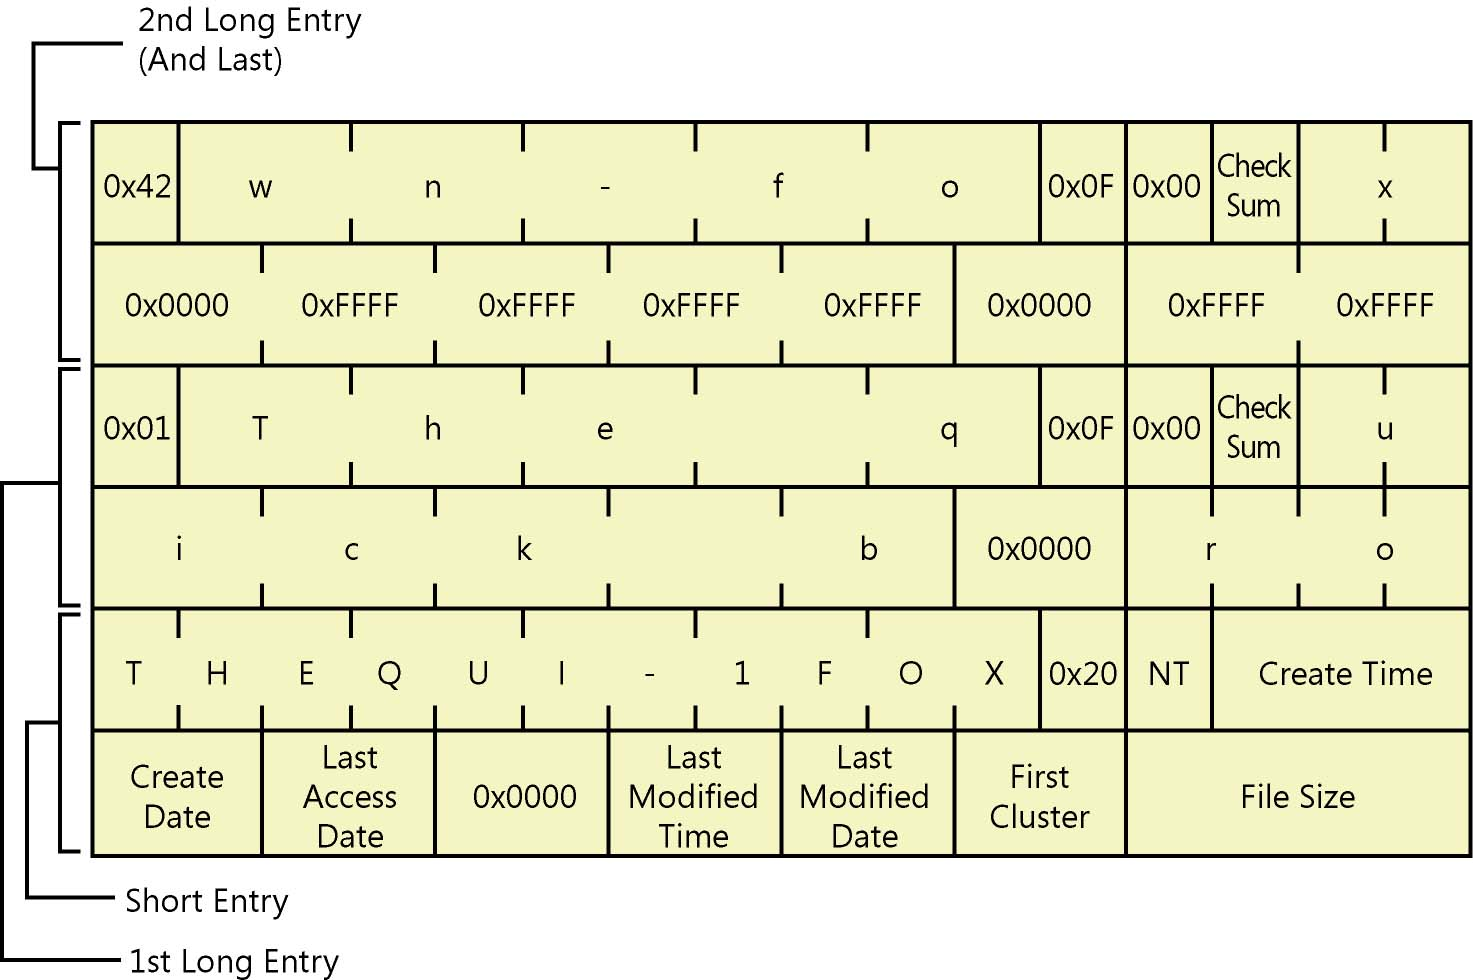
\includegraphics[width=\textwidth]{images/fig0415.jpg}
\caption{Lange bestandsnamen in FAT \tiny{afbeelding uit ``Windows XP Professional Resource Kit''}}
\label{fatlangnaam}
\end{center}
\end{figure}


Het Volume Label attribuut wordt normaal slechts voor \'e\'en
speciaal element van de root directory gebruikt. In iedere andere
context negeert MS-DOS dit bestanden waarbij dit attribuut op '1'
staat. Hiervan is handig gebruik gemaakt om in Windows de mogelijkheid
te voorzien om langere bestandsnamen te gebruiken in
FAT-bestandssystemen (zie fig. \ref{fatlangnaam}).

De lange naam wordt verspreid over bepaalde delen van meerdere
tabelelementen. Het volume-attribuut van deze elementen wordt op 1
gezet, zodat MS-DOS ze negeert. MS-DOS gebruikt nog steeds een
verkorte versie van de naam die in de eigenlijke bestandsbeschrijving
bijgehouden wordt.

\section{Voorbeeld 2: NTFS}

% alle details op:
% https://technet.microsoft.com/en-us/library/cc781134(v=ws.10).aspx

NTFS\index{NTFS-bestandssysteem} staat voor New Technology File System. Het is het standaard
bestandssysteem voor Windows NT, 2000, XP en hoger. Het lost
enkele problemen met FAT op en bevat heel wat extra
functionaliteit.

NTFS bestandsnamen kunnen 255 tekens lang zijn, en de tekens
worden m.b.v. unicode bewaard. Hierdoor kunnen naast het gewone Westerse
alfabet allerlei andere tekens gebruikt worden.

\subsection{Master File Table}

NTFS maakt gebruik van een \emph{Master File
Table}\index{master file table} (\emph{MFT}). In deze tabel wordt
voor ieder bestand \'e\'en bestandsbeschrijving bijgehouden. Deze
beschrijving bevat naast de bestandsnaam, de grootte en de
toegangsdata informatie over de toegangsrechten tot het
bestand.

In tegenstelling tot de File Allocation Table in het FAT-systeem
is de MFT dus geen file map. De MFT bevat \'e\'en record per bestand, en
niet \'e\'en record per blok op de schijf. Hierdoor is de grootte van de
MFT variabel. Standaard wordt 12,5\% van de partitie voorzien voor de
MFT, en de overige 87,5\% is beschikbaar voor gegevens. Wanneer het
datagebied echter vol is, en de MFT neemt niet de voorziene 12,5\% van
de partitie in kan die ook voor data gebruikt worden.

\begin{figure}
\begin{center}
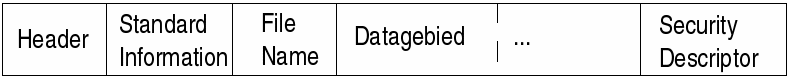
\includegraphics[width=100mm]{images/fig0416.png}
\caption{MFT-record}
\label{mftrecord}
\end{center}
\end{figure}

Een record in de MFT bevat attributen. In fig. \ref{mftrecord} worden de
attributen getoond die voor ieder bestand aanwezig zijn. Welke overige attributen
gebruikt worden staat niet vast in de specificatie van NTFS. De
gebruikte attributen op de partitie worden in het systeembestand
\$AttrDef bijgehouden.

De standaardinformatie omvat de grootte van het bestand, de
toegangsdatums en andere eigenschappen. De toegangsrechten worden
bewaard in de security descriptor\index{security descriptor}. Omdat attributen geen vaste lengte
hebben is er een hoofding nodig die de structuur van het record
beschrijft.

Wanneer de inhoud van een attribuut te groot wordt om in het
MFT-record te bewaren wordt het attribuut non-resident gemaakt. Dit
betekent dat de inhoud van het attribuut in vrije blokken in het
datagebied bewaard wordt, en dat het MFT-record een verwijzing naar
deze blokken bevat.

\begin{figure}
\begin{center}
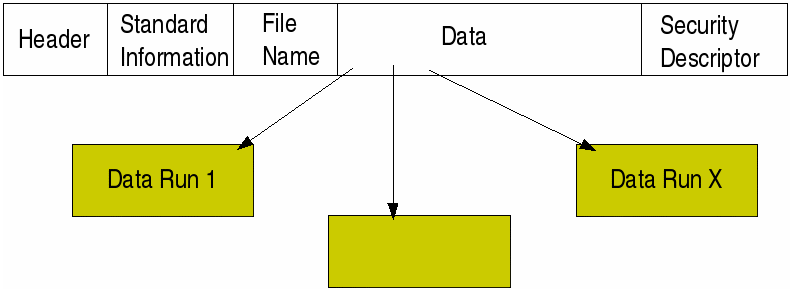
\includegraphics[width=100mm]{images/fig0417.png}
\caption{Data Runs}
\label{dataruns}
\end{center}
\end{figure}

Het data-attribuut in een MFT-record bevat verwijzingen naar
blokken in het datagebied. We kunnen het data-attribuut dus beschouwen
als een indexblok. Om de toegangssnelheid te verhogen en de
hoeveelheid adresinformatie te beperken wordt gebruik gemaakt van
extents, die in de context van NTFS vaak data runs of streams\index{stream} genoemd
worden (fig. \ref{dataruns}).

Voor kleine bestanden wordt de inhoud van het bestand zelf
binnen het data-attribuut in het MFT-record opgeslagen. Dit zorgt
ervoor dat met dergelijke bestanden zeer snel gewerkt kan worden. Zo
gauw het bestand is opgezocht is directe toegang mogelijk zonder
verdere schijftoegangen. Dit gebeurt typisch voor bestanden die
kleiner zijn dan 900 bytes. Als we dit geval als standaard
beschouwen, kunnen we zeggen dat als een bestand te groot wordt het
data-attribuut non-resident gemaakt wordt.

Wanneer een bestand zo groot wordt dat de verschillende data
runs niet meer binnen het data-attribuut kunnen beschreven worden is
het mogelijk om het data-attribuut zelf buiten het MFT-record op te
slaan (fig. \ref{nonresdata}). Deze structuur kan nog verder uitgebreid worden zodat de ruimte
van het data-attribuut in de MFT-record een indirect indexblok
wordt.

\begin{figure}
\begin{center}
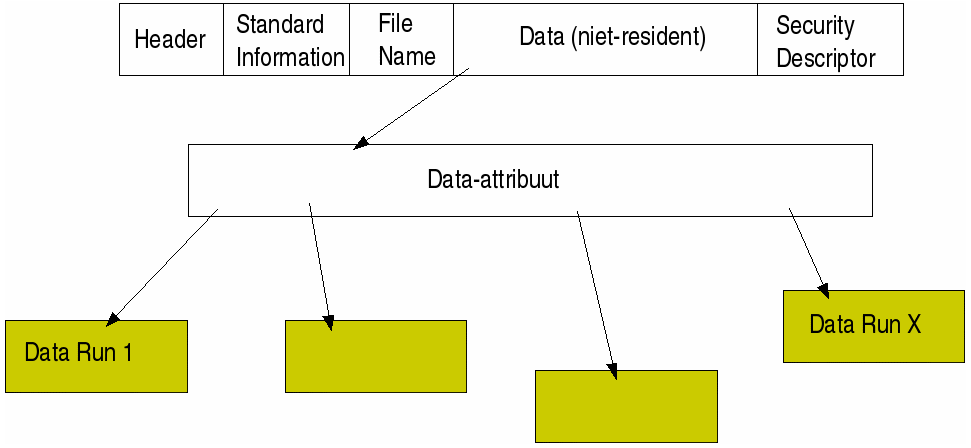
\includegraphics[width=120mm]{images/fig0418.png}
\caption{Niet-resident data-attribuut}
\label{nonresdata}
\end{center}
\end{figure}

Door deze flexibele structuur is er bij NTFS geen sprake van een
maximale bestandsgrootte. In theorie kan \'e\'en bestand de beschikbare
capaciteit van de volledige partitie innemen.

\subsection{Directories}

De logische structuur van NTFS is een boomstructuur, net als bij
FAT. Voor directories wordt ook een record in de MFT aangemaakt. Een
directory-record heeft extra attributen die verwijzingen bevatten naar
de bestanden en subdirectories. Net als bij gewone bestanden worden
deze gegevens voor een kleine directory in het record
bijgehouden.

De fysische structuur van de inhoud van een directory wordt
bijgehouden m.b.v. B-bomen. Dit zijn vrij ingewikkelde gebalanceerde
en gesorteerde boomvormige gegevensstructuren die snel opzoeken en
toevoegen van elementen toelaten.

\section{Voorbeeld 3: Second Extended File System}

Hoewel je bij het installeren van een Linux-distributie de keuze krijgt
uit een hele lijst met bestandssystemen om de partities te formatteren,
wordt het \emph{Extended File System}\index{extended file system} vaak beschouwd als het standaard-bestandssysteem
voor Linux. De meest recente versie is het Fourth Extended File System of ext4. We zullen
ons hier beperken tot een analyse van de werking van ext2.

\subsection{Inodes}

Net zoals Linux zelf is het Extended File System, en dus ook de opvolgers, gebaseerd op
Unix. De algemene structuur van een ext2-partitie is dan ook dezelfde als bij het
Unix File System. De blokken van de schijf kunnen worden ingedeeld in 4 soorten:

\begin{itemize}
\item Bootblok
\item Superblok
\item Inodeblokken
\item Datablokken
\end{itemize}

In het \emph{bootblok}\index{bootblok} staat bootstrap code die het besturingssysteem moet laden en opstarten.
Het heeft geen specifieke functie in het bestandssysteem. Het \emph{superblok}\index{superblok} bevat globale
gegevens over het bestandssysteem, en enkele instellingen.

Met ieder bestand in ext2 wordt een gegevensstructuur geassoci\"eerd, die \emph{inode}\index{inode} wordt genoemd.
Hierin vinden we alle metadata en de verwijzingen naar de datablokken waarin de inhoud
van het bestand opgeslagen is. Achter het superblok staat een lijst met inodeblokken\index{inodeblok}, soms ook
I-list genoemd. De overige blokken in het bestandssysteem worden gebruikt om de inhoud van bestanden
in weg te schrijven.

Aangezien de broncode van Linux vrij beschikbaar is, kunnen we de eigenlijke structuur van een inode
bekijken. Linux is geschreven in C, en de inode struct\footnote{Een struct in C kan je vergelijken
met een vereenvoudigde klasse uit Java. Een struct in C bevat enkel dataleden, en geen methodes.}
wordt gedefini\"eerd in het bestand \verb|include/ext2_fs.h|. Dit komt uit de broncode van versie 1.0
van de Linux kernel (1994):

\begin{verbatim}
/*
 * Structure of an inode on the disk
 */
struct ext2_inode {
    unsigned short i_mode;      /* File mode */
    unsigned short i_uid;       /* Owner Uid */
    unsigned long  i_size;      /* Size in bytes */
    unsigned long  i_atime;     /* Access time */
    unsigned long  i_ctime;     /* Creation time */
    unsigned long  i_mtime;     /* Modification time */
    unsigned long  i_dtime;     /* Deletion Time */
    unsigned short i_gid;       /* Group Id */
    unsigned short i_links_count;   /* Links count */
    unsigned long  i_blocks;    /* Blocks count */
    unsigned long  i_flags;     /* File flags */
    unsigned long  i_reserved1;
    unsigned long  i_block[EXT2_N_BLOCKS];/* Pointers to blocks */
    unsigned long  i_version;   /* File version (for NFS) */
    unsigned long  i_file_acl;  /* File ACL */
    unsigned long  i_dir_acl;   /* Directory ACL */
    unsigned long  i_faddr;     /* Fragment address */
    unsigned char  i_frag;      /* Fragment number */
    unsigned char  i_fsize;     /* Fragment size */
    unsigned short i_pad1;
    unsigned long  i_reserved2[2];
};
\end{verbatim}

Een inode bevat dus allerlei gegevens, waaronder b.v. de eigenaar en toegangsrechten. Merk op
dat de bestandsnaam niet in de inode wordt bewaard. De bestandsnamen vinden we in de directories,
samen met een verwijzing naar de inode. Dit verschilt van b.v. FAT, waarbij de volledige
bestandsbeschrijving in de directory wordt bijgehouden.

\begin{verbatim}
/*
 * Structure of a directory entry
 */
#define EXT2_NAME_LEN 255

struct ext2_dir_entry {
    unsigned long  inode;           /* Inode number */
    unsigned short rec_len;         /* Directory entry length */
    unsigned short name_len;        /* Name length */
    char           name[EXT2_NAME_LEN]; /* File name */
};
\end{verbatim}

Zoals je in de code kan zien kan een ext2-bestandsnaam kan tot 255 tekens bevatten. Zoals gezegd is
een directory een bestand met daarin een lijst van bestandsnamen gekoppeld aan een inode. Omdat dergelijke
lange namen niet vaak voorkomen werd gekozen voor directory-elementen met variabele lengte. Het inode-nummer
wordt opgeslagen, gevolgd door 2 variabelen die resp. de lengte van de entry en de naam aangeven. Als laatste
wordt de eigenlijke bestandsnaam opgeslagen. Doordat de lengte van de bestandsnaam gekend is kan er
naar het volgende element gesprongen worden\footnote{Het lijkt misschien vreemd dat we zowel
rec\_len als name\_len moeten kennen, maar rec\_len is niet altijd gelijk aan de waarde van name\_len
opgeteld bij de lengte van een short en een long. rec\_len wordt als volgt berekend:
(((name\_len) + 8 + 3) \& ~3), en is dus altijd een veelvoud van 4. Bovendien wordt rec\_len
gebruikt om bij het verwijderen van een bestand te vermijden dat de overige elementen naar voor
geschoven moeten worden. Door de rec\_len van het vorige bestand te verhogen kan over de lege
ruimte van het verwijderde element gesprongen worden.}.

Bestanden kunnen in ext2 niet-aaneengesloten gealloceerd worden. In de inode is ruimte voorzien om de
adressen van 15 blokken te bewaren. De eerste 12 zijn directe blokadressen, die verwijzen naar blokken
die data bevatten. Het dertiende adres verwijst naar een indexblok, waarin de adressen van datablokken kunnen
opgeslagen worden. Dit wordt een indirect adres genoemd. Het veertiende en vijftiende adres in de inode
zijn respectievelijk dubbel en driedubbel indirect. Het twaalfde adres verwijst dus naar een datablok met
daarin adressen van indexblokken. Deze structuur wordt weergegeven in fig. \ref{extAdressering}.

\begin{figure}
\begin{center}
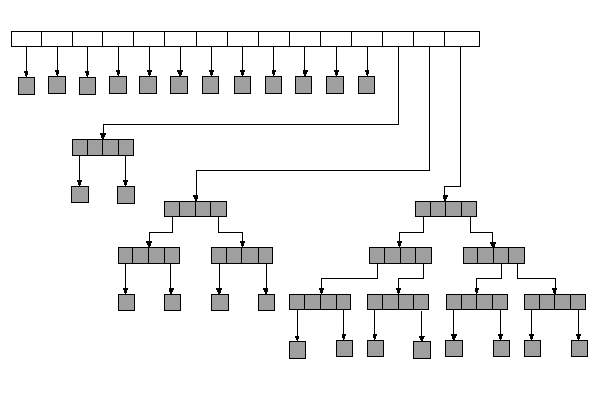
\includegraphics[width=120mm]{images/fig0419.png}
\caption{Adressering van datablokken in ext2}
\label{extAdressering}
\end{center}
\end{figure}

Het grote voordeel van deze structuur is dat de adresinformatie voor kleine bestanden volledig in het werkgeheugen
beschikbaar is. Met bestanden die maximaal 12 datablokken in beslag nemen kan dus erg snel gewerkt worden. Dat de
grootte van een bestand in ext2 beperkt is, volgt ook uit deze adresseringsstructuur. De maximale bestandsgrootte
in bytes wordt gegeven door:

\begin{displaymath}
S_{max} = \left[12 + \left(\frac{b}{4}\right) + \left(\frac{b}{4}\right)^{2} + \left(\frac{b}{4}\right)^{3}\right]b
\end{displaymath}

\TODO{FIX! Is niet helemaal juist ... max limiet is 2TB}
% http://www.nongnu.org/ext2-doc/ext2.html
% https://en.wikipedia.org/wiki/Ext2
% http://ext2read.sourceforge.net/old/ext2fs.htm


Hierin is $b$ de blokgrootte in bytes, en gaan we uit van adressen van 32 bits, dus 4 bytes per adres. Voor een
blokgrootte van 1KB geeft dit een maximale grootte van 16GB.

\subsection{Vrije blokken en inodes}

In het superblok worden tabellen bijgehouden met de adressen van een aantal vrije datablokken en een aantal vrije
inodes. In deze tabellen is echter niet voldoende plaats om alle vrije elementen te bewaren.

Wanneer b.v. een bestand moet worden uitgebreid, wordt een adres van een vrij blok uit de tabel in het superblok
genomen. Bij het verwijderen van een bestand worden de adressen van de vrijgekomen blokken in de tabel ingeschreven.
Indien de tabel leeg is op het ogenblik dat een blok aan een file moet worden toegekend zal de tabel uit het eerste
blok in de gelinkte lijst naar het superblok worden gekopieerd. Het hierdoor vrijgekomen blok wordt aan het bestand
toegevoegd. Als de tabel helemaal gevuld is met adressen, en er wordt een blok vrijgegeven, dan wordt de tabel uit
het superblok naar het vrijgekomen blok gekopieerd, waarna dit als eerste blok in de gelinkte lijst wordt opgenomen.

Voor vrije inodes wordt een gelijkaardige methode gebruikt. In het superblok staat een tabel voor 100 nummers van
vrije inodes.  Wanneer een nieuw bestand vindt men hier het nummer van een beschikbare inode. Bij het verwijderen
van een bestand wordt het nummer van de hierdoor vrijgekomen inode aan de tabel toegevoegd.

Een belangrijk verschil met de vrije blokken is de mogelijkheid om een vrije inode te herkennen aan zijn inhoud. Het
veld voor het bestandstype staat namelijk op 0 als de inode niet in gebruik is. Hierdoor moeten niet alle nummers van
vrije inodes bijgehouden worden. Wanneer de tabel in het superblok leeg is, kan de kernel de i-list doorlopen en de
nummers van de 100 eerste vrije inodes in de tabel plaatsen.

Om het zoeken naar vrije inodes zo effici\"ent mogelijk te laten verlopen, wordt de positie van de laatst gevonden
vrije inode apart bijgehouden, om de volgende zoektocht vanop die positie te kunnen starten. Wanneer er een inode
vrijkomt door het verwijderen van een bestand zijn er dan 2 mogelijkheden. Als de positie van deze inode voor de
opgeslagen positie komt wordt de opgeslagen positie erdoor vervangen. Als de positie erna komt moet er niets gebeuren,
want dan wordt de nieuwe vrije inode zowiezo gevonden bij \'e\'en van de volgende zoektochten.

\subsection{Harde en zachte links}

Omdat de bestandsbeschrijving niet in de directory bewaard wordt, kan men op een eenvoudige en effici\"ente
manier eenzelfde bestand via verschillende paden aanspreken. Men laat in dit geval 2 bestanden verwijzen
naar eenzelfde inode, en dus ook naar hetzelfde bestand. Dit wordt een \emph{hard link}\index{hard link} genoemd. Om een
acylische structuur te behouden is het niet toegelaten om hard links te cre\"eren naar directories
(zie eerder). Een hard link naar een bestand in een ander bestandssysteem kan ook niet. Voor
\emph{symbolic links}\index{symbolic link} gelden deze beperkingen niet, maar in dit geval wordt verwezen naar een ander pad,
niet naar een inode.

Het gebruik van hard links vraagt ook om een speciale aanpak bij het verwijderen. De inode en de datablokken van
een bestand mogen pas vrijgegeven worden als er geen enkele link meer is. Daarom wordt in een inode een teller
met het aantal links bijgehouden (\verb|i_nlink|). Bij symbolic links is dit niet nodig. Wanneer het bestand
waarnaar een symbolic link verwijst verwijderd wordt, blijft de link bestaan. Zo'n link wordt een wees (orphan)
genoemd.

\subsection{Bijzonderheden}

Ext2 heeft enkele specifieke eigenschappen die we nog niet tegenkwamen in andere bestandssystemen. Zo wordt
het aantal inodes in de I-list bepaald bij het aanmaken van het bestandssysteem. Een vervelend
gevolg hiervan is dat het kan gebeuren dat je geen nieuw bestand kan aanmaken, hoewel er toch nog vrije
datablokken beschikbaar zijn. Een ext2 bestandssysteem heeft dus een maximum aantal bestanden. Standaard
wordt er \'e\'en inode aangemaakt voor iedere 4096 bytes beschikbare schijfruimte. Als de gemiddelde grootte
van je bestanden kleiner is dan 4kB, kan je dus met een tekort aan inodes te maken krijgen.

Bij het cre\"eren van het bestandssysteem wordt een deel (standaard 5\%) van de blokken gereserveerd voor
de beheerder van het syteem (root). Dit voorkomt dat een gebruiker of een gebruikersproces het volledige
bestandssysteem volschrijft, waardoor het besturingssysteem zou kunnen vastlopen.

Een laatste bijzonder bestandstype is de zogenaamde \emph{device file}. Deze bestanden bevatten geen data, maar
stellen een systeemapparaat voor. Zo kan men communiceren met een apparaat door te lezen en te schrijven van of
naar de bijhorende device file. Het toetsenbord zou je dan b.v. kunnen beschouwen als een oneindig alleen-lezen
tekstbestand. Ieder getypt karakter verschijnt in het bestand. Omdat lezen per blok voor een apparaat als een
toetsenbord niet erg effici\"ent zou zijn, wordt bij device files een onderscheid gemaakt tussen karakter- en
blokapparaten.

\chapter{Procesbeheer}

Een computersysteem voert programma's uit. De gebruiker wil
programma's kunnen opstarten, tijdelijk onderbreken en afsluiten. Meerdere
programma's tegelijk uitvoeren en eventueel prioriteiten toekennen moet
ook mogelijk zijn.

\section{Processen}

Een \emph{proces}\index{proces} is niet hetzelfde als een
programma. Een proces is een programma in uitvoering. Een programma is
niet meer dan uitvoerbare code.

Wanneer zo'n programma uitgevoerd wordt moet de code in het
werkgeheugen geladen worden, maar er moet ook plaats zijn voor b.v. de
waarden van de variabelen tijdens de uitvoering.

Wanneer een programma uitgevoerd wordt omvat het proces
verschillende componenten. Er is een gereserveerd deel van het geheugen,
met daarin de uit te voeren code, maar ook de waarden van variabelen. De
processortoestand omvat de inhoud van de bevelenteller en verschillende
registers. Het besturingssysteem houdt ook gegevens bij om de uitvoering
te kunnen organiseren, zoals b.v. de bestandsbeschrijvingen van
bestanden die door het proces geopend zijn of de eigenaar en de
toegangsrechten van het proces.

Eenzelfde programma kan tegelijkertijd door verschillende
processen uitgevoerd worden, zoals de schermafdruk illustreert. Dan moet
voor iedere uitvoering een apart deel van het geheugen beschikbaar zijn
om de toestand van het proces bij te houden.

\subsection{Multiprogrammatie}

Een processor kan maar \'e\'en programma tegelijkertijd uitvoeren.
Als we toch meerdere processen willen uitvoeren is de meest voor de
hand liggende oplossing meerdere processoren gebruiken. Maar als het
aantal gelijktijdige processen groeit, stijgt ook het aantal
processoren dat we nodig hebben. Dit is natuurlijk een te dure
oplossing voor een eenvoudig computersysteem. Bovendien zullen een
aantal van de processoren stilstaan als niet het maximum aantal
gelijktijdige processen beschikbaar is voor uitvoering.

Als we op een uniprocessor-systeem op hetzelfde ogenblik
meerdere processen willen uitvoeren, moeten we het
\emph{multiprogrammatie}\index{multiprogrammatie} principe toepassen. De
rekentijd op \'e\'en processor wordt dan verdeeld over meerdere processen.
De processen kunnen om beurt voor een bepaalde tijd gebruik maken van
de processor.

Het kan gaan om verschillende processen van dezelfde gebruiker.
Als we verschillende gebruikers tegelijkertijd op \'e\'en processor laten
werken door hun processen via multiprogrammatie uit te voeren spreken
we van \emph{timesharing}\index{time sharing}. Het lijkt alsof
verschillende processen tegelijkertijd verwerkt worden, maar in
werkelijkheid wisselt de processor van het ene proces naar het andere.
Het is het besturingssysteem dat de uitvoering van meerdere processen
gaat verweven om het processorgebruik te maximaliseren en tegelijk te
zorgen voor een aanvaardbare responstijd. Het onderdeel van het
besturingssysteem dat deze taak verzorgt heet de
\emph{scheduler}\index{scheduler}.

\begin{figure}
\centering
\begin{subfigure}{.5\textwidth}
  \centering
  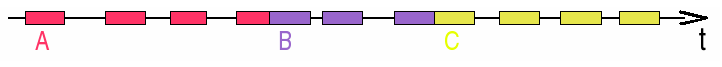
\includegraphics[width=100mm]{images/fig0501a.png}
  \caption{Zonder multiprogrammatie}
  \label{multprogr:a}
\end{subfigure}%
\begin{subfigure}{.5\textwidth}
  \centering
  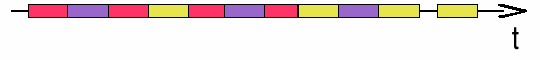
\includegraphics[width=75mm]{images/fig0501b.png}
  \caption{Met multiprogrammatie}
  \label{multprogr:b}
\end{subfigure}
\caption{Multiprogrammatie}
\label{multprogr}
\end{figure}

Als we geen gebruik maken van multiprogrammatie worden de
verschillende processen na mekaar uitgevoerd. Wanneer het proces in
uitvoering moet wachten op een externe gebeurtenis, zoals b.v. het
afwerken van een leesopdracht door een schijf of het resultaat van een
ander proces, staat de processor stil.

Door multiprogrammatie toe te passen kunnen we het
processorgebruik verbeteren. Als \'e\'en proces wacht op een gebeurtenis
kan de processor een ander proces uitvoeren.

In fig. \ref{multprogr} zien we duidelijk dat de processor bijna niet
meer werkloos is, alleen op het einde wanneer processen A en B
voltooid zijn is er geen ander proces beschikbaar om uit te voeren
terwijl C wacht. Merk op dat proces A eigenlijk nadeel ondervindt van
de multiprogrammatie, aangezien het nu later voltooid zal zijn.

Naast het optimaliseren van het processorgebruik zorgt
multiprogrammatie ook voor een lagere gemiddelde responstijd. De
\emph{responstijd} is de tijd tussen het geven van een
opdracht en het moment dat de ontvangst van het antwoord begint. Dit
is van belang bij interactief werken met een systeem. Bij timesharing
is het dus van belang om de responstijd zo laag mogelijk voor alle
gebruikers die het systeem delen.

Zoals we multiprogrammatie nu voorstellen blijven we een proces
uitvoeren tot het proces op een gebeurtenis wacht. Een proces dat zeer
veel rekenwerk moet doen, en weinig invoer- of uitvoeropdrachten bevat
waarop gewacht moet worden kan de processor dan relatief lang bezet
houden. Dit is slecht voor de gemiddelde responstijd omdat alle andere
processen dan zolang moeten wachten. Daarom zal het besturingssysteem
een proces soms na een bepaalde tijd onderbreken om andere processen
uit te kunnen voeren. Dit onderbreken noemen we
\emph{preemption}\index{preemption}.

\subsection{Toestanden van een proces}

Tijdens zijn uitvoering doorloopt een proces een aantal
toestanden. De overgangen tussen deze verschillende toestanden worden
teweeggebracht door de werking van het uitgevoerde programma ofwel
door de scheduler.

In het eenvoudigste geval zijn er twee toestanden: actief en
niet-actief. Een proces is actief als het uitgevoerd wordt door de
processor.

\begin{figure}
\begin{center}
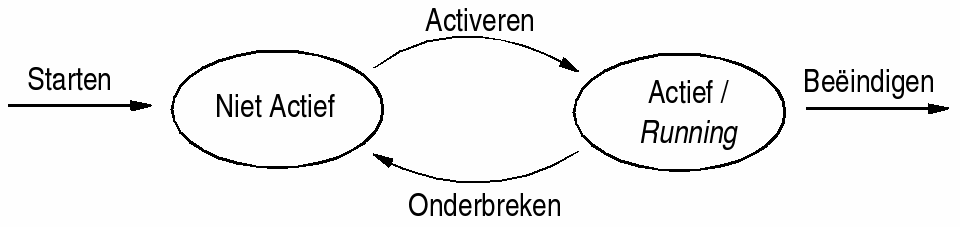
\includegraphics[width=100mm]{images/fig0502.png}
\caption{Twee toestanden van een proces}
\label{toestproc1}
\end{center}
\end{figure}

Wanneer een proces gestart wordt, zal het klaargemaakt worden
voor uitvoering en komt het in een niet-actieve toestand. De scheduler
zal dan een proces om uit te voeren kiezen uit alle niet-actieve
processen. Dit proces wordt dan actief. Wanneer het actieve proces
onderbroken wordt, en dus niet-actief wordt zal een ander proces
gekozen worden om uitgevoerd te worden.

Een proces wordt be\"eindigd als alle code is uitgevoerd. Omdat de
processor de code uitvoert kan een proces enkel aflopen vanuit de
actieve toestand. Wanneer het proces niet-actief is wacht het om
uitgevoerd te worden, en kan het dus nog niet be\"eindigd zijn.

Zoals reeds besproken zijn er 2 soorten onderbrekingen mogelijk
voor een proces in uitvoering. Enerzijds kan het proces door het
aanvragen van een invoer- of uitvoeropdracht moeten wachten. Dan wordt
het niet-actief. Anderzijds is er preemption, waarbij de scheduler het
actieve proces onderbreekt om een ander proces te kunnen starten. De
niet-actieve toestand moet dus opgesplitst worden in 2 aparte
toestanden: een geblokkeerd proces wacht op in- of uitvoer, en de
processen die gereed zijn kunnen door de scheduler gekozen worden om
uitgevoerd te worden.

\begin{figure}
\begin{center}
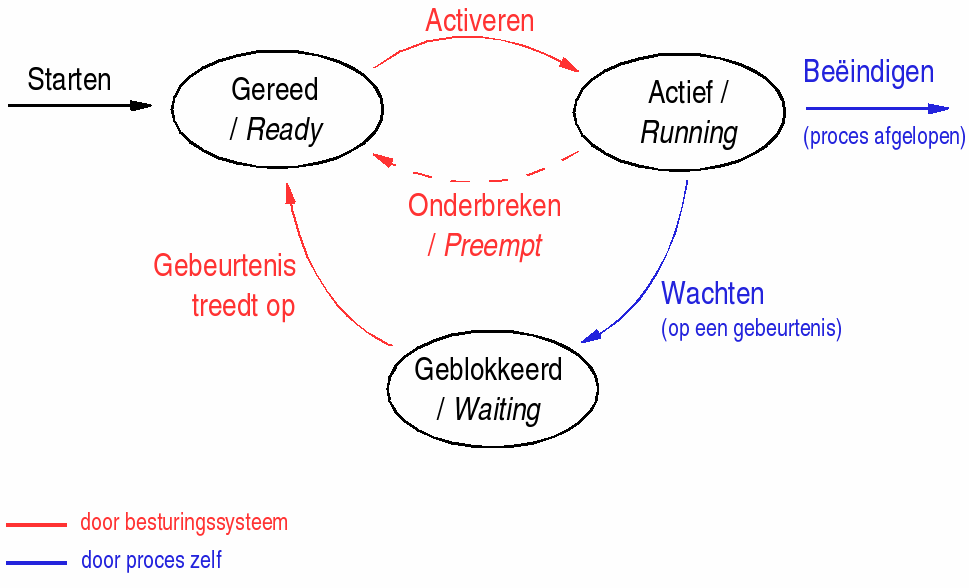
\includegraphics[width=100mm]{images/fig0503.png}
\caption{Drie toestanden van een proces}
\label{toestproc2}
\end{center}
\end{figure}


Processen die 'gereed' zijn, worden door het besturingssysteem
in een wachtrij bijgehouden. De scheduler kan uit deze wachtrij \'e\'en
proces activeren. Dit proces wordt dan actief en wordt door de
processor uitgevoerd. Er zijn drie manieren waarop een proces de
actieve toestand kan verlaten. Wanneer het proces afgelopen is zal het
natuurlijk niet langer actief zijn. Als het proces via een system call
een aanvraag doet waarvan het resultaat niet onmiddellijk beschikbaar
is zal het 'geblokkeerd' worden. Dit gebeurt dus op initiatief van het
proces zelf. Tenslotte kan ook het besturingssysteem een actief proces
onderbreken en terug aan de wachtrij toevoegen d.m.v. preemption. Dit
mechanisme is niet in alle systemen beschikbaar. Er zijn preemptive en
non-preemptive schedulers.

Processen die vaak in- en uitvoer nodig hebben, en dus vaak
'geblokkeerd' zijn, noemen we \emph{I/O-gebonden
processen}\index{I/O-gebonden processen}. Processen die veel rekenwerk doen en zelden op
externe gebeurtenissen wachten noemen we verwerkingsgebonden of
\emph{CPU-gebonden} processen.\index{CPU-gebonden processen}

\TODO{5-toestandsdiagram van een proces?}

\section{Scheduling}

Het is nu duidelijk dat de belangrijkste taak van de scheduler is
om te beslissen welk proces uitgevoerd zal worden. De bedoeling van deze
component van het besturingssysteem is om het computersysteem, en
meerbepaald de processor, zo goed en effici\"ent mogelijk te gebruiken. De
eerste vraag die zich stelt is hoe we deze kwaliteit en effici\"entie
moeten meten zodat we verschillende strategie\"en kunnen vergelijken. We
proberen effici\"entie daarom te vertalen in een aantal concrete
doelstellingen:

\begin{description}
\item[Rechtvaardigheid] Alle processen dienen op een rechtvaardige wijze te
worden behandeld. Geen enkel proces mag blijvend achteruit gesteld worden,
waardoor de uitvoering ervan onmogelijk zou worden.
\item[Doorvoer maximaliseren] De \emph{doorvoer}
(\emph{throughput})\index{throughput} is de hoeveelheid werk die per tijdseenheid
wordt gepresteerd (b.v. het aantaljobs dat per uur wordt afgewerkt).
\item[Omlooptijd minimaliseren] De \emph{omlooptijd}
(\emph{turnaround time})\index{turnaround time} is de tijd die verloopt tussen het
indienen van een proces en het voltooien ervan en wordt bekomen als een som van
wachttijden en de werkelijke uitvoeringstijd. In andere woorden, de omplooptijd
is de het verschil tussen het tijdstip waarop het proces voltooid is en het
tijdstip waarop het proces gestart wordt. Deze maat is vooral geschikt voor
batch-taken.
\item[Responstijd minimaliseren] De responstijd (response time)\index{response time} is de tijd die
verloopt tussen het ingeven van een bevel en het moment waarop de ontvangst van
het antwoord begint. Deze grootheid speelt vooral een rol bij interactief
werken, omdat een gebruiker dan niet al te lang op een reactie van het systeem
wil wachten.
\item[Voorspelbaarheid] De werking van het systeem moet voorspelbaar zijn. Zo
mogen doorvoer, omlooptijd en responstijd niet te sterk veranderen in de tijd,
bijvoorbeeld onder invloed van een wisselende belasting van het systeem.
\item[Overhead beperken] De processortijd die het besturingssysteem zelf
gebruikt voor berekeningen of om processen te wisselen kan ook niet gebruikt
worden om de processen van de gebruikers uit te voeren. Deze overhead moet
binnen redelijke grenzen blijven.
\end{description}

Het is duidelijk dat niet ieder van deze doelstellingen even
gemakkelijk te meten is. De doelstellingen met de prestaties van het
systeem te maken hebben, zoals bij responstijd of omlooptijd, zijn het
best te meten. Doelstellingen als voorspelbaarheid en rechtvaardigheid
laten zich niet zo gemakkelijk in getallen vatten.

Er is ook een onderscheid tussen gebruikersgerichte en
systeemgerichte doelstellingen. Zo be\"invloeden de respons- en omlooptijd
rechtstreeks de ervaring van de gebruiker met het systeem. De doorvoer
daarentegen geeft aan hoe effici\"ent het systeem werkt, vandaar dat het
een geschikte maat is voor batchverwerking.

\section{Niet-pre\"emptieve Scheduling-strategie\"en}

Bij deze eerste strategie\"en heeft de scheduler niet de
mogelijkheid een proces te onderbreken. Eens een proces uitgevoerd wordt
kan alleen het proces zelf de processor terug vrijgeven, hetzij doordat
het zichzelf blokkeert om te wachten op een gebeurtenis, of omdat het
proces zichzelf be\"eindigt. Er is dus geen overgang van 'actief' naar
'gereed'.

Het ontbreken van de mogelijkheid tot onderbreken zorgt ervoor dat
de scheduler slechts een beperkte invloed heeft, en b.v. heel moeilijk
voor voorspelbaarheid of een lage responstijd kan zorgen.

\subsection{First Come First Served (FCFS)}

Dit algoritme\index{first come first served} gaat de processen verwerken in dezelfde volgorde
waarin ze in de wachtrij werden geplaatst. We noemen zo'n wachtrij ook
een First In First Out of FIFO wachtrij. De scheduler moet enkel het
eerste element uit de FIFO-rij nemen. Je kan het vergelijken met een
rij mensen die aanschuift aan een loket.

Dit is een erg eenvoudig algoritme, en het lijkt natuurlijk erg
rechtvaardig. Om dit na te gaan bekijken we een situatie met 4 processen. Het
moment waarop de processen in de wachtrij aankomen, en hun uitvoeringstijden
($T_u$) zijn gekend. We berekenen dan de omlooptijd ($T_o$).

\begin{center}
\begin{tabular}{|l|r|r|r|r|r|r|}
\hline
Proces & Aankomst & $T_u$ & Start & $T_o$ & ${T_o}$/${T_u}$ \\
\hline
A & 0 &   1 &   0 &   1 &    1 \\
B & 1 & 100 &   1 & 100 &    1 \\
C & 2 &   1 & 101 & 100 &  100 \\
D & 3 & 100 & 102 & 199 & 1,99 \\
\hline
\end{tabular}
\end{center}

Om de resultaten gemakkelijker te interpreteren berekenen we ook de
genormaliseerde omlooptijd. De \emph{genormaliseerde omlooptijd}\index{genormaliseerde omlooptijd} bekom
je door de omlooptijd te delen door de uitvoeringstijd. Het is een maat
voor de relatieve vertraging die een proces ondervindt. Het proces
werd niet vertraagd als $\frac{T_o}{T_u} = 1$. Hoe hoger $\frac{T_o}{T_u}$, hoe
slechter het proces werd bediend. De genormaliseerde omlooptijd brengt houdt
rekening met het feit dat een bijkomende wachttijd van 10 ms een grotere
nadelige
invloed heeft op een proces met een korte uitvoeringstijd dan op een proces met
een langere uitvoeringstijd. Een half uur in de file staan is minder vervelend
tijdens een verplaatsing over een lange afstand dan bij een korte trip van een
kwartier\footnote{Het gaat hier om het nadelige effect van de tijd in de file
op de totale duur van de verplaatsing. We meten niet hoe hard je vloekt op het
moment dat je in de file terechtkomt...}.

Proces C is hiervan een extreem voorbeeld. Meestal geldt ook: hoe
langer de uitvoeringstijd van een proces, hoe groter de absolute
vertraging die men kan tolereren. Vergelijk daartoe proces D met C. D
heeft even lang moeten wachten om te beginnen maar
$\frac{T_u}{T_t}$ is veel lager en acceptabel. Men kan besluiten dat FCFS
meestal gunstiger is voor lange processen.

Hierdoor is FCFS ook voordelig voor verwerkingsgebonden
processen, omdat I/O-gebonden processen de processor zelf vlugger
vrijgeven en dan weer achteraan de FIFO-rij moeten gaan staan.

\subsection{Shortest Job First (SJF)}

De bevoordeling van langere processen door FCFS kan verminderd
worden door telkens dat proces te kiezen dat het minst lang actief zal
zijn, m.a.w. het kortste proces. Deze strategie\index{shortest job first} kan wel leiden tot
\emph{starvation}\index{starvation}: langere processen
\emph{verhongeren} zolang er een aanvoer is van
kortere processen.

Algemeen zal deze strategie een lagere gemiddelde omlooptijd
opleveren. De omlooptijd zal altijd bestaan uit de eigenlijke
uitvoeringstijd, verhoogd met eventuele wachttijden. Wanneer twee
processen na mekaar uitgevoerd worden, dan zal voor het tweede proces
de omlooptijd bestaan uit een wachttijd gelijk aan de uitvoeringtijd
van het eerste proces, en de eigen uitvoeringstijd. Voor het eerste
proces is de omlooptijd uiteraard gelijk aan de uitvoeringstijd. De
enige wachttijd bestaat dus uit de uitvoeringstijd van het eerst
uitgevoerde proces.

De volgorde, waarin de twee processen aan bod komen, bepaalt nu
de grootte van de wachttijd. De kleinste gemiddelde omlooptijd zal
worden verkregen indien eerst het proces met de kleinste
uitvoeringstijd aan bod komt. Zo wordt immers het enige veranderlijke
element, de wachttijd voor het tweede proces, minimaal.

De grootste moeilijkheid bij deze methode is echter dat de
uitvoeringstijd moet gekend zijn, wat eigenlijk een element is uit de
toekomst. Bij processor scheduling kan men alleen het gedrag van het
betrokken proces in het verleden nagaan en hieruit een prognose
afleiden voor de toekomstige uitvoerperiodes. Merk op dat we het hier
niet hebben over de totale uitvoeringstijd van een proces, maar over
de tijd tot het proces de volgende keer geblokkeerd wordt.

Stel dat $t_i$ de uitvoeringstijd is van uitvoeringsperiode $i$, en
$T_i$ een voorspelling voor uitvoeringsperiode $i$. De eenvoudigste
voorspelling is een gemiddelde van de duur van de vorige
uitvoeringstijden:

\begin{displaymath}
T_{n+1} = \frac{\sum_{i=1}^{n}t_i}{n} = \frac{t_1 + t_2 + \ldots + t_n}{n}
\end{displaymath}

Om niet telkens het gemiddelde van alle vorige
uitvoeringsperiodes te moeten berekenen kunnen we de vorige schatting
gebruiken, waarvoor we al een berekening gemaakt hadden. We krijgen
dan:

\begin{displaymath}
T_{n+1} = \frac{t_n}{n} + \frac{n-1}{n}T_n
\end{displaymath}

Dit komt overeen met een een opeenvolging van
schattingen:

%\begin{displaymath}
\begin{eqnarray*}
T_2 & = & \frac{t_1}{1} + \frac{0}{1}T_1 = t_1 \\
T_3 & = & \frac{t_2}{2} + \frac{1}{2}T_2       \\
T_4 & = & \frac{t_3}{3} + \frac{2}{3}T_3
\end{eqnarray*}
%\end{displaymath}

Om te zien dat dit eigenlijk opnieuw het gemiddelde is van de
vorige uitvoeringsperioden werken we de formule uit voor b.v.
T4:

\begin{eqnarray*}
T_4 & = & \frac{t_3}{3} + \frac{2}{3}T_3 \\
    & = & \frac{t_3}{3} + \frac{2}{3}\Bigg(\frac{t_2}{2} + \frac{1}{2}T_2\Bigg)
\\
    & = & \frac{t_3}{3} + \frac{2}{3}\frac{t_2}{2} + \frac{2}{3}\frac{1}{2}T_2
\\
    & = & \frac{t_3}{3} + \frac{t_2}{3} + \frac{1}{3}T_2 \\
    & = & \frac{t_3}{3} + \frac{t_2}{3} + \frac{1}{3}t_1 \\
T_4 & = & \frac{t_1 + t_2 + t_3}{3}
\end{eqnarray*}

Meestal wordt ervoor gezorgd dat de tijd van meer recente
uitvoeringsperioden een grotere invloed heeft op de schatting dan die
van oudere uitvoeringsperioden. Dit kan je bekomen door een
exponentieel gewogen gemiddelde te berekenen. Met a als gewichtsfactor
tussen 0 en 1 krijgen we de volgende recursieve formule:

\begin{displaymath}
T_{n+1} = at_n + (1-a)T_n
\end{displaymath}


We bekomen dus weer een opeenvolging van schattingen:

\begin{eqnarray*}
T_2 & = & at_1 + (1-a)T_1 \\
T_3 & = & at_2 + (1-a)T_2 \\
T_4 & = & at_3 + (1-a)T_3
\end{eqnarray*}

Als we T4 weer als voorbeeld nemen krijgen we:

\begin{eqnarray*}
T_4 & = & at_3 + (1-a)T_3 \\
    & = & at_3 + (1-a)\Big(at_2 + (1-a)T_2\Big) \\
    & = & at_3 + (1-a)at_2 + (1-a)^2T_2 \\
    & = & at_3 + (1-a)at_2 + (1-a)^2\Big(at_1 + (1-a)T_1\Big) \\
    & = & at_3 + (1-a)at_2 + (1-a)^2at_1 + (1-a)^3T_1
\end{eqnarray*}


Als a tussen $0$ en $1$ ligt, dan geldt dat ook voor $(1-a)$. Een
oudere uitvoeringsperiode wordt vermenigvuldigd met een steeds hogere
macht van $(1-a)$, dus het belang van deze factor neemt steeds
af.

Voor $a=0,5$ krijgen we voor $T_4$ bijvoorbeeld:

\begin{displaymath}
T_4 = \frac{1}{2}t_3 + \frac{1}{4}t_2 + \frac{1}{8}t_1 + \frac{1}{8}T_1
\end{displaymath}


\subsection{Priority Scheduling}

In dit algoritme wordt met elk proces een prioriteit $p$
verbonden. We selecteren dan telkens het proces met de hoogste
prioriteit (veelal, maar niet altijd, aangeduid door de grootste
waarde van $p$). Het vorige algoritme, SJF, is eigenlijk een voorbeeld
van priority scheduling\index{priority scheduling}. Voor een proces dat een hoeveelheid T processortijd
nodig heeft neemt men dan $p = \frac{1}{T}$ als waarde voor de prioriteit.
Prioriteiten kunnen intern bepaald zijn, d.w.z. afgeleid van een eigenschap van
het betrokken proces, zoals het gebruik van hulpbronnen, de geschatte
uitvoeringstijd of het al dan niet verwerkingsgebonden karakter. Externe
prioriteiten worden van buitenaf opgelegd, b.v. naar gelang de herkomst van het
proces. Processen van docenten zouden een hogere prioriteit kunnen krijgen dan
processen van studenten.

Een probleem bij priority scheduling is terug het verhongeren
van een proces. De mogelijkheid bestaat dat een proces met de
laagste prioriteit voortdurend wordt voorafgegaan door nieuwe
processen met een hogere prioriteit, en zo nooit aan de beurt komt. Om dit te
voorkomen wordt meestal een systeem van \emph{veroudering} (\emph{aging}\index{aging})
ingevoerd. Dit betekent dat de prioriteit van een proces stijgt naarmate het
proces langer in de wachtrij zit. De scheduler zou b.v. bij elke tussenkomst de
prioriteit van alle processen in de wachtrij met 1 kunnen verhogen (tot een
maximale waarde). Op die manier zal uiteindelijk elk proces binnen een redelijke
termijn aan bod komen.

\section{Pre\"emptieve Scheduling-strategie\"en}

\TODO{aanvullen}

\subsection{Round Robin}

\TODO{aanvullen}

\subsection{Shortest Remaining Time}

\TODO{aanvullen}

\subsection{Priority Scheduling}

\TODO{aanvullen}

\section{Voorbeeld: de Windows scheduler}

\TODO{aanvullen}

Numa cores
Energiebeheer
Variabele klokfrequentie

%%\chapter{Threads}

\section{Multithreading modellen}

\section{Problemen}

\section{Synchronisatie}

\subsection{Kritische secties}

\subsection{Semaforen}

\subsection{Monitoren}

\subsection{Deadlock}

\chapter{Geheugenbeheer}

Een van de belangrijkste taken die het besturingssysteem heeft, is het beheer
van het werkgeheugen. Het besturingssysteem moet kiezen waar de programma's in
het geheugen terecht komen, hoeveel geheugen elk programma toegewezen krijgt,
welke stukken code aan welke stukken geheugen mogen komen, enz. Er zijn
verschillende strategie\"en mogelijk om het geheugen te beheren, elk met zijn
voor- en nadelen.

\section{Segmentatie}

In het vak Computersystemen werd er al een vorm van geheugenbeheer besproken:
\emph{segmentatie}. Een programma wordt hierbij in verschillende stukken
gebroken --- \emph{segmenten} --- die elk logisch bij elkaar horen. Zo kan er bijvoorbeeld een
codesegment zijn waar alle instructies van het programma in staan. Het
datasegment bevat dan weer de data van de applicatie, en het stapelsegment bevat
de data die het programma op de stapel opslaagt. De Intel x86-processor biedt
ondersteuning voor een maximum van zes segmenten per programma.

Elk segment heeft een beginpunt (de \emph{basis}) en een bepaalde grootte. Het
besturingssysteem kiest bij het inladen van het programma waar elk segment
terecht komt in het werkgeheugen. Aangezien segmenten geen vaste plaats in het geheugen hebben, kan
een programma dus geen gebruik maken van absolute adressering (d.w.z. het
gebruik van de fysische adressen zoals ze door het RAM-geheugen gebruikt
worden). In de plaats daarvan wordt relatieve adressering gebruikt, waarbij een
programma altijd werkt met een \emph{verplaatsing} binnen een segment.

Om segmentatie effici\"ent te laten werken, is ondersteuning van de hardware
vereist. In het geval van de Intel x86-processor vertaalt zich dat naar de
volgende componenten:

\begin{itemize}
\item{\textbf{Descriptor}} Een descriptor is een gegevensstructuur die
een segment beschrijft. Het bevat onder andere het beginadres van het segment en
de lengte van het segment.
\item{\textbf{Descriptorentabel}} Er kunnen meerdere
programma's tegelijkertijd in het geheugen geladen zijn, en elk programma kan
meerdere segmenten hebben. Al de descriptoren die bij deze segmenten horen,
staan opgeslagen in de descriptorentabel. Deze tabel staat ergens in het
werkgeheugen opgeslagen en kan maximaal 8192 descriptoren bevatten.
\item{\textbf{Segmentselector}} Om een bepaalde descriptor uit de descriptorentabel aan
te duiden, kunnen we een getal gebruiken dat het volgnummer van de descriptor in
de tabel voorstelt. Dit getal noemen we een segmentselector.
\item{\textbf{Segmentregister}} De processor voorziet zes registers die tijdens de
uitvoering van een programma kunnen gebruikt worden om informatie over de
segmenten op te zoeken. Deze registers bevatten segmentselectors, waarmee de
processor dan naar de descriptorentabel kan gaan om de informatie van het
segment uit te lezen.
\end{itemize}

Wanneer een besturingssysteem een proces selecteert om uit te voeren, zullen de
segmentregisters ge\"initialiseerd worden met de correcte segmentselectors die
bij het programma horen. Bijvoorbeeld, in segmentregister \texttt{ds} komt de segmentselector
van de descriptor die het datasegment van de applicatie beschrijft.

Wanneer een applicatie een een instructie oproept die het geheugen aanspreekt, zal de instructie telkens de gewenste verplaatsing \'en het gewenste segment bevatten. Bijvoorbeeld, de instructie \texttt{mov al, [ds:1234]} haalt de byte op uit het geheugen die staat in het datasegment op verplaatsing 1234. Bij de uitvoering van deze instructie zal de processor een adresberekening doen. Eerst wordt door middel van de segmentselector in segmentregister \texttt{ds} de gevraagde descriptor opgehaald uit de descriptorentabel. De verplaatsing wordt vergeleken met de grootte van het segment; indien de gevraagde verplaatsing groter is zal de processor een fout genereren. Uiteindelijk zal bij de verplaatsing de basis opgeteld worden, om zo het fysieke adres te krijgen dat uit het werkgeheugen moet opgehaald worden. Figuur~\ref{segmentatie} geeft dit schematisch weer.

\begin{figure}
\begin{center}
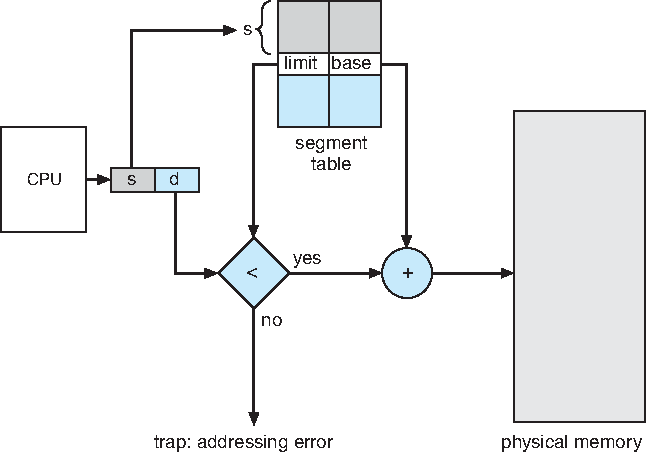
\includegraphics[width=100mm]{images/segmentatie.pdf}
\end{center}
\caption{Adresberekening bij segmentatie}
\label{segmentatie}
\end{figure}

Segmentatie heeft een aantal belangrijke voordelen. Zo kan een programma een groter stuk geheugen aanspreken dan dat de woordgrootte van de processor toelaat. Bijvoorbeeld, op een 16-bit processor bestaat een verplaatsing uit 16 bits. Dit wil zeggen dat de maximum grootte van een segment 2\textsuperscript{16} of 65536 bytes is. Wanneer er meer geheugen beschikbaar is, dan kan de applicatie gebruik maken van meerdere segmenten die elk een ander stuk fysisch geheugen beslaan.

De verschillende segmenten van een programma kunnen ook andere toegangsrechten krijgen. Zo kan het codesegment bijvoorbeeld allen-lezen gemaakt worden, en het datasegment niet-uitvoerbaar. Dit is van belang om er voor te zorgen dat bepaalde softwarefouten niet uitgebuit kunnen worden door een aanvaller.

Aangezien er enkel met verplaatsingen gewerkt wordt, is het programma verplaatsbaar in het geheugen. Elke keer dat het programma opgestart wordt, kan het ergens anders in het geheugen ingeladen worden. Ook kan hetzelfde programma meerdere keren in het geheugen staan. Deze eigenschap zorgt er voor dat het geheugenbeheer een stuk geavanceerder kan verlopen. Zo kan het besturingssysteem bij het inladen van het programma de meest-optimale plaats in het geheugen voor het programma zoeken. Wanneer een programma twee keer gestart wordt, kan het besturingssysteem er ook voor kiezen om bijvoorbeeld het codesegment te delen.

Het grootste nadeel van segmentatie heeft te maken met \emph{externe fragmentatie}. Net zoals bij het beheer van aaneengesloten bestanden, kunnen er bij segmentatie gaten vallen in het geheugen. Wanneer een klein segment verwijderd wordt, kan het stuk vrij geheugen te klein zijn om er een nieuw (groter) segment in te steken. Naarmate de tijd vordert, kan dit oplopen tot een aanzienlijk stuk van het geheugen dat niet meer gebruikt kan worden.

Een tweede nadeel is dat de segmenten van een programma altijd in hun geheel moeten worden ingeladen in het geheugen, ook al wordt er slechts een deel van het segment daadwerkelijk actief gebruikt.

\section{Paginatie}

Een manier om de twee nadelen van segmentatie op te lossen, is door te werken met \emph{pagina's} in plaats van segmenten. Een pagina is een stuk geheugen met een vaste grootte (bijv. 4KB). Een programma kan dan opgedeeld worden in meerdere pagina's. Het werkgeheugen wordt op een gelijkaardige manier opgedeeld in \emph{frames}; dit zijn blokken die dezelfde grootte hebben als een pagina. Wanneer een programma dan in het geheugen geladen wordt, moet het besturingssysteem de pagina's van het proces inladen in frames van het werkgeheugen die nog vrij zijn. De volgorde van de pagina's in een proces en de frames in het werkgeheugen staat volledig los van elkaar. Zo moeten opeenvolgende pagina's van een proces niet per se in opeenvolgende frames van het werkgeheugen gestoken worden.

Per proces maakt het besturingssysteem ook een \emph{paginatabel} (of \emph{page table}) aan. In deze tabel wordt de mapping tussen de pagina's van het proces en de frames van het werkgeheugen bijgehouden. Aangezien elk proces een andere paginatabel heeft, moet de CPU weten welke tabel hij wanneer moet gebruiken. De processor maakt hier een speciaal register voor beschikbaar, dat door het besturingssysteem beheerd wordt. Dit register wijst te allen tijde naar het adres van de actieve paginatabel. Wanneer het besturingssysteem een nieuw proces actief maakt, moet het dus de waarde in dit register aanpassen.

Figuur~\ref{pages-frames} geeft een voorbeeld van hoe de pagina's van een programma door middel van een page table gemapped kunnen worden op de frames van het werkgeheugen.

\begin{figure}
\begin{center}
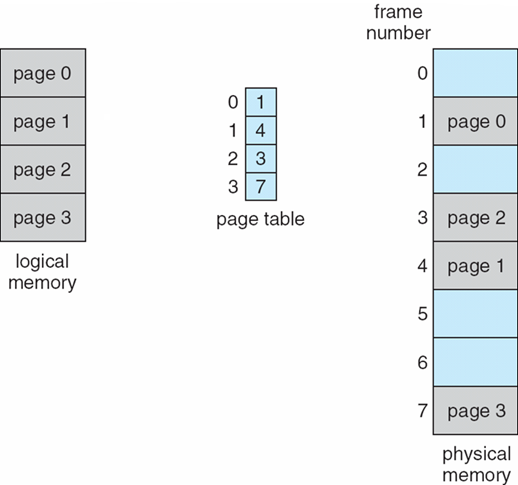
\includegraphics[width=100mm]{images/pages_frames.png}
\end{center}
\caption{De mapping van pagina's op frames}
\label{pages-frames}
\end{figure}

Paginatie vermijdt externe fragmentatie omdat de frames die vrij komen steeds kunnen worden hergebruikt voor pagina's van nieuwe processen. Dit komt omdat de pagina's van alle processen steeds dezelfde grootte hebben. Omdat een proces opgedeeld moet worden in blokken, kan er zich echter wel \emph{interne fragmentatie} voordoen. Dit is het geheugen dat verloren gaat omdat een programma soms niet exact past in een bepaald aantal blokken. In dat geval zullen een aantal bytes van het laatste blok niet gebruikt worden. Gemiddeld gezien verliezen we een halve blok per programma aan deze interne fragmentatie. Programma's hoeven ook niet meer in hun geheel ingeladen te worden. Enkel de pagina's die nodig zijn moeten in het werkgeheugen te staan.

Wanneer een programma een adres gebruikt, wordt dat opgesplitst in twee delen: een \emph{paginanummer} en een \emph{offset}. Stel dat we werken met 32-bit adressen en pagina's van 4KB. Om elke byte van een 4KB-pagina te kunnen adresseren, zal de offset moeten bestaan uit 12 bits ($2^{12} = 4096$). De resterende 20 bits van het adres stellen dus het paginanummer voor, wat betekent dat er in ons voorbeeld maximaal $2^{20} = 1048576$ pagina's zijn. De overeenkomstige adresberekening wordt weergegeven in Figuur~\ref{paging}. Aangezien deze adressen ge\"interpreteerd moeten worden en dus niet rechtstreeks overeenkomen met een adres in het werkgeheugen, noemen we ze \emph{virtuele adressen}.

\begin{figure}
\begin{center}
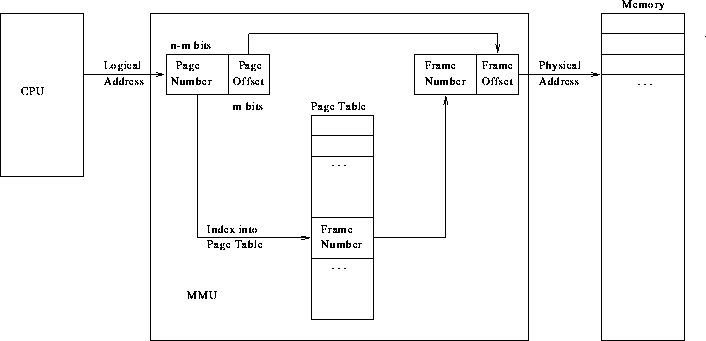
\includegraphics[width=110mm]{images/paging_hardware.png}
\end{center}
\caption{Adresberekening bij paging}
\label{paging}
\end{figure}

\subsection{Two-level page table}

Als we met hetzelfde voorbeeld van een computer met 32-bit adressen en 4KB pagina's verder gaan, dan kunnen we berekenen hoe groot een page table wordt. In een page table moet voor elk frame in het geheugen een \emph{page table entry} bijgehouden worden. Aangezien er $2^{20}$ frames zijn, moeten er dus evenveel entries beschikbaar zijn. Op de x86-processor is een page table entry 4 bytes groot, dus dan kunnen we berekenen dat een volledige page table 4MB groot is. Merk op dat elk proces een aparte page table heeft, en er dus voor elk proces 4MB geheugen gealloceerd moet worden, ook al gebruikt het proces slechts een klein stuk geheugen.

Om page tables effici\"enter in het geheugen op te slaan, kunnen we gebruik maken van een \emph{two-level page table}. Er wordt dan gebruik gemaakt van een hi\"erarchische structuur zoals beschreven in Figuur~\ref{paging-x86} waarbij een \emph{page directory} links bevat naar verschillende (kleinere) page tables. Niet elke link van de page directory moet in gebruik zijn; indien het programma weinig geheugen gebruikt, is \'e\'en link misschien al voldoende. Per proces is er slechts \'e\'en page directory. De processor weet waar die tabel in het geheugen staat, omdat het besturingssysteem het adres ervan in een speciaal register zet (op de Intel x86-processoren heet dit register \emph{control register 3} of kortweg \texttt{CR3}).

In dit geval wordt het 32-bit adres opgesplitst in 3 stukken: 12 bits voor de offset binnen de pagina, 10 bits die het paginanummer voorstellen en 10 bits die de index binnen de page directory voorstellen. Hieruit kunnen we afleiden dat in een page table en de page directory slechts $2^{10} = 1024$ entries kunnen.

\begin{figure}
\begin{center}
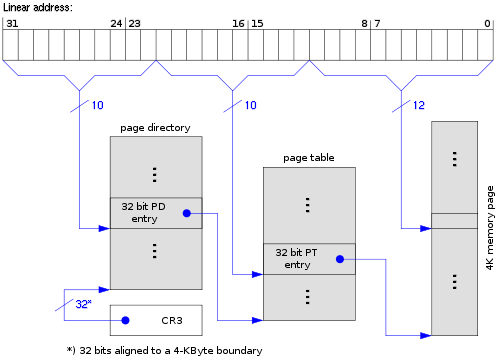
\includegraphics[width=110mm]{images/x86-paging.png}
\end{center}
\caption{Paging op de Intel x86-processor.}
\label{paging-x86}
\end{figure}

Een programma dat heel veel geheugen gebruikt, zal elke entry in de page directory gebruiken. Er zullen dus 1024 page tables gebruikt worden die elk 4KB groot zijn (= 4 bytes * 1024 entries per page table). Wat het geheugengebruik betreft is in dit geval de grootte van de two-level page table vergelijkbaar met de grootte van het vorige systeem waar er slechts \'e\'en page table per proces was.

Het voordeel van de two-level page table is pas te zien wanneer de applicatie weinig geheugen gebruikt. In dit geval gebruikt de applicatie slechts \'e\'en kleine page table, wat neerkomt op een geheugengebruik van 8KB (= 4KB voor de page table en 4KB voor de page directory). Dat is aanzienlijk minder dan de 4MB die nodig zou zijn zonder een two-level page table.

\subsection{Multi-level page table}\label{multi-level-page-table}

Een two-level page table werkt goed voor een processor met een 32-bits geheugenruimte, maar het systeem schaalt niet zo goed naar 64 bits. Stel dat we een two-level page table willen toepassen op een 64-bit processor en dat we pagina's van 4KB gebruiken. Van de 64 bits in een adres, worden 12 bits gebruikt voor de offset binnen in een pagina. De resterende 52 bits kunnen dan opgesplitst worden voor de offset van de page directory en het paginanummer. Als we de bits evenredig zouden verdelen, da zouden we 26 bits voor de page directory kunnen gebruiken en 26 bits voor het paginanummer. Dit wil echter zeggen dat zowel de page directory als de page tables $2^{26} = 67108864$ entries moeten kunnen bevatten. Als we er van uit gaan dat de entries in de page directory en de page tables elk 8 bytes groot zijn, dan zouden we hier spreken over een minimaal geheugengebruik van 1GB per proces. Dat is natuurlijk niet realistisch.

De Intel x86-64-processor gebruikt dan ook geen two-level page table, maar een four-level page table\footnote{De Intel x86-processor ondersteunt ook three-level page tables, wat \emph{Physical Address Extension (PAE)} genoemd wordt.}. Figuur~\ref{paging-x86-64} geeft een schematische voorstelling van deze structuur. Van het 64-bit adres worden 9 bits gebruikt als offset voor de \emph{page map level-4 table}. Deze tabel bevat wijzers naar \emph{page directory pointer tables}, die op hun beurt wijzers bevatten naar \emph{page directory tables}. Deze page directory tables verwijzen dan naar de page tables van het proces. Merk op dat van het 64-bit adres slechts 48 bits gebruikt worden. De overige 16 bits kunnen in de toekomst gebruikt worden, wanneer een computer meer dan $2^{48} bytes = 256TB$ aan werkgeheugen heeft. Per proces is er slechts \'e\'en page map level 4 waarvan het adres in het speciale register \texttt{CR3} staat.

Een proces dat weinig geheugen gebruikt, heeft slechts \'e\'en page map level-4, page directory pointer, page directory en page table nodig. Elk van deze gegevensstructuren zijn 4KB, dus in totaal wordt er slechts 16KB geheugen gebruikt om te beschrijven welke frames het proces bezit.

\begin{figure}
\begin{center}
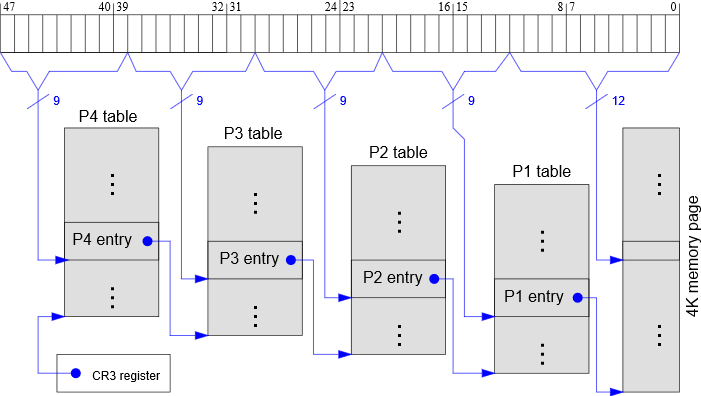
\includegraphics[width=110mm]{images/x86-64-paging.png}
\end{center}
\caption{Paging op de Intel x86-64-processor.}
\label{paging-x86-64}
\end{figure}

Het converteren van een \emph{logisch adres} (d.i. een adres zoals een programma het gebruikt) naar een fysiek adres is zeker niet triviaal. Wanneer de processor voor de instructie \texttt{mov al, [229504h]} het fysieke adres moet berekenen dat overeenkomt met het gevraagde logische adres 229504h, dan moet hij de volgende stappen ondernemen:

\begin{enumerate}
\item{\textbf{Offsets berekenen}} De bits van het hexadecimale adres worden opgesplitst in de verschillende offsets. Voor het adres 229504h geeft dit de volgende resultaten (in decimaal):
    \begin{enumerate}
    \item{Offset in pagina:}\label{PO} 1284
    \item{Page table index:}\label{PTE} 41
    \item{Page directory index:}\label{PDE} 1
    \item{Page directory pointer index:}\label{PDPE} 0
    \item{Page map level 4 index:}\label{PML4} 0
    \end{enumerate}
\item{\textbf{Page map entry zoeken}} De processor gebruikt het adres in register \texttt{CR3} om in het werkgeheugen de page map level 4-tabel te lokaliseren. In deze tabel gebruikt hij de index die hij in stap~\ref{PML4} berekend heeft om de jusite page map level 4 entry (PML4E) op te zoeken. De gevonden entry bevat dan het adres van de page directory pointer tabel die gebruikt moet worden.
\item{\textbf{Page directory pointer entry zoeken}} In de page directory pointer-tabel wordt dan de entry gezocht die overeenkomt met de index die werd berekend in stap~\ref{PDPE}. Deze entry bevat het adres van de page directory die gebruikt moet worden.
\item{\textbf{Page directory entry zoeken}} In de page directory-tabel wordt de entry gezocht die overeenkomt met de index uit stap~\ref{PDE}. In deze entry vinden we het adres van de page table.
\item{\textbf{Page table entry zoeken}} In de page table zoeken we de entry die de informatie bevat over de pagina met het volgnummer uit stap~\ref{PTE}. Deze entry bevat dan het adres van het frame in het werkgeheugen waar de pagina zich bevindt.
\item{\textbf{De gevraagde byte ophalen}} Nu we weten waar de pagina zich in het geheugen bevindt, kunnen we hier de berekende offset (stap~\ref{PO}) bij optellen om uiteindelijk het adres te krijgen van de gevraagde byte.
\end{enumerate}

De bovenstaande berekening moet gebeuren voor \'elke instructie die een adres gebruikt. Het spreekt voor zich dat deze berekening z\'e\'er snel moet uitgevoerd kunnen worden. Alhoewel de page map, page directory pointer, page directory en page table allen in het (trage) werkgeheugen staan, is dit gelukkig geen groot probleem: omdat ze zo vaak opgevraagd worden blijven ze in de processor cache staan. Hierdoor kunnen de tabellen zeer snel uitgelezen worden. Om het een en ander nog te versnellen, voorziet de processor typisch ook een \emph{translation lookaside buffer (TLB)}. Deze component werkt op een gelijkaardige manier als de cache, maar dient expliciet om de resultaten die berekend werden a.d.h.v. de bovenstaande stappen op te slaan voor later hergebruik.

\section{Segmentatie \'en paginatie}

Paginatie laat complexere geheugenbeheerscenario's toe, dus je zou kunnen zeggen dat paginatie beter is dan segmentatie. Uit compatibiliteitsoverwegingen wordt op de Intel x86-architectuur echter zowel segmentatie als paginatie ondersteund\footnote{De Intel x86-64 architectuur die momenteel de standaard is voor desktops en laptops ondersteunt g\'e\'en segmentatie meer, maar enkel paginatie (zoals beschreven in sectie~\ref{multi-level-page-table}).}. Schema~\ref{segmentation_paging} illustreert hoe dit werkt.

\begin{figure}
\begin{center}
\includegraphics[width=110mm]{images/segmentation_paging.png}
\end{center}
\caption{Segmentation en paging support op de Intel x86-processor.}
\label{segmentation_paging}
\end{figure}

Stel dat het actieve programma de instructie \texttt{mov al, [ds:0982CA0Fh]} wil uitvoeren en dat het datasegment (= segment \texttt{ds}) begint op adres 10000000h). Uit Figuur~\ref{segmentation_paging} kunnen we afleiden dat de processor voor de adresberekening de volgende stappen moet volgen:

\begin{enumerate}
\item{\textbf{Descriptor ophalen}} De instructie specifieert dat segment \texttt{ds} gebruikt wordt. De segmentselector wordt uit segmentregister \texttt{ds} gehaald en de overeenkomstige descriptor wordt opgezocht in de globale descriptorentabel. Deze descriptor bevat het basisadres van het segment (10000000h).
\item{\textbf{Logisch adres berekenen}} Het logische adres wordt berekend door bij het basisadres van het segment de verplaatsing (die in de instructie staat) op te tellen. Het resultaat is het logische adres 1982CA0Fh
\item{\textbf{Offsets berekenen}} De bits van het logische adres worden opgesplitst in de verschillende offsets. Voor het adres 1982CA0Fh geeft dit de volgende resultaten (in decimaal):
    \begin{enumerate}
    \item{Offset in pagina:}\label{PO86} 2575
    \item{Page table index:}\label{PTE86} 44
    \item{Page directory index:}\label{PDE86} 102
    \end{enumerate}
\item{\textbf{Page directory entry zoeken}} In de page directory-tabel wordt de entry gezocht die overeenkomt met de index uit stap~\ref{PDE86}. In deze entry vinden we het adres van de page table.
\item{\textbf{Page table entry zoeken}} In de page table zoeken we de entry die de informatie bevat over de pagina met het volgnummer uit stap~\ref{PTE86}. Deze entry bevat dan het adres van het frame in het werkgeheugen waar de pagina zich bevindt.
\item{\textbf{De gevraagde byte ophalen}} Nu we weten waar de pagina zich in het geheugen bevindt, kunnen we hier de berekende offset (stap~\ref{PO86}) bij optellen om uiteindelijk het adres te krijgen van de gevraagde byte.
\end{enumerate}

\section{Virtueel geheugen}

De technieken die in de vorige secties beschreven werden, kunnen gebruikt worden om aan complex geheugenbeheer te doen. Zo kunnen besturingssystemen bijvoorbeeld het concept van \emph{virtueel geheugen} (of \emph{virtual memory}) aanbieden. Hierbij zorgt het besturingssysteem dat het voor elke applicatie \emph{lijkt} alsof ze de hele geheugenruimte ter beschikking hebben. Zo wordt bijvoorbeeld de code van elk proces op de lage adressen geplaatst en de stapel op de hoge adressen. Achter de schermen zorgt het besturingssysteem er d.m.v. paginatie voor dat al deze \emph{virtuele adressen} gemapped worden op andere fysieke adressen, maar vanuit het standpunt van de applicatie ziet zijn geheugenruimte er steeds hetzelfde uit.

Het concept van virtueel geheugen kan ge\"implementeerd worden met behulp van paging \emph{of} segmentatie. In de rest van deze tekst gaan we er van uit dat paging gebruikt wordt, aangezien dit het meest gebruikt wordt in de praktijk en ook geavanceerdere scenario's toelaat.

\subsection{Demand Paging}

In Hoofdstuk~\ref{procesbeheer} werd gezegd dat elk programma dat uitgevoerd wordt in het geheugen moet staan. Het is natuurlijk waar dat een processor enkel instructies kan uitvoeren die in het geheugen staan, maar in de praktijk is het zelden het geval dat elke instructie van een applicatie effectief uitgevoerd wordt (en dus in het geheugen moet staan). Vaak zit er in een programma ook heel wat code voor functionaliteit die amper gebruikt wordt. We kunnen het inladen van het programma dus versnellen door enkel de code in het geheugen te laden die daadwerkelijk gebruikt wordt.

Een techniek die hiervoor gebruikt kan worden is \emph{demand paging}. Een programma wordt in pagina's verdeeld, en enkel de pagina's waar vraag achter is worden in het geheugen geladen. Zo worden enkel pagina's in het geheugen geladen die gebruikt worden; niet-gebruikte pagina's zullen nooit ingeladen worden. Dit heeft een positieve impact op het aantal I/O-operaties dat het besturingssysteem moet doen om het programma in te laden waardoor er minder geheugen nodig is en de computer sneller reageert.

Demand paging vereist wel een aantal hardware-aanpassingen om alles effici\"ent te laten verlopen. De page table entries moeten aangepast worden zodat ze een bit bevatten die aangeeft of de pagina in het geheugen geladen is of niet. Indien dit wel het geval is, dan kan de processor uit de page table entry het adres van het frame ophalen waar de pagina staat. Als de pagina echter niet ingeladen is, dan zal de processor een zogenaamde \emph{page fault} genereren. Dit is een interne interrupt die door het besturingssysteem zal opgevangen worden. Het actieve programma dat de niet-ingeladen pagina opvroeg wordt onderbroken, de interrupt handler laadt de gevraagde pagina in het geheugen, en het programma wordt hervat. Schematisch geeft dat dan Figuur~\ref{demand_paging}.

\begin{figure}
\begin{center}
\includegraphics[width=100mm]{images/demand_paging.png}
\end{center}
\caption{Het demand paging-mechanisme.}
\label{demand_paging}
\end{figure}

\subsection{Swapping}

Zolang er frames in het geheugen vrij zijn, kunnen er nieuwe pagina's ingeladen worden door het demand paging-systeem. Er rijst dan echter de vraag wat er gebeurt indien er zich een page fault voordoet, en het geheugen helemaal vol zit. Het besturingssysteem zal dan niet zomaar een nieuwe pagina kunnen inladen. Omwille van de flexibiliteit van paging hoeft dit echter geen probleem te zijn: het besturingssysteem kan simpelweg een ingeladen pagina (eventueel van een ander proces) uit het geheugen verwijderen, waardoor er plaats vrijkomt. Deze techniek noemt men \emph{swapping}.

De verwijderde pagina mag natuurlijk niet zomaar weggegooid worden. Het programma waartoe de pagina hoort kan ze mogelijk later nog nodig hebben. Daarom worden de verwijderde pagina's opgeslagen op een speciale plaats op de harde schijf: de \emph{swap file} (of soms een \emph{swap partitie}). Toegang tot de swap file is natuurlijk veel trager dan het werkgeheugen, dus het besturingssysteem zal proberen om zo weinig mogelijk te swappen.

De manier waarop het besturingssysteem kiest welke pagina verwijderd moet worden, is belangrijk. Zo mag de pagina best niet in de nabije toekomst terug gebruikt worden. Het besturingssysteem kan dat natuurlijk nooit met zekerheid weten, maar kan wel gokken hoe `populair' een pagina is. Een pagina van een hoge-prioriteitsproces is bijvoorbeeld al een minder goede kandidaat om uit te swappen dan een pagina van een lage-prioriteitsproces.

Swapping laat toe om meer geheugen te gebruiken dan dat er fysisch in de computer zit. Indien de computer 2GB werkgeheugen heeft en een swap file van 1GB, dan kan het besturingssysteem voor 3GB aan data in het geheugen steken. Op eender welk moment zal er natuurlijk maximaal 2GB echt in het fysieke werkgeheugen aanwezig zijn; de rest zit dan in de swap file.

\subsection{Sharing}

Een interessante manier om geheugen uit te sparen is door pagina's tussen processen te delen. Van een programma dat twee keer opgestart wordt, moet er slechts \'e\'en keer het codesegment in het geheugen geplaatst worden. Verschillende programma's gebruiken vaak ook dezelfde bibliotheken die kunnen gedeeld worden. De meeste besturingssystemen reserveren ook een stuk van de virtuele geheugenruimte om pagina's te mappen die de code van de systeemroutines bevatten. Elk proces moet (dezelfde) systeemroutines kunnen oproepen, dus is het logisch dat de code van deze routines gedeeld wordt.

Conceptueel is het delen van pagina's eenvoudig: het besturingssysteem moet in de verschillende page tables van de processen gewoon hetzelfde frame mappen. Beide processen kunnen dan aan de data van dat frame aan. Deze techniek kan perfect gebruikt worden voor effici\"ente inter-proces communicatie. Het ene proces kan bijvoorbeeld data schrijven naar dat frame, wat het andere proces dan kan uitlezen.

Deze eenvoudige manier van delen is echter minder geschikt voor het delen van code. Het is natuurlijk niet wenselijk dat kwaadaardige software de pagina van een gedeelde bibliotheek kan aanpassen die ook door andere programma's gebruikt wordt. Een aanvaller zou zo een bepaalde functie in een bibliotheek kunnen aanpassen om zo de controle van andere programma's over te nemen. Om dit probleem op te lossen, heeft elke pagina \emph{toegangsrechten}. Hiermee kan het besturingssysteem pagina's als \emph{alleen-lezen} (\emph{read only}) markeren, of \emph{niet-uitvoerbaar} (\emph{no-execute}). Pagina's van gedeelde bibliotheken zijn alleen-lezen, waardoor iedereen ze kan lezen en uitvoeren, maar niet aanpassen. Pagina's van de stapel, bijvoorbeeld, zijn meestal niet-uitvoerbaar; de stapel bevat dan ook geen programmacode.

\subsection{Thrasing}

Wanneer veel pagina's van een proces niet in het werkgeheugen geladen zijn, zal het proces vaak onderbroken moeten worden om te swappen. Wanneer het werkgeheugen echter klein is, kan het voorvallen dat de pagina's die uitgeswapt worden snel terug gebruikt worden. In dit geval gaat er veel tijd verloren aan het in- en uitswappen van pagina's. De processor wordt hierdoor te weinig gebruikt (omdat alle processen aan het wachten zijn op pagina's). Wanneer een proces veel tijd verliest aan het in- en uitladen van pagina's, zegt men dat het aan het \emph{trashen} is. Meestal is dit ook niet gelimiteerd tot \'e\'en proces, maar wordt het ganse systeem be\"invloed. Een effectieve (maar drastische) manier om thrashing op te lossen wanneer het zich voordoet, is door programma's af te sluiten en zo geheugen vrij te maken.







\appendix
\chapter{MS-DOS Virussen}

Een belangrijke functie van het besturingssysteem is het beveiligen van het systeem. Met de geconnecteerde wereld die we vandaag kennen, is dit misschien zelfs \'e\'en van de hoofdtaken geworden van het besturingssysteem. Dat is echter niet altijd zo geweest: zoals besproken in Hoofdstuk~\ref{hfdstk:inleiding} is een besturingssysteem origineel ontstaan als een programma om het beheer van processen te vereenvoudigen. Ook het eerste besturingssysteem van Microsoft, het \emph{Microsoft Disk Operating System (MS-DOS)}\index{besturingssysteem!MS-DOS} diende vooral om het procesbeheer te vergemakkelijken en het aansturen van bepaalde hardware (zoals bijvoorbeeld de harde schijf) te vereenvoudigen. Het bood echter geen bescherming. Zo draaide elk proces bijvoorbeeld in kernel mode, waardoor het dus toegang had tot de volledige instructieset die de processor aanbood. Hierdoor kunnen processen rechtstreeks communiceren met hardware en zijn ze dus niet verplicht om via de MS-DOS-aangeleverde routines de hardware te benaderen.

Over het algemeen werkte dit principe goed. Er kon slechts \'e\'en proces tegelijkertijd actief zijn (MS-DOS ondersteunde dus geen multi-programmering), dus kan het actieve proces ook nooit in het vaarwater komen van andere processen aangezien die er niet zijn. De meeste programma's maakten ook gebruik van de services die MS-DOS aanbood om bijvoorbeeld bestanden te openen of uitvoer op het scherm te tonen.

Omdat programma's echter niet gecontroleerd werden door het besturingssysteem, is het niet te verwonderen dat er ook heel wat \emph{malware}\index{malware} gebouwd is geweest voor MS-DOS. Dat nam typische de vorm aan van een virus dat het systeem infecteerde en op bepaalde tijdstippen de correcte werking van het systeem verstoorde. In dit hoofdstuk bespreken we enkele voorbeelden, en leggen we uit waarom deze virussen niet meer kunnen werken in hedendaagse besturingssystemen.

\section{Virussen}

De term \emph{virus}\index{malware!virus}\index{virus} wordt door leken vaak gebruikt voor eender welk stuk software dat een ongewenste en/of kwaadaardige nevenwerking heeft op een computer. Dat is natuurlijk niet correct: een betere term hiervoor is \emph{malware} (wat komt van \emph{malicious software}, of kwaadaardige software). Een virus is een heel specifieke categorie van malware die vroeger veel voorkwam, maar vandaag de dag minder relevant is. De definitie van een virus die wij gebruiken, luidt als volgt:

\begin{quotation}
Een computervirus is een type van kwaadaardige software dat, wanneer het uitgevoerd wordt, zichzelf vermenigvuldigt door aan andere (onschuldige) computerprogramma's een kopie van zichzelf toe te voegen.
\end{quotation}

Cruciaal aan deze definitie is dat een virus dus een bestaand programma aanpast; het bestaat niet op zichzelf. Dit gedrag was belangrijk, want de manier waarop virussen zich vroeger verspreidden was door onschuldige software te infecteren die dan via diskette's onderling tussen mensen werd uitgewisseld. In die tijd wisten computergebruikers precies welk programmabestand overeenkwam met bijvoorbeeld de tekstverwerker die ze gebruikten. Onbekende programma's vielen dus direct op, en zouden niet snel opgestart worden.

Vandaag de dag zijn er veel makkelijkere manieren om malware op een computer te krijgen. De eenvoudige aanpak van de \emph{Happy '99}-worm\index{malware!worm} illustreert dit punt. Rond nieuwjaar 1999 kregen heel wat mensen een email met als onderwerp `Happy 99' die verder leeg was op een bijlage na. Deze bijlage was een uitvoerbaar bestand `Happy99.exe'. Wanneer dit bestand opgestart werd, kreeg de gebruiker vuurwerk te zien (zie Figuur~\ref{happy99}), maar in de achtergrond werd ook het adressenboek doorgenomen en werd de worm doorgestuurd naar elk emailadres dat daarin gevonden werd. Het internet zorgt er voor dat malware zich in een recordtempo op een ongeziene schaal kan verspreiden. Ook gebruiken meer mensen nu een computer, wat er toe leidt dat niet iedereen even goed weet hoe een computer werkt en ook niet iedereen even strikt is in het installeren van belangrijke programma-updates.

\begin{figure}
\begin{center}
\includegraphics[width=70mm]{images/happy99.png}
\end{center}
\caption{De Happy 99-worm}
\label{happy99}
\end{figure}

Virussen voor MS-DOS waren meestal relatief goedaardig. Ze waren veelal een manier om op te scheppen over de technische kwaliteiten die de auteur van zo'n virus had. Zo toonde ze vaak gewoon een bericht op het scherm, eventueel aangevuld met een (tekstuele) tekening. Soms plaagden ze de gebruiker, bijvoorbeeld door de letters van het scherm te laten vallen of door ze te verplichten om eerst een spelletje te spelen. Er waren echter ook kwaadaardige virussen in omloop. Het Casino-virus, bijvoorbeeld, verwijderde de FAT-tabel van de harde schijf en forceerde de gebruiker om een jackpot-spel te spelen. Indien de gebruiker won (waar 17.2\% kans voor was), dan werd een geheugenkopie van de FAT terug naar de schijf gekopie\"eerd. Indien de gebruiker niet won, was hij natuurlijk al zijn bestanden kwijt. Een nog erger voorbeeld was het \emph{CMOSdead}-virus. Dit virus maakte de ROM-chip stuk waar de opstartcode van de computer in stond. Hierdoor kon de computer dus niet meer opstarten. Verder begon hij een irritant lawaai te maken, en formateerde hij de harde schijf indien de gebruiker op CTRL-ALT-DEL drukte.

Onafhankelijk van de goed- of kwaadaardigheid van een virus, staat het vast dat de auteurs bijzonder diepgaande kennis moesten hebben van MS-DOS en computers in het algemeen om zulke software te schrijven. In het bijzonder zijn dit een aantal onderwerpen die je als virusschrijver helemaal onder de knie moest hebben:

\begin{itemize}
\item{\textbf{x86 Assembly}} Virussen moesten klein zijn en gebruikten vaak processorinstructies die niet rechtstreeks bruikbaar zijn vanuit hogere programmeertalen. Daarom werden de meeste virussen ook rechtstreeks in x86 assembly geschreven.
\item{\textbf{Bootproces}} Een populaire plaats om te infecteren was de code van het bootproces. Dit houdt natuurlijk in dat je perfect moet weten wat er allemaal gebeurt wanneer je computer opstart.
\item{\textbf{Interrupts}} De meeste virussen infecteerden de interrupttabel, zodat ze automatisch opgeroepen werden wanneer bepaalde interrupt requests zich voordeden.
\item{\textbf{.EXE-formaat}} Virussen voegden zichzelf toe aan andere programma's. Kennis van het formaat van een .EXE-bestand is dus vereist.
\item{\textbf{Cryptografie/steganografie}} Voor extra bescherming tegen virusscanners kon een virus zichzelf gaan encrypteren of verstoppen.
\end{itemize}

\section{Bootsector-virussen}

Het \emph{Stoned}-virus\footnote{\url{https://en.wikipedia.org/wiki/Stoned_(computer_virus)}} was een voorbeeld van een \emph{bootsector-virus}\index{bootsector-virus}. Deze virussen spitsen zich toe op het infecteren van de opstartcode die op de harde schijf of op een diskette staat. Het Stoned-virus toont in 12.5\% van de keren dat je je computer opstart de zin ``Your PC is now Stoned!'' of ``Legalise Marijuana''. Figuur~\ref{stoned} toont de bootsector van een harde schijf die ge\"infecteerd is met het Stoned-virus. In de rechterkolom kan je onderaan de tekst zien staan.

\begin{figure}
\begin{center}
\includegraphics[width=120mm]{images/stoned.png}
\end{center}
\caption{De bootsector van een ge\"infecteerde computer.}
\label{stoned}
\end{figure}

In Hoofdstuk~\ref{bootproces} hebben we gezien dat moderne computers opstarten volgens de stappen die in de UEFI-standaard vastgelegd zijn. DOS is echter gemaakt voor computers die de voorloper van UEFI gebruikten: het \emph{Basic Input/Output System (BIOS)}. De BIOS is in feite een mini-programma dat de computer initialiseert en op zoek gaat naar een opstartmedium. Als er moet opgestart worden van de harde schijf, dan gaat de BIOS de eerste sector van die schijf (de \emph{Master Boot Record}) in het geheugen laden. De BIOS springt dan naar een miniprogramma dat in de MBR staat (de \emph{Initial Program Loader}, of \emph{IPL}). De IPL zoekt dan tussen de partities van de schijf naar de actieve partitie (d.i. de partitie waar het op te starten besturingssysteem op staat). Wanneer die partitie gevonden is, wordt de eerste sector van die partitie (de \emph{boot sector}) in het geheugen gezet, en springt de IPL naar een mini-programma dat in deze boot sector staat (de \emph{boot loader}). De boot loader is besturingssysteem-afhankelijk en heeft de taak om het besturingssysteem verder op te starten. Figuur~\ref{boot-sequence} toont dit proces schematisch.

\begin{figure}
\begin{center}
\includegraphics[width=125mm]{images/MBR-Boot-Sequence.png}
\end{center}
\caption{Het opstartproces van een computer met BIOS firmware.}
\label{boot-sequence}
\end{figure}

Stel dat de computer een diskette bevat die ge\"infecteerd is met het Stoned-virus. De BIOS controleert tijdens het opstarten of er een diskette in de computer steekt, en als dat het geval is (en als de diskette \emph{bootable} is) gaat hij daarvan opstarten. Dit wil zeggen dat de eerste sector van de diskette naar het geheugen wordt gekopi\"eerd en dat de BIOS springt naar het programma dat hierin vervat zit. Aangezien het om een ge\"infecteerde diskette gaat, is dit programma dus het Stoned-virus dat uitgevoerd wordt. Het eerste wat Stoned doet, is de harde schijf infecteren. De originele master boot record wordt ergens anders op de schijf opgeslagen, en het virus wordt gekopie\"erd. Verder wordt ook interrupt 13h onderschept door eenvoudigweg de interrupttabel aan te passen zodat die naar een methode van het virus wijst. Interrupt 13h wordt door DOS gebruikt voor lees- of schrijfoperaties van sectoren. Het resultaat is dat elke lees- of schrijfoperatie die uitgevoerd wordt door eender welk programma het virus activeert. Wanneer het virus een onge\"infecteerde diskette detecteert, dan infecteert hij die eerst alvorens de originele interrupt-aanvraag te verwerken.

\section{Executable infectors}

Het \emph{Phantom1}-virus is een voorbeeld van een \emph{executable infector}\index{executable infector}. Deze virussen plaatsen een kopie van zichzelf in de programma's die de gebruiker uitvoert. Phantom1 wordt geactiveerd wanneer er ongeveer 20 minuten geen toetsenbordactiviteit is. Het toetsenbord wordt gedeactiveerd en de gebruiker krijgt een boodschap te zien en een geanimeerd doodshoofd (zie Figuur~\ref{phantom1}).

\begin{figure}
\begin{center}
\includegraphics[width=80mm]{images/Phantom1.png}
\end{center}
\caption{Het Phantom1-virus in actie.}
\label{phantom1}
\end{figure}

Het virus kent de structuur van een uitvoerbaar bestand, en weet dat in de hoofding van een .EXE-bestand het adres staat van de instructie waarmee het programma op moet starten. Het virus kan zichzelf dus toevoegen aan het code sectie en kan dit opstartadres in de hoofding overschrijven. Wanneer het programma dan opgestart wordt, zal het eerst de code van het virus opstarten alvorens het virus terugspringt naar de normale opstartprocedure van het programma.

Phantom1 past ook de interrupttabel aan, meerbepaald de adressen voor de interrupts 1Ch en 21h. Interrupt 1Ch wordt periodiek opgeroepen door de klok van het systeem, terwijl interrupt 21h door DOS gebruikt wordt voor onder andere allerlei bestandsoperaties en het inlezen van toetsenbordinvoer. Hierdoor kan Phantom1 meten wanneer er 20 minuten geen toetsenbordactiviteit is geweest. Ook wanneer er een nieuw programma opgestart wordt, zal DOS interrupt 21h activeren. Phantom1 gaat in dit geval het programma meteen infecteren.

\section{De viruswapenwedloop}

Naarmate MS-DOS meer last begon te krijgen van virussen, werd er gezocht naar oplossingen om deze virussen te kunnen detecteren of zelfs verwijderen. Al snel na de eerste virussen kwam ook de eerste generatie van virusscanners\index{virusscanner}. Om slechts een kleine impact op de snelheid van het systeem te hebben, werkten deze scanners nogal eenvoudig. Zo werd de harde schijf bijvoorbeeld een eerste keer gescanned en werd er een database bijgehouden van alle groottes van de uitvoerbare bestanden. Periodiek werd de harde schijf dan terug gescanned en werd de grootte van alle programma's vergeleken met de data van de database. Als er een programma \emph{gegroeid} was, dan was het waarschijnlijk ge\"infecteerd door een virus. Deze aanpak was natuulijk eenvoudig te omzeilen: in plaats van de code van het virus achter het originele programma te plakken, werd er gewoon een stuk van het originele programma overschreven. Mettertijd werden de virusscanners dan ook geavanceerder en gingen ze meer op zoek gaan naar bepaalde patronen die op een virusinfectie konden wijzen (bijv. een opeenvolging van bepaalde instructies). Naarmate dat virusscanners beter werden, werden ook de virussen beter. Er ontstond dus als het ware een wapenwedloop tussen de auteurs van de virussen en de auteurs van de virusscanners.

Een \emph{stealth virus}\index{virus!stealth} verborg de aanpassingen die het gemaakt had aan het systeem. Dit werd onder andere gedaan door de systeemfunctie om sectoren te lezen te kapen. De resultaten van deze functie werden dan vervalst, zodat het oproepend programma de infectie niet zou kunnen waarnemen.

Een \emph{polymorf virus}\index{virus!polymorf} produceerde werkende kopie\"en van zichzelf die er allen verschillend uitzagen. Op die manier kon een virusscanner niet zoeken naar een bepaald vast patroon dat in het virus voorkwam, aangezien elke kopie van het virus er anders uitzag. Een relatief eenvoudige manier om het gewenste effect te bekomen, was door het virus zichzelf te laten encrypteren.

Een \emph{gepantserd virus}\index{virus!gepantserd} maakte gebruik van allerlei anti-debugging trucs en gebruikte code die expres moeilijk en onlogisch in elkaar zat. Dit maakte het werk van de virusanalisten moeilijker, zodat het langer duurde eer er een virusscanner was die een effectieve beveiliging vormde tegen het virus.

Ondertussen is MS-DOS vervangen door Windows, en geeft het besturingssysteem niet meer de volledige toegang tot de hardware aan eender welke applicatie. Heel wat technologie\"en die we in de vorige hoofdstukken gezien hebben zorgen er voor dat een virus vandaag niet meer zo effectief zou zijn als het ooit was. Zo bevat een modern besturingssysteem bijvoorbeeld deze tegenmaatregelen:

\begin{itemize}
\item{\textbf{UEFI Secure Boot}} Alle code die uitgevoerd wordt tijdens het opstartproces wordt cryptografisch ondertekend. Alvorens de processor de code uitvoert, wordt steeds de handtekening gecontroleerd. Mocht de originele code veranderd zijn, dan zal de handtekening niet meer kloppen en zal de UEFI-implementatie de code niet uitvoeren.
\item{\textbf{Geheugenbescherming}} Programma's worden uitgevoerd in afgeschermde stukken geheugen. Het ene programma kan dus niet zomaar een stuk geheugen aanpassen van een ander programma of van het besturingssysteem.
\item{\textbf{Bestandspermissies}} Besturingssystemen dwingen bestandspermissies af, waardoor een bestand bijvoorbeeld leesbaar kan zijn maar niet schrijfbaar. In Windows zijn bijvoorbeeld de programma's die op de standaardplek ge\"installeerd worden (c:\textbackslash{}Program Files) \emph{niet} schrijfbaar.
\item{\textbf{Codehandtekeningen}} De code in programma's kan een cryptografische handtekening krijgen. Wanneer het besturingssysteem zo'n handtekening controleert en die niet overeenstemt met de feitelijke code, dan zal het programma niet opgestart worden.
\item{\textbf{Monitoring van hardwaretoegang}} Elke toegang tot een hardwareapparaat verloopt via het besturingssysteem. Een programma kan dus niet rechtstreeks communiceren met hardware. Het besturingssysteem krijgt steeds de kans om de toegang te monitoren en eventueel te verbieden.
\item{\textbf{Geavanceerde virusscanners}} Hedendaagse virusscanners doen veel meer dan het zoeken naar bepaalde patronen in code. Wanneer het voor een virusscanner niet duidelijk is of een bepaald stuk van een programma een virus zou kunnen zijn (bijv. omdat het virus zich ge\"encrypteerd heeft), dan kan de virusscanner de verdachte code emuleren. De code wordt dan als het ware uitgevoerd onder veilige omstandigheden en geanalyseerd.
\end{itemize} 

\printindex

\end{document}
